%%%%%%%%%%%%%%%%%%%%%%%%%%%%%%%%%%%%%%%%%%%%%%%%%%%%%%%%%%%%
%  Trinary: A Ternary (Base-3) Computer Simulation
%  Full Technical Monograph — COMPACT EDITION
%%%%%%%%%%%%%%%%%%%%%%%%%%%%%%%%%%%%%%%%%%%%%%%%%%%%%%%%%%%%
\documentclass[10pt,a4paper,twoside]{book}

% -- Packages ----------------------------------------------
\usepackage[utf8]{inputenc}
\usepackage[T1]{fontenc}
\usepackage{amsmath,amssymb,amsthm}
\usepackage{graphicx}
\usepackage{hyperref}
\usepackage{booktabs}
\usepackage{longtable}
\usepackage{array}
\usepackage{multirow}
\usepackage{verbatim}
\usepackage{fancyhdr}
\usepackage{geometry}
\usepackage{setspace}
\usepackage{tocloft}
\usepackage{caption}
\usepackage{subcaption}
\usepackage{listings}
\usepackage{xcolor}
\usepackage{float}
\usepackage{csquotes}
\usepackage{pmboxdraw}
\usepackage{enumitem}

% -- Modern fonts ------------------------------------------
\usepackage{tgheros}            % TeX Gyre Heros (sans-serif, Google Sans-like)
\renewcommand{\familydefault}{\sfdefault}  % Sans-serif as body text

% -- Page geometry -----------------------------------------
\geometry{margin=0.65in}
\singlespacing
\setlength{\parskip}{0pt}
\setlength{\parindent}{1em}

% -- Compact spacing ---------------------------------------
\setlength{\floatsep}{6pt plus 2pt minus 2pt}
\setlength{\textfloatsep}{8pt plus 2pt minus 2pt}
\setlength{\intextsep}{6pt plus 2pt minus 2pt}
\setlength{\dblfloatsep}{6pt plus 2pt minus 2pt}
\setlength{\abovecaptionskip}{4pt}
\setlength{\belowcaptionskip}{4pt}
\setlist{nosep,leftmargin=*}
\setlength{\partopsep}{0pt}
\setlength{\parsep}{0pt}
\setlength{\itemsep}{0pt}
\setlength{\topsep}{0pt}

% -- Compact TOC -------------------------------------------
\setlength{\cftbeforechapskip}{4pt}
\setlength{\cftbeforesecskip}{2pt}
\setlength{\cftbeforesubsecskip}{1pt}



% -- Hyperlinks --------------------------------------------
\hypersetup{
    colorlinks=true,
    linkcolor=blue,
    citecolor=blue,
    urlcolor=blue,
}

% -- Listings style ----------------------------------------
\definecolor{asmcomment}{rgb}{0.25,0.5,0.25}
\definecolor{asmopcode}{rgb}{0.0,0.5,0.7}
\definecolor{asmreg}{rgb}{0.7,0.5,0.0}
\lstdefinelanguage{TernaryAsm}{
    morekeywords={LOAD,MOV,CLR,ADD,SUB,MUL,DIV,AND,OR,NOT,CMP,JMP,JZ,JNZ,PUSH,POP,CALL,RET,HALT,STOREM,LOADM,INT,IRET,EI,DI,SETIVT,SETTIMER,TLOADW,TSTOREW,TVECADD,TMATMUL,TDOT,TACT},
    morecomment=[l]{\#},
    morecomment=[l]{;},
    sensitive=false,
}
\lstset{
    language=TernaryAsm,
    basicstyle=\footnotesize\ttfamily,
    commentstyle=\color{asmcomment},
    keywordstyle=\color{asmopcode}\bfseries,
    stringstyle=\color{asmreg},
    breaklines=true,
    columns=fullflexible,
    frame=single,
    numbers=left,
    numberstyle=\tiny,
    abovecaptionskip=2pt,
    belowcaptionskip=2pt,
}

% -- Theorem environments ----------------------------------
\newtheorem{definition}{Definition}[chapter]
\newtheorem{theorem}{Theorem}[chapter]
\newtheorem{lemma}{Lemma}[chapter]

% Abstract environment (not defined by default in book class)
\newenvironment{abstract}
  {\chapter*{Abstract\markboth{Abstract}{Abstract}}}
  {\vfill\noindent\textit{Keywords:} ternary computing, base-3, computer architecture,
   CPU simulation, neural networks, hardware simulation, web visualizer\newpage}

\begin{document}

% -- Suppress blank pages -----------------------------------
\let\cleardoublepage\clearpage

% +==========================================================+
% |                    FRONT MATTER                         |
% +==========================================================+

\title{Trinary: A Ternary (Base-3) Computer Simulation\\
       \large Complete Architecture, Implementation, and Analysis}
\author{Devak Chaudhari}
\date{\today}

\maketitle

\begin{abstract}
We present Trinary, a complete ternary (base-3) computer system simulated entirely in
software. Spanning from fundamental ternary logic gates through a 27-opcode central
processing unit, two-pass assembler, machine-code encoder, dual memory-mapped display
subsystems, a Fantasy Console software development kit, a structured-language compiler
(TAL), cycle-accurate hardware microarchitecture simulation, a tensor accelerator
coprocessor with GPU-mode parallel computing, ternary neural networks, and a WebSocket-
based web visualizer, Trinary serves as both an educational platform for computer
architecture and a research vehicle for non-binary computing systems. The system comprises
approximately 28,000 lines of Python and C code, validated by a test suite of 594 unit
tests across all subsystems. A native C backend provides up to 13$\times$ speedup on
arithmetic-heavy workloads through an auto-detected ctypes bridge. This monograph presents
the complete architecture, design rationale, implementation details, and performance
characteristics of the Trinary system across 44 chapters with full instruction-set
reference, hardware specifications, benchmark data, and appendix reference.
\end{abstract}

\tableofcontents

\part{Foundations}

%====================================================================
\chapter{Introduction to Ternary Computing}
\label{ch:intro}

\section{Binary and Its Alternatives}

Since the earliest electronic computers, the binary number system (base~2) has dominated
digital computing. This dominance is not due to mathematical optimality but to engineering
pragmatism: two-state electronic circuits (on/off, high/low, charged/discharged) are
reliable, simple to manufacture, and map naturally to Boolean algebra. The vacuum-tube
and later transistor-based logic families that emerged in the mid-20th century were
inherently binary, and the entire semiconductor industry optimized around this
paradigm for decades.

Yet from an information-theoretic standpoint, base~2 is not the most efficient radix.
Consider the problem of representing numbers up to some maximum value $N$ using a fixed
number of digit positions. The number of distinct values representable with $d$ digits in
base~$b$ is $b^d$. For a given $b$, the number of digits required to represent $N$ is
$\lceil\log_b N\rceil$, and the total ``cost'' in terms of digit states is $b \cdot
\lceil\log_b N\rceil$. Minimizing this cost over $b$ yields the optimal radix.

\section{The Optimal Radix Problem}

\begin{definition}[Radix efficiency]
For a base~$b$, the number of distinct states per digit is $b$, and the number of digits
needed to represent a value up to $N$ is approximately $\log_b N$. The product
$C(b) = b \cdot \log_b N$ represents a figure of merit, where lower values indicate
greater efficiency.
\end{definition}

Treating $b$ as a continuous variable and ignoring the ceiling, we have:
\[
C(b) = b \cdot \frac{\ln N}{\ln b} = (\ln N) \cdot \frac{b}{\ln b}.
\]
Minimizing $f(b) = b / \ln b$ with respect to $b$:
\[
f'(b) = \frac{\ln b - 1}{(\ln b)^2} = 0 \implies \ln b = 1 \implies b = e \approx 2.718.
\]
Thus the mathematically optimal radix is $e$, making base~3 (ternary) the most efficient
integer base. This result was noted by Knuth~\cite{knuth1997art} and has been confirmed
by multiple analyses~\cite{hurts1989comparison}.

In practice, ternary offers approximately 37\% fewer digits than binary for representing
equivalent values. For a value of 1,000,000, binary requires 20 digits
(11110100001001000000$_2$) while ternary requires only 13 (1212210202001$_3$). This
translates to potential savings in memory, bus width, and power consumption.

\section{Historical Ternary Computers}

The most significant historical implementation of ternary computing was the Soviet Setun
computer~\cite{brusentsov1965setun}, developed at Moscow State University in 1958 under
the direction of Nikolay Brusentsov. The Setun used \emph{balanced ternary} with digits
$\{-1,0,1\}$, implemented using ferrite-core memory and vacuum-tube logic. Key
specifications included:

\begin{itemize}
    \item Word size: 18 trits (approximately 28.5 bits of information);
    \item Memory: 162 words of ferrite-core storage (expandable to 486);
    \item Performance: approximately 4,500 operations per second;
    \item Number representation: balanced ternary with no separate sign bit;
    \item Total production: approximately 50 units.
\end{itemize}

The Setun demonstrated several advantages over contemporary binary machines: simpler
arithmetic (addition and subtraction are identical operations in balanced ternary),
inherent signed representation, and more efficient number storage. However, the
binary-oriented semiconductor industry and the dominance of the von Neumann architecture
with binary logic gates prevented ternary computing from achieving widespread adoption.

Subsequent research in multiple-valued logic (MVL)~\cite{smith1997mvl} has explored
quaternary (base-4), quinary (base-5), and other radices, but no other ternary computer
has been commercially produced.

\section{Motivation for Trinary}

Modern computing faces several challenges that warrant revisiting alternative number
systems:
\begin{itemize}
    \item Power consumption: ternary arithmetic circuits can, in theory, perform more
          computation per switching event than binary equivalents;
    \item Memory wall: ternary's improved digit density could reduce memory traffic;
    \item Educational value: studying non-binary architectures deepens understanding of
          computer architecture fundamentals;
    \item Research platform: a complete, executable ternary system enables experimentation
          with ternary algorithms, compilers, and operating systems.
\end{itemize}

Trinary addresses these motivations by providing a fully functional ternary computer
simulation with a complete software stack. The system spans 34 chapters of
documentation, approximately 28,000 lines of source code, and 594 automated tests.

\section{Scope of This Monograph}

This work presents the complete Trinary system across 44 chapters organized into eight
parts:
\begin{itemize}
    \item \textbf{Part I -- Foundations}: Chapters~\ref{ch:intro}--\ref{ch:memory}
          cover ternary number representation, logic gates, adder circuits, arithmetic
          via decimal round-trip, the arithmetic logic unit (ALU), register file, and
          memory architecture;
    \item \textbf{Part II -- CPU Architecture}: Chapters~\ref{ch:cpu}--\ref{ch:timer}
          detail the 27-opcode instruction set, fetch-decode-execute cycle, data
          movement and arithmetic instructions, control flow, subroutines, stack
          operations, memory access, interrupts, and timer;
    \item \textbf{Part III -- Toolchain}: Chapters~\ref{ch:assembler}--\ref{ch:tal}
          describe the two-pass assembler, machine-code encoder/decoder, and TAL
          structured-language compiler;
    \item \textbf{Part IV -- Software Environment}: Chapters~\ref{ch:display}--
          \ref{ch:sdk} cover the memory-mapped display, operating system shell, PyQt6
          visual simulator, demo games, dual display system, and Fantasy Console SDK;
    \item \textbf{Part V -- Acceleration}: Chapters~\ref{ch:accelerator}--\ref{ch:native}
          present the tensor accelerator coprocessor, GPU mode, SIMD processing, packed
          trit storage, and native C backend;
    \item \textbf{Part VI -- Hardware Simulation}: Chapter~\ref{ch:hardware} describes
          the cycle-accurate microarchitecture simulation including pipeline, cache,
          branch predictor, bus, DMA, interrupt controller, VRAM controller, profiler,
          and all subcomponents in detail;
    \item \textbf{Part VII -- Artificial Intelligence}: Chapter~\ref{ch:nn} covers
          the ternary neural network framework including TritTensor, perceptron,
          activation functions, loss functions, dual optimiser strategies, and
          supervised training;
    \item \textbf{Part VIII -- Web Visualizer}: Chapter~\ref{ch:webviz} describes
          the browser-accessible FastAPI + React visualizer interface, WebSocket
          protocol, snapshot engine, and seven-panel visualisation workspace.
\end{itemize}

%====================================================================
\chapter{System Architecture Overview}
\label{ch:arch}

\section{Five-Layer Abstraction Stack}

Trinary follows a five-layer abstraction stack, each layer building on the one below:

\begin{enumerate}
    \item \textbf{Logic Layer}: Ternary logic gates (TNOT, TAND, TOR) operating on
          single trits. Implemented in \texttt{logic.py}.
    \item \textbf{ALU Layer}: Arithmetic and logical operations via decimal round-trip
          (for signed arithmetic) or native ripple-carry addition (for educational use).
          Implemented in \texttt{alu.py}, \texttt{arithmetic.py}, and \texttt{adder.py}.
    \item \textbf{CPU Layer}: Fetch-decode-execute cycle with 27 opcodes, 4 general-
          purpose registers, dual stacks (memory-based PUSH/POP and Python-list
          CALL/RET), interrupt system, and timer. Implemented in \texttt{cpu.py}.
    \item \textbf{Assembler Layer}: Two-pass assembly with symbolic labels and
          machine-code encoding. Implemented in \texttt{assembler.py} and

\begin{figure}[H]
\centering
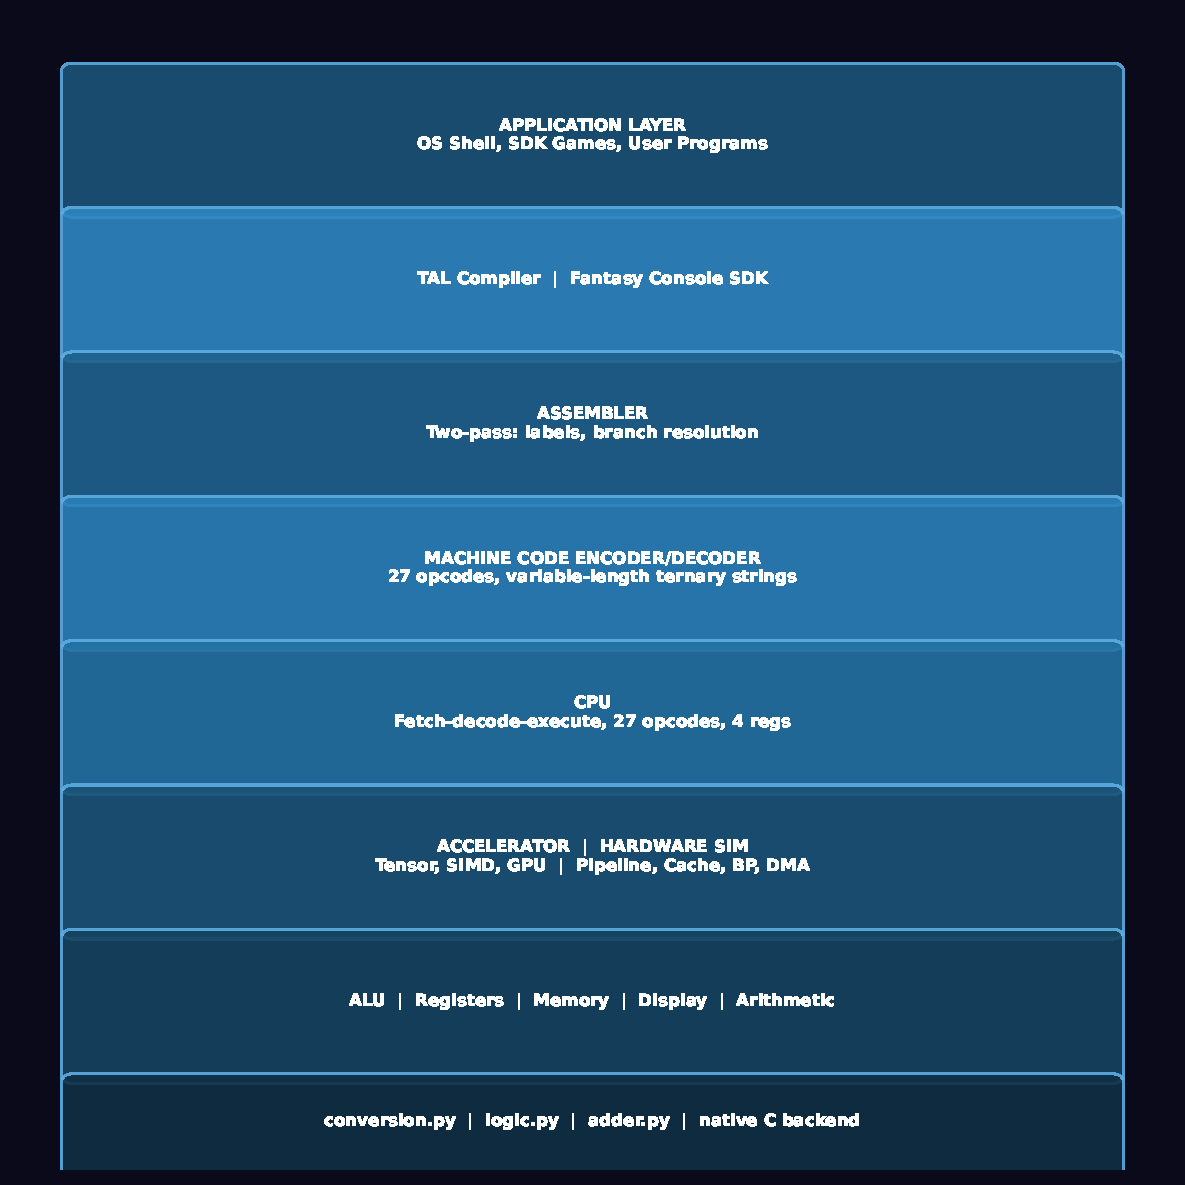
\includegraphics[width=0.72\textwidth]{system_stack.pdf}
\caption{Five-layer abstraction stack — from ternary logic gates through assembler, CPU, ALU, to the OS and display layers}
\label{fig:sysstack}
\end{figure}
          \texttt{machine.py}.
    \item \textbf{OS/Application Layer}: Operating system shell (legacy TTY and modular
          SDK), Fantasy Console SDK, demo games, and user programs. Implemented in
          \texttt{os.py}, \texttt{os/}, \texttt{sdk/}, and \texttt{demo\_games.py}.
\end{enumerate}

\section{Package Structure}

The source package \texttt{src/trinary/} contains the following modules:

\begin{verbatim}
src/trinary/
+-- conversion.py        Base conversion (ternary/decimal/binary)
+-- logic.py             Ternary logic gates
+-- adder.py             Native base-3 ripple-carry adder
+-- arithmetic.py        Decimal round-trip arithmetic
+-- alu.py               Arithmetic logic unit
+-- registers.py         Register file (R0-R3)
+-- memory.py            Addressable RAM
+-- cpu.py               CPU (27 opcodes, dual stacks, interrupts)
+-- assembler.py         Two-pass assembler
+-- machine.py           Machine-code encoder/decoder
+-- tal.py               TAL structured-language compiler
+-- native_backend.py    C ctypes bridge (auto-detect)
+-- os.py                Legacy TTY OS shell
+-- os/                  Modular SDK OS package
+-- display/             Dual display subsystem
+-- sdk/                 Fantasy Console SDK
+-- accelerator/         Tensor accelerator coprocessor
+-- hardware/            Cycle-accurate hardware simulation
+-- ui/                  PyQt6 desktop visual simulator
+-- ai/                  Ternary neural networks
\end{verbatim}

\section{Complete System Stack}

The full system stack, from hardware primitives to application software:

\begin{verbatim}
+--------------------------------------------------------------+
|  APPLICATION LAYER                                           |
|  (OS Shell, Demo Programs, User Code, Fantasy Console Games) |
+------------------------------+-------------------------------|
|  TAL COMPILER                |  FANTASY CONSOLE SDK          |
|  (structured lang→assembly)  |  (Engine, Runtime, Cartridge) |
+------------------------------+-------------------------------|
|  ASSEMBLER                                                   |
|  (two-pass: labels→addresses, branch resolution)              |
+--------------------------------------------------------------|
|  MACHINE CODE ENCODER / DECODER                              |
|  (assembly <-> ternary opcode strings, 27 opcodes)              |
+--------------------------------------------------------------|
|  CPU                                                         |
|  (fetch-decode-execute, 27 opcodes, 4 regs, 512/10000B RAM) |
+----------------------+---------------------------------------|
|  ACCELERATOR COPROC  |  HARDWARE SIMULATION                  |
|  (TensorMemory, SIMD,|  (Pipeline, Cache, Branch Pred,      |
|   TensorCore, GPU)   |   DMA, Bus, Interrupts, VRAM, Prof)  |
+----------------------+---------------------------------------|
|  ALU | REGISTERS | MEMORY | DISPLAY | ARITHMETIC             |
+--------------------------------------------------------------|
|  conversion.py | logic.py | adder.py | native C backend      |
+--------------------------------------------------------------+
\end{verbatim}

\section{Memory Maps}

Trinary supports two memory configurations. The default configuration provides 512
addressable cells, while an extended configuration with 10,000 cells supports the
SDK framebuffer subsystem.

\begin{table}[H]
\centering
\caption{Default memory map (512 addresses)}
\label{tab:memmap_default}
\begin{tabular}{lcl}
\toprule
Address Range & Size & Purpose \\
\midrule
0--127 & 128 & General data / program storage \\
128--199 & 72 & Stack (grows down from 255) \\
200--255 & 56 & Video RAM (7 rows $\times$ 8 cols) \\
256--259 & 4  & Reserved \\
260      & 1  & Keyboard buffer \\
261--511 & 251 & Available \\
\bottomrule
\end{tabular}
\end{table}

\begin{table}[H]
\centering
\caption{Extended memory map (10,000 addresses, SDK mode)}
\label{tab:memmap_extended}
\begin{tabular}{lcl}
\toprule
Address Range & Size & Purpose \\
\midrule
0--999    & 1,000 & General data / program / stack \\
1000--5095 & 4,096 & SDK framebuffer VRAM (64$\times$64 pixels, 9 colors) \\
5096--8999 & 3,904 & Available \\
9000      & 1     & SDK keyboard data register \\
9001      & 1     & SDK keyboard status register \\
9002--9999 & 998   & Available \\
\bottomrule
\end{tabular}
\end{table}

\section{Number Representation}

Trinary uses \emph{signed-magnitude} representation:
\begin{itemize}
    \item Positive numbers: standard ternary strings (each digit $d_i \in \{0,1,2\}$,
          most significant digit first). E.g., \texttt{"10"} = $1\cdot 3^1 + 0\cdot 3^0
          = 3$ decimal.
    \item Negative numbers: leading minus sign followed by the magnitude. E.g.,
          \texttt{"-10"} = $-3$ decimal.
    \item Zero: the string \texttt{"0"}.
\end{itemize}

This is not balanced ternary (which uses digits $\{-1,0,1\}$). The signed-magnitude
convention was chosen for simplicity of implementation and clarity for educational use.
The tradeoff is that arithmetic must handle sign separately from magnitude, which the
decimal round-trip approach naturally accommodates.

%====================================================================
\chapter{Environment Setup and Testing}
\label{ch:setup}

\section{Prerequisites and Installation}

The system requires Python 3.10 or later and a C compiler (gcc or clang) for the native
backend. Installation is via standard Python packaging:

\begin{verbatim}
pip install -e .
\end{verbatim}

The \texttt{-e} (editable) flag ensures that changes to source files in
\texttt{src/trinary/} take effect immediately without re-installation. The package is
registered as \texttt{trinary}.

\section{Running Tests}

The complete test suite is run with pytest:

\begin{verbatim}
python -m pytest tests/ -v          # All 594 tests
python -m pytest tests/test_cpu.py -v     # CPU-specific tests
python -m pytest tests/ -k "cmp" -v       # Keyword filter
\end{verbatim}

The test suite completes in approximately 0.4 seconds on modern hardware, providing
rapid feedback during development.

\section{Running the System}

Several entry points are available:

\begin{verbatim}
python -m trinary.os                 # Boot legacy OS shell (TTY)
python -m trinary.ui.app             # PyQt6 desktop UI (needs PyQt6)
python -m trinary.demo_games pong    # SDK game demo
python -m trinary.native_benchmark   # Python vs C benchmark
python test_snake_tal.py             # TAL-compiled snake (13 frames)
\end{verbatim}

%====================================================================
\chapter{Trit: The Fundamental Unit}
\label{ch:trit}

\section{Definition}

A \emph{trit} (ternary digit) is the base-3 analogue of a binary bit. It is the atomic
unit of information in the Trinary system.

\begin{definition}
A trit $t$ is an element of the set $\{0,1,2\}$, representing the three possible states
of a ternary digit.
\end{definition}

The ternary representation of a non-negative integer $n$ is a string
$t_{k-1}t_{k-2}\ldots t_0$ such that
\[
n = \sum_{i=0}^{k-1} t_i \cdot 3^i,\quad t_i \in \{0,1,2\},
\]
where $k$ is the number of trits required. The most significant trit $t_{k-1}$ is
non-zero by convention (except for the value zero itself, represented as \texttt{"0"}).

\section{Digit Efficiency}

Ternary is more digit-efficient than binary: for a value $N$, the number of digits
required in base $b$ is $\lceil \log_b N \rceil$. The ratio of binary to ternary digits
is approximately $\log_2 3 \approx 1.585$, meaning ternary requires about 37\% fewer
digits than binary for equivalent values.

\begin{table}[H]
\centering
\caption{Digit comparison: binary vs.\ ternary}
\label{tab:digits}
\begin{tabular}{crrr}
\toprule
Value & Binary Digits & Ternary Digits & Savings \\
\midrule
10     & 4  & 3  & 25\% \\
100    & 7  & 5  & 29\% \\
1,000  & 10 & 7  & 30\% \\
10,000 & 14 & 9  & 36\% \\
100,000 & 17 & 11 & 35\% \\
1,000,000 & 20 & 13 & 35\% \\
\bottomrule
\end{tabular}
\end{table}

This efficiency has practical implications for memory density and bus width in ternary
hardware designs.

%====================================================================
\chapter{Base Conversion Systems}
\label{ch:conversion}

Trinary implements a complete suite of conversion functions in \texttt{conversion.py}.
All functions handle signed-magnitude negative numbers, zero, invalid input detection,
and edge cases. The conversion layer is the bridge between the user's mental model
(decimal integers) and the CPU's internal representation (ternary strings), and is
used by every other subsystem — the assembler (for immediate values), the ALU (for
decimal round-trip arithmetic), the display (for ASCII codes), and the neural network
framework (for signed-offset encoding).

\section{Conversion Algorithms}

\begin{description}
    \item[\texttt{ternary\_to\_decimal(s)}]: Processes the string right-to-left,
          accumulating $d_i \cdot 3^i$ for each position. For negative strings (leading
          \texttt{-}), the sign is applied after conversion.
          \newline Example: \texttt{"1021"} $\rightarrow 1\cdot3^3 + 0\cdot3^2 + 2\cdot3^1 + 1\cdot3^0 = 27 + 0 + 6 + 1 = 34$.
    \item[\texttt{decimal\_to\_ternary(n)}]: Repeatedly divides by 3, collecting
          remainders. For negative $n$, the sign is prepended after conversion.
          \newline Example: $34 \rightarrow 34 \div 3 = 11\ \text{r}\ 1,\ 11 \div 3 = 3\ \text{r}\ 2,\ 3 \div 3 = 1\ \text{r}\ 0,\ 1 \div 3 = 0\ \text{r}\ 1 \rightarrow \texttt{"1021"}$.
    \item[\texttt{ternary\_to\_binary(s)}]: Converts ternary to decimal, then decimal
          to binary. Useful for interop with standard computing tools.
    \item[\texttt{binary\_to\_ternary(s)}]: Converts binary to decimal, then decimal
          to ternary.
\end{description}

\section{Edge Case Handling}

The conversion functions handle the following edge cases explicitly:
\begin{itemize}
    \item \textbf{Zero}: \texttt{"0"} converts to 0 and back, regardless of sign.
    \item \textbf{Leading zeros}: \texttt{"0012"} is treated as \texttt{"12"} (decimal 5)
          since the leading zeros do not affect the numeric value.
    \item \textbf{Empty strings}: Raise \texttt{ValueError}.
    \item \textbf{Very large values}: No hard-coded upper bound; performance degrades
          linearly with string length.
    \item \textbf{Negative zero}: \texttt{"-0"} is accepted but treated as 0.
\end{itemize}

\section{Validation}

Companion functions validate input strings:
\begin{description}
    \item[\texttt{validate\_ternary(s)}]: Checks that all characters are \texttt{0},
          \texttt{1}, or \texttt{2}, with optional leading \texttt{-}.
    \item[\texttt{validate\_binary(s)}]: Checks that all characters are \texttt{0}
          or \texttt{1}.
\end{description}

Invalid inputs raise descriptive errors, ensuring that all downstream operations
receive well-formed data. The validation functions are used as the first line of
defense in the ALU, assembler, and machine-code encoder.

%====================================================================
\chapter{Ternary Logic Gates}
\label{ch:gates}

Ternary logic extends Boolean algebra to three truth values. We define three primitive
gates following the conventions of Kleene's strong three-valued logic and prior work in
multiple-valued logic~\cite{smith1997mvl,epstein1985mvl}.

\section{Definitions}

\begin{definition}[TNOT]
\[
\texttt{tnot}(x) = 2 - x
\]
This maps 0$\rightarrow$2, 1$\rightarrow$1, 2$\rightarrow$0.
\end{definition}

\begin{definition}[TAND]
\[
\texttt{tand}(x, y) = \min(x, y)
\]
Element-wise minimum of the two trits.
\end{definition}

\begin{definition}[TOR]
\[
\texttt{tor}(x, y) = \max(x, y)
\]
Element-wise maximum of the two trits.
\end{definition}

These definitions correspond to the interpretation where 0 = false, 1 = unknown/neutral,
and 2 = true. In this system:
\begin{itemize}
    \item TNOT generalizes logical negation: false becomes true, true becomes false, and
          the neutral value remains unchanged.
    \item TAND generalizes logical conjunction: the result is true only when both
          operands are true; if either is false, the result is false.
    \item TOR generalizes logical disjunction: the result is true if either operand
          is true; if both are false, the result is false.
\end{itemize}

\section{Truth Tables}

\begin{table}[H]
\centering
\caption{TNOT truth table}
\label{tab:tnot}
\begin{tabular}{c|c}
$x$ & $\texttt{tnot}(x)$ \\ \midrule
0 & 2 \\
1 & 1 \\
2 & 0
\end{tabular}
\qquad
\begin{tabular}{cc|c}
$x$ & $y$ & $\min(x,y)$ \\ \midrule
0 & 0 & 0 \\
0 & 1 & 0 \\
0 & 2 & 0 \\
1 & 1 & 1 \\
1 & 2 & 1 \\
2 & 2 & 2
\end{tabular}
\qquad
\begin{tabular}{cc|c}
$x$ & $y$ & $\max(x,y)$ \\ \midrule
0 & 0 & 0 \\
0 & 1 & 1 \\
0 & 2 & 2 \\
1 & 1 & 1 \\
1 & 2 & 2 \\
2 & 2 & 2
\end{tabular}
\end{table}

\section{Algebraic Properties}

The ternary logic gates satisfy the following algebraic laws:
\begin{itemize}
    \item Idempotence: $\texttt{tand}(x, x) = x$ and $\texttt{tor}(x, x) = x$
    \item Commutativity: $\texttt{tand}(x, y) = \texttt{tand}(y, x)$ and
          $\texttt{tor}(x, y) = \texttt{tor}(y, x)$
    \item Associativity: both operations are associative
    \item Distributivity: $\texttt{tand}(x, \texttt{tor}(y, z)) =
          \texttt{tor}(\texttt{tand}(x, y), \texttt{tand}(x, z))$
    \item De Morgan's laws: $\texttt{tnot}(\texttt{tand}(x, y)) =
          \texttt{tor}(\texttt{tnot}(x), \texttt{tnot}(y))$ and
          $\texttt{tnot}(\texttt{tor}(x, y)) =
          \texttt{tand}(\texttt{tnot}(x), \texttt{tnot}(y))$
\end{itemize}

\section{Composite Gates}

From the three primitive gates, composite gates can be constructed:

\begin{description}
    \item[\texttt{TNAND}(x, y)]: \texttt{TNOT(TAND(x, y))} = $2 - \min(x, y)$.
          Unlike binary NAND, ternary NAND is \emph{not} functionally complete
          because the neutral value 1 is idempotent under both TAND and TOR.
    \item[\texttt{TNOR}(x, y)]: \texttt{TNOT(TOR(x, y))} = $2 - \max(x, y)$.
    \item[\texttt{TXOR}(x, y)]: Defined as $\texttt{TAND}(\texttt{TOR}(x,y),
          \texttt{TNOT}(\texttt{TAND}(x,y)))$, which computes the element-wise
          ``not-equal'' function: 0 only when $x = y$, 2 when $x \neq y$,
          and 1 when either operand is neutral.
\end{description}

\section{Implementation}

The gates are implemented in Python in \texttt{logic.py}:

\begin{lstlisting}
def tnot(a):
    """Trit-wise NOT: 0<->2, 1->1."""
    return ''.join(str(2 - int(c)) for c in a)

def tand(a, b):
    """Trit-wise AND: element-wise min with padding."""
    a, b = pad_equal_length(a, b)
    return ''.join(str(min(int(ai), int(bi)))
                   for ai, bi in zip(a, b))

def tor(a, b):
    """Trit-wise OR: element-wise max with padding."""
    a, b = pad_equal_length(a, b)
    return ''.join(str(max(int(ai), int(bi)))
                   for ai, bi in zip(a, b))
\end{lstlisting}

The string-based representation enables vectorised operation on multi-trit
values. Each function handles arbitrary-length ternary strings by applying
the trit-wise operation element-by-element after padding.

\section{Logical Completeness}

Unlike binary Boolean algebra where NAND alone is functionally complete,
no single ternary gate from the $\{\texttt{TAND}, \texttt{TOR}, \texttt{TNOT}\}$
set achieves completeness. This is a known result in multiple-valued logic:
three or more primitive gates are required for a complete ternary logic
basis~\cite{epstein1985mvl}. The Trinary system provides all three primitives,
which together form a complete basis for all 19,683 possible ternary
one- and two-operand functions.

%====================================================================
\chapter{Adder Circuits}
\label{ch:adder}

Trinary implements two distinct addition paths: a native base-3 ripple-carry adder
for educational purposes and a decimal round-trip method used by the production CPU.

\section{Native Ternary Adder}

\subsection{Half Adder}

A ternary half adder accepts two trits $a$ and $b$ and produces a sum $s$ and
carry-out $c$:
\[
s = (a + b) \bmod 3,\qquad c = \left\lfloor\frac{a + b}{3}\right\rfloor.
\]

\begin{table}[H]
\centering
\caption{Ternary half-adder truth table}
\label{tab:halfadder}
\begin{tabular}{cc|c|c}
$a$ & $b$ & $s$ & $c$ \\ \midrule
0 & 0 & 0 & 0 \\
0 & 1 & 1 & 0 \\
0 & 2 & 2 & 0 \\
1 & 0 & 1 & 0 \\
1 & 1 & 2 & 0 \\
1 & 2 & 0 & 1 \\
2 & 0 & 2 & 0 \\
2 & 1 & 0 & 1 \\
2 & 2 & 1 & 1 \\
\bottomrule
\end{tabular}
\end{table}

\subsection{Full Adder}

A ternary full adder accepts two operand trits $a, b$ and a carry-in $c_{\text{in}}$,
producing a sum $s$ and carry-out $c_{\text{out}}$:
\[
s = (a + b + c_{\text{in}}) \bmod 3,\qquad
c_{\text{out}} = \left\lfloor\frac{a + b + c_{\text{in}}}{3}\right\rfloor.
\]

The full adder has 27 input combinations ($3^3$). Unlike binary addition, ternary
addition can produce carries of 0, 1, or 2 (since $2 + 2 + 2 = 6$, which is $20_3$:
sum = 0, carry = 2).

\subsection{Ripple-Carry Adder}

The ripple-carry adder chains $n$ full adders, propagating the carry from position
$i$ to position $i+1$:
\[
c_0 = 0;\quad s_i, c_{i+1} = \text{full\_adder}(a_i, b_i, c_i)\ \text{for}\ i = 0,\ldots,n-1.
\]

This is implemented in \texttt{adder.py} with detailed per-position tracing. The
function \texttt{ripple\_carry\_adder\_detailed} returns both the sum string, the
final carry, and a per-position trace list showing intermediate carry propagation.

\begin{figure}[H]
\centering
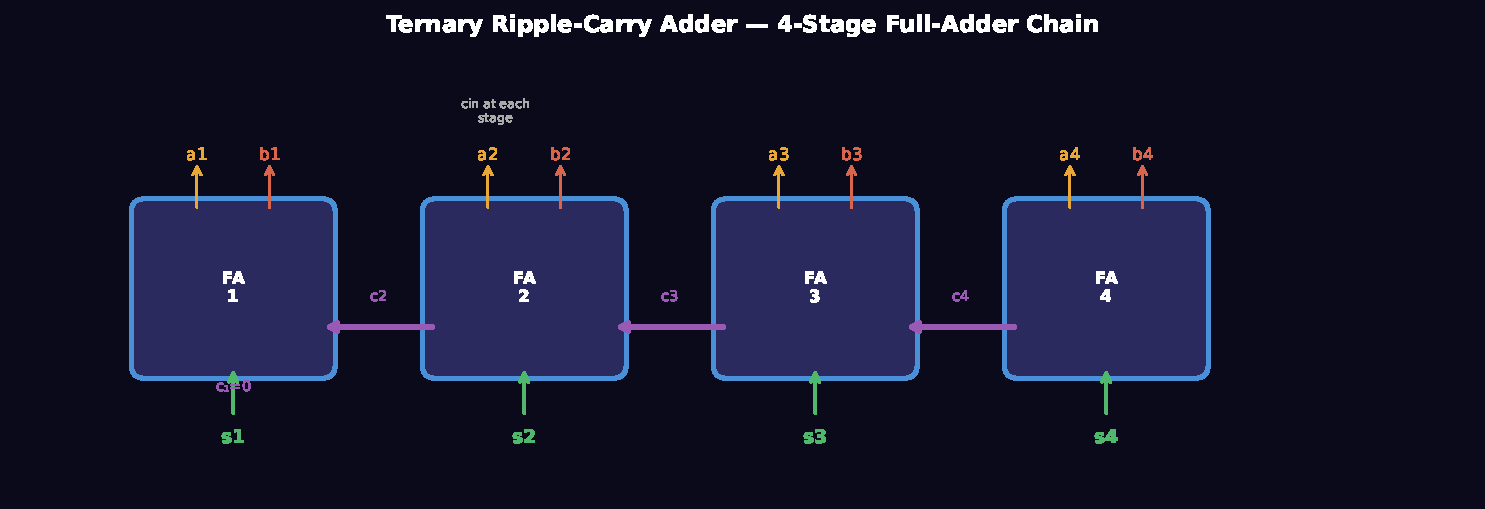
\includegraphics[width=0.62\textwidth]{ripple_carry_adder.pdf}
\caption{Four-stage ternary ripple-carry adder — full adders chained with carry propagation, each summing two operand trits plus carry-in}
\label{fig:rippleadder}
\end{figure}

\subsection{Limitations}

The native adder handles only non-negative strings of digits $\{0,1,2\}$. It does not
support signed numbers, making it unsuitable for general-purpose CPU arithmetic without
additional sign-handling logic.

\section{Decimal Round-Trip}

The CPU ALU uses a fundamentally different approach that naturally handles signed
numbers:

\[
\texttt{add}(a,b) = \texttt{decimal\_to\_ternary}\bigl(
\texttt{ternary\_to\_decimal}(a) + \texttt{ternary\_to\_decimal}(b)\bigr).
\]

This converts both operands to Python integers, performs the arithmetic in the host
environment, and converts the result back to a ternary string. The same pattern extends
to subtraction, multiplication, and division. This method is slower than native ternary
arithmetic but guarantees correctness for all signed values.

%====================================================================
\chapter{Arithmetic via Decimal Round-Trip}
\label{ch:arithmetic}

The \texttt{arithmetic.py} module provides four arithmetic operations, all using the
decimal round-trip approach.

\begin{figure}[H]
\centering
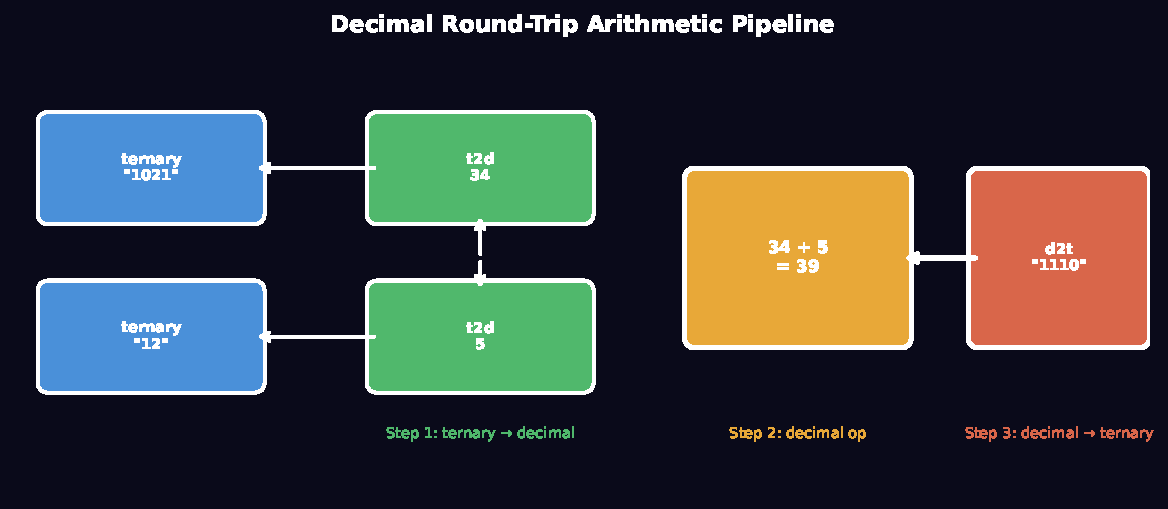
\includegraphics[width=0.72\textwidth]{decimal_roundtrip.pdf}
\caption{Decimal round-trip pipeline — ternary strings are converted to integers, the arithmetic operation is performed in Python, and the result is converted back to ternary}
\label{fig:decroundtrip}
\end{figure}

\subsection*{Addition}
\[
\texttt{add\_ternary}(a,b) = d2t\bigl(t2d(a) + t2d(b)\bigr)
\]

\subsection*{Subtraction}
\[
\texttt{subtract\_ternary}(a,b) = d2t\bigl(t2d(a) - t2d(b)\bigr)
\]
Handles negative results through signed-magnitude encoding.

\subsection*{Multiplication}
\[
\texttt{multiply\_ternary}(a,b) = d2t\bigl(t2d(a) \times t2d(b)\bigr)
\]
Supports negative operands via sign manipulation on the converted integers.

\subsection*{Division}
\[
\texttt{divide\_ternary}(a,b) = d2t\bigl(t2d(a) \mathbin{//} t2d(b)\bigr)
\]
Uses floor division. Raises \texttt{ZeroDivisionError} on division by zero.

The \texttt{validate\_ternary} lambda function ensures all inputs are well-formed before
computation.

\section{Context: When Each Path Is Used}

\begin{table}[H]
\centering
\caption{Addition path usage by context}
\label{tab:addpaths}
\begin{tabular}{ll}
\toprule
Context & Path \\
\midrule
CPU ALU (ADD/SUB/MUL/DIV) & \texttt{arithmetic.py} (decimal round-trip) \\
Educational benchmarks & \texttt{adder.py} (native base-3) \\
PUSH/POP & Memory access (no arithmetic) \\
\bottomrule
\end{tabular}
\end{table}

%====================================================================
\chapter{The Arithmetic Logic Unit}
\label{ch:alu}

The ALU, implemented in \texttt{alu.py}, provides a unified entry point for all
CPU data-processing operations. It dispatches based on an operation code to the
appropriate underlying function.

\section{Supported Operations}

\begin{table}[H]
\centering
\caption{ALU operations}
\label{tab:aluops}
\begin{tabular}{lll}
\toprule
Operation & Function & Implementation \\
\midrule
ADD & $a + b$ & \texttt{arithmetic.add\_ternary} \\
SUB & $a - b$ & \texttt{arithmetic.subtract\_ternary} \\
MUL & $a \times b$ & \texttt{arithmetic.multiply\_ternary} \\
DIV & $a \div b$ & \texttt{arithmetic.divide\_ternary} \\
AND & $\min(a,b)$ & element-wise trit min with padding \\
OR  & $\max(a,b)$ & element-wise trit max with padding \\
NOT & $2 - x$ & trit-wise complement \\
CMP & compare & returns ``EQ'', ``GT'', or ``LT'' \\
\bottomrule
\end{tabular}
\end{table}

\section{Padding for Logical Operations}

For AND and OR, operands may have different lengths. The shorter operand is padded
with leading zeros to match the longer operand's length before element-wise application:
\[
\texttt{pad\_equal\_length}(a,b) =
\begin{cases}
a\text{ padded with }k\text{ leading zeros}, & \text{if } |a| < |b|, \\
b\text{ padded with }k\text{ leading zeros}, & \text{otherwise},
\end{cases}
\]
where $k = \bigl||a| - |b|\bigr|$.

\section{Comparison Flags}

The CMP operation returns a string result (``EQ'', ``GT'', or ``LT'') rather than
modifying registers. The CPU uses this result to set four condition flags:

\begin{table}[H]
\centering
\caption{CMP flag semantics}
\label{tab:cmpflags}
\begin{tabular}{ccccc}
\toprule
Result & ZERO & EQUAL & GREATER & LESS \\
\midrule
dst $=$ src & True & True & False & False \\
dst $>$ src & False & False & True & False \\
dst $<$ src & False & False & False & True \\
\bottomrule
\end{tabular}
\end{table}

Note that ZERO and EQUAL are always set identically by CMP. JZ branches when either
flag is true; JNZ branches only when both are false.

%====================================================================
\chapter{The Register File}
\label{ch:registers}

Trinary provides four general-purpose registers, implemented in \texttt{registers.py}.
The register file is the CPU's fastest storage tier — all arithmetic, logical, and
data movement instructions operate directly on register contents. Memory access
(LOADM/STOREM) is the only mechanism to transfer data between registers and main
memory, imposing a 2-cycle cost on every cross-tier transfer.

\begin{table}[H]
\centering
\caption{Register file specification}
\label{tab:regs}
\begin{tabular}{cll}
\toprule
Register & Encoding (trit) & Convention \\
\midrule
R0 & 0 & Primary accumulator / tensor result TID \\
R1 & 1 & Secondary register \\
R2 & 2 & General purpose \\
R3 & 3 & Always 0 (OS convention) \\
\bottomrule
\end{tabular}
\end{table}

\section{RegisterFile API}

The \texttt{RegisterFile} class provides the following methods:
\begin{description}
    \item[\texttt{load(register, value)}]: Store a ternary string into a register.
          Raises error on invalid register name.
    \item[\texttt{store(register)}]: Return the ternary string value of a register.
    \item[\texttt{move(dst, src)}]: Copy value from source to destination register.
    \item[\texttt{clear(register)}]: Set register to \texttt{"0"}.
    \item[\texttt{dump()}]: Return dictionary of all register values for debugging.
\end{description}

All register values are stored as Python strings (ternary representation). The
\texttt{R3 == "0"} convention is used by the OS shell for efficient zero-comparison.

%====================================================================
\chapter{Memory Architecture}
\label{ch:memory}

The \texttt{Memory} class provides addressable RAM for the CPU. Memory is the second
tier in the storage hierarchy (below CPU registers) and serves as both program store
and data workspace. The CPU loads instructions from the \texttt{program} list (not
directly from memory), but all LOADM/STOREM operations and the PUSH/POP memory stack
interact with the \texttt{Memory} instance.

\begin{figure}[H]
\centering
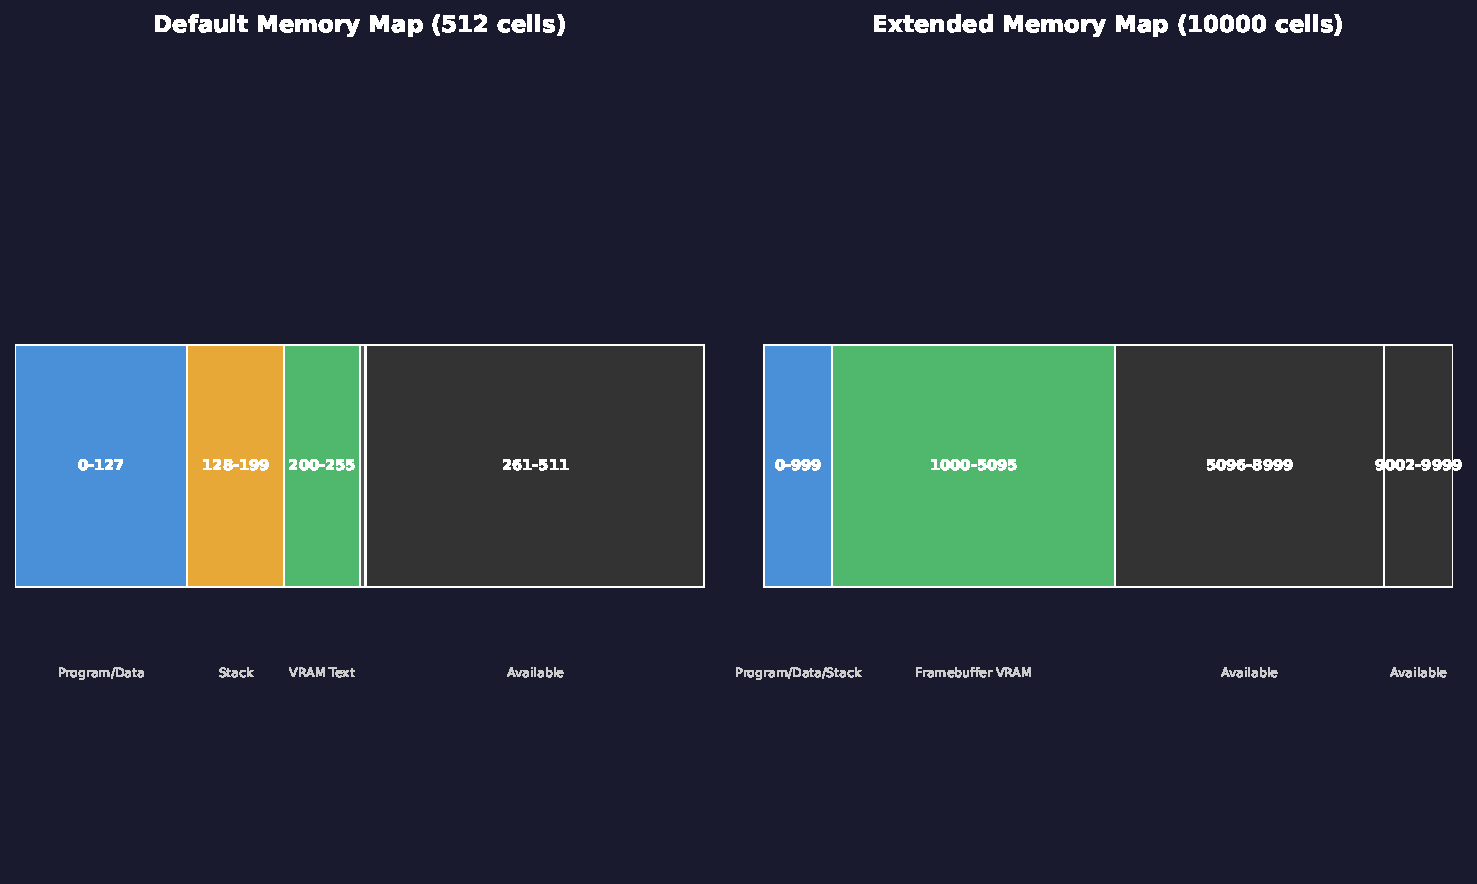
\includegraphics[width=0.68\textwidth]{memory_map.pdf}
\caption{Memory address space layout showing program region, stack, VRAM ranges, and keyboard mapping}
\label{fig:memmap}
\end{figure}

\section{Specification}

\begin{itemize}
    \item Default size: 512 cells (addresses 0--511);
    \item Extended size: 10,000 cells (addresses 0--9999) for SDK framebuffer mode;
    \item Cell contents: ternary strings of variable length;
    \item Storage: Python dictionary for amortised O(1) read/write.
\end{itemize}

\section{Address Space Layout (Default 512-Cell Memory)}

The default memory layout divides the 512 addresses into functional regions:

\begin{table}[H]
\centering
\caption{Default address space layout}
\label{tab:memlayout}
\begin{tabular}{cll}
\toprule
Address Range & Size & Purpose \\
\midrule
0--127 & 128 & Program and data workspace \\
128--199 & 72 & Memory stack (SP starts at 255, grows down to 128) \\
200--255 & 56 & Legacy text-mode VRAM (7$\times$8 character grid) \\
256--259 & 4 & Memory-mapped keyboard status \\
260--511 & 252 & Reserved / extended workspace \\
\bottomrule
\end{tabular}
\end{table}

For the SDK framebuffer configuration (10,000-cell memory), the VRAM range expands to
addresses 1000--5095 (4,096 cells for 64$\times$64 pixel framebuffer) and keyboard
input moves to addresses 9000--9001.

\section{API}

\begin{description}
    \item[\texttt{store(address, value)}]: Write a ternary string to a memory address.
    \item[\texttt{load(address)}]: Read the ternary string at an address.
    \item[\texttt{clear(start, end)}]: Set a range of addresses to \texttt{"0"}.
    \item[\texttt{clear\_all()}]: Reset all memory to \texttt{"0"}.
    \item[\texttt{dump(start, end)}]: Print formatted memory contents.
    \item[\texttt{dump\_hex(start, end)}]: Print hexadecimal representation.
\end{description}

\section{Write Hooks}

A key feature is the write hook mechanism for VRAM synchronization:
\begin{verbatim}
memory.register_write_hook(start, end, callback)
\end{verbatim}

When the CPU writes to any address in the range [start, end], the callback is invoked
automatically. This is used to keep the framebuffer display in sync with CPU memory
writes without polling.

\part{CPU Architecture}

%====================================================================
\chapter{CPU Design: Fetch-Decode-Execute}
\label{ch:cpu}

The CPU, implemented in \texttt{cpu.py}, is the core of the Trinary system. It
implements a classic fetch-decode-execute cycle with 27 opcodes.

\begin{figure}[H]
\centering
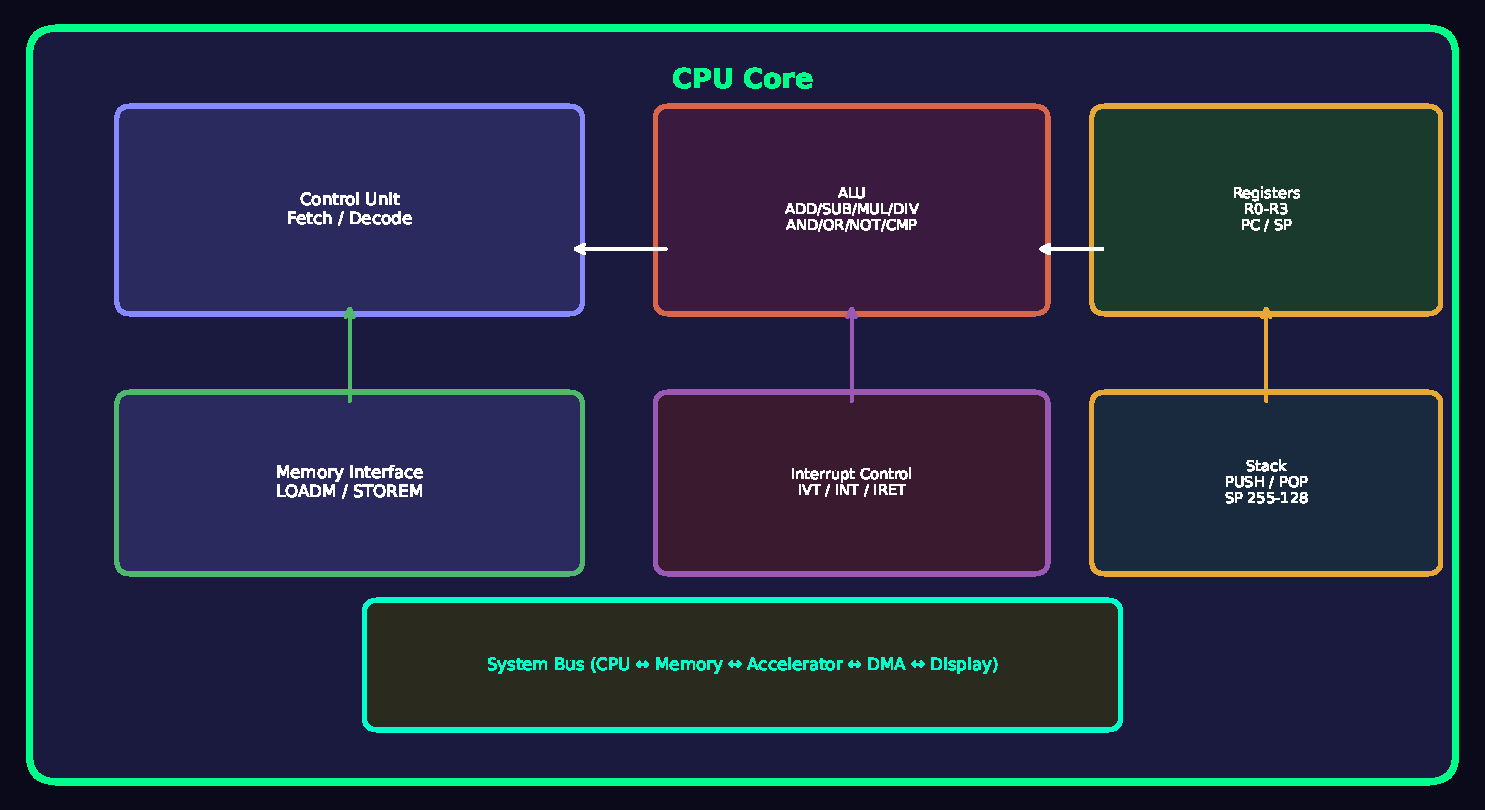
\includegraphics[width=0.72\textwidth]{cpu_architecture.pdf}
\caption{CPU core architecture — control unit, ALU, register file, memory interface, interrupt controller, stack, and system bus}
\label{fig:cpuarch}
\end{figure}

\section{CPU State}

The \texttt{CPU} class maintains:
\begin{itemize}
    \item \textbf{Registers}: R0--R3 via \texttt{RegisterFile};
    \item \textbf{Program Counter (PC)}: integer address of next instruction;
    \item \textbf{Stack Pointer (SP)}: initialized to 255, grows downward;
    \item \textbf{Flags}: ZERO, EQUAL, GREATER, LESS (boolean);
    \item \textbf{Call Stack}: Python list for CALL/RET return addresses;
    \item \textbf{Memory}: \texttt{Memory} instance (default 512, extendable);
    \item \textbf{Program}: list of instruction strings;
    \item \textbf{Interrupt State}: IVT (8 entries), interrupt flag, timer;
    \item \textbf{Optional hardware}: pipeline, cache, bus, DMA, etc.
\end{itemize}

\section{Execution Cycle (Fast Mode)}

In default (instant-execution) mode, each \texttt{step()} call performs:

\begin{enumerate}
    \item \textbf{Fetch}: read $\texttt{program[pc]}$;
    \item \textbf{Decode}: split instruction into opcode and operands via
          \texttt{parse\_instruction()};
    \item \textbf{Execute}: dispatch to the appropriate handler via a 27-branch
          conditional chain;
    \item \textbf{Update}: $\texttt{pc} \gets \texttt{pc} + 1$ (unless the instruction
          modifies PC via branch, call, return, halt, or interrupt);
    \item \textbf{Timer}: $\texttt{timer\_counter} \gets \texttt{timer\_counter}
          - \texttt{CYCLES[opcode]}$;
    \item \textbf{Interrupt check}: if $\texttt{pending} > 0$ and $\texttt{iflag}$
          is true, push PC, jump to $\texttt{IVT[pending]}$, disable interrupts.
\end{enumerate}

\section{Cycle Costs}

Each instruction has an associated cycle cost defined in the \texttt{CYCLES} dictionary.
These costs affect timer-based interrupt timing:

\begin{table}[H]
\centering
\caption{Complete instruction cycle costs}
\label{tab:allcycles}
\begin{tabular}{lcl}
\toprule
Opcode & Cycles & Category \\
\midrule
LOAD, MOV, CLR & 1 & Data movement \\
ADD, SUB, AND, OR, NOT, CMP & 1 & Arithmetic/logic \\
JMP, JZ, JNZ & 1 & Control flow \\
EI, DI, SETIVT, SETTIMER & 1 & System \\
HALT & 1 & System \\
PUSH, POP & 2 & Stack \\
STOREM, LOADM & 2 & Memory \\
INT, IRET & 2 & Interrupts \\
MUL & 3 & Arithmetic \\
CALL, RET & 3 & Subroutines \\
TACT & 3 & Tensor activation \\
TVECADD & 4 & Tensor vector add \\
DIV & 5 & Arithmetic \\
TDOT & 6 & Tensor dot product \\
TLOADW, TSTOREW & 10 & Tensor memory \\
TMATMUL & 20 & Tensor matrix multiply \\
\bottomrule
\end{tabular}
\end{table}

\section{Complete Opcode Map}

The full opcode map assigns a 3-trit ternary opcode to each instruction:

\begin{longtable}{cllllc}
\caption{Complete opcode map (31 opcodes). The Dispatch ID is a sequential identifier, not a ternary-to-decimal conversion of the opcode field.}
\label{tab:opcodelong} \\
\toprule
Ternary & Dispatch ID & Mnemonic & Format & Cycles & Description \\
\midrule
\endfirsthead
\multicolumn{6}{c}{(\emph{continued})} \\
\toprule
Ternary & Dispatch ID & Mnemonic & Format & Cycles & Description \\
\midrule
\endhead
\bottomrule
\endfoot
000 & 0  & LOAD    & C  & 1 & Load immediate into register \\
001 & 1  & MOV     & A  & 1 & Copy register to register \\
002 & 2  & CLR     & B  & 1 & Set register to \texttt{"0"} \\
010 & 3  & ADD     & A  & 1 & Add registers \\
011 & 4  & SUB     & A  & 1 & Subtract registers \\
012 & 5  & AND     & A  & 1 & Ternary AND (element-wise min) \\
020 & 6  & OR      & A  & 1 & Ternary OR (element-wise max) \\
021 & 7  & NOT     & B  & 1 & Ternary NOT (0$\leftrightarrow$2, 1$\rightarrow$1) \\
022 & 8  & CMP     & A  & 1 & Compare, set flags \\
100 & 9  & JMP     & D  & 1 & Unconditional jump \\
101 & 10 & JZ      & D  & 1 & Jump if ZERO or EQUAL \\
102 & 11 & JNZ     & D  & 1 & Jump if NOT ZERO and NOT EQUAL \\
110 & 12 & PUSH    & B  & 2 & Push register to stack \\
111 & 13 & POP     & B  & 2 & Pop register from stack \\
112 & 14 & CALL    & D  & 3 & Call subroutine \\
120 & 15 & RET     & E  & 3 & Return from subroutine \\
121 & 16 & HALT    & E  & 1 & Halt execution \\
122 & 17 & MUL     & A  & 3 & Multiply registers \\
200 & 18 & DIV     & A  & 5 & Divide registers \\
201 & 19 & STOREM  & M  & 2 & Store register to memory \\
202 & 20 & LOADM   & M  & 2 & Load memory into register \\
210 & 28 & TVECADD & A3 & 4 & Tensor vector add, TID$\rightarrow$R0 \\
211 & 29 & TMATMUL & A3 & 20 & Tensor matrix multiply, TID$\rightarrow$R0 \\
212 & 30 & TDOT    & A3 & 6 & Tensor dot product, scalar$\rightarrow$R0 \\
220 & 31 & TACT    & B2 & 3 & Tensor activation in-place (0=step) \\
221 & 32 & TLOADW  & L  & 10 & Load CPU memory into tensor, TID$\rightarrow$R0 \\
222 & 33 & TSTOREW & S2 & 10 & Store tensor to CPU memory \\
\end{longtable}

\section{Instruction Formats}

Each instruction follows a specific encoding pattern:

\begin{table}[H]
\centering
\caption{Instruction encoding formats}
\label{tab:formats}
\begin{tabular}{clll}
\toprule
Format & Pattern & Example & Encoding \\
\midrule
A & OP R\_dst R\_src & ADD R0 R1 & op(3) + dst(1) + src(1) \\
B & OP R\_op & CLR R0 & op(3) + reg(1) \\
C & OP R\_dst value & LOAD R0 10 & op(3) + dst(1) + value(variable) \\
D & OP addr & JMP loop & op(3) + addr(variable) \\
E & OP & HALT & op(3) \\
M & OP addr R\_reg & STOREM 33 R0 & op(3) + reg(1) + addr(variable) \\
A3 & OP dst src\_a src\_b & TVECADD 0 1 2 & op(3) + dst(1) + src\_a(1) + src\_b(1) \\
B2 & OP dst src & TACT 0 0 & op(3) + dst(1) + src(1) \\
L & OP addr rows cols & TLOADW 100 4 4 & op(3) + addr + rows + cols \\
S2 & OP tid addr & TSTOREW 0 100 & op(3) + tid(1) + addr(variable) \\
\bottomrule
\end{tabular}
\end{table}

\begin{figure}[H]
\centering
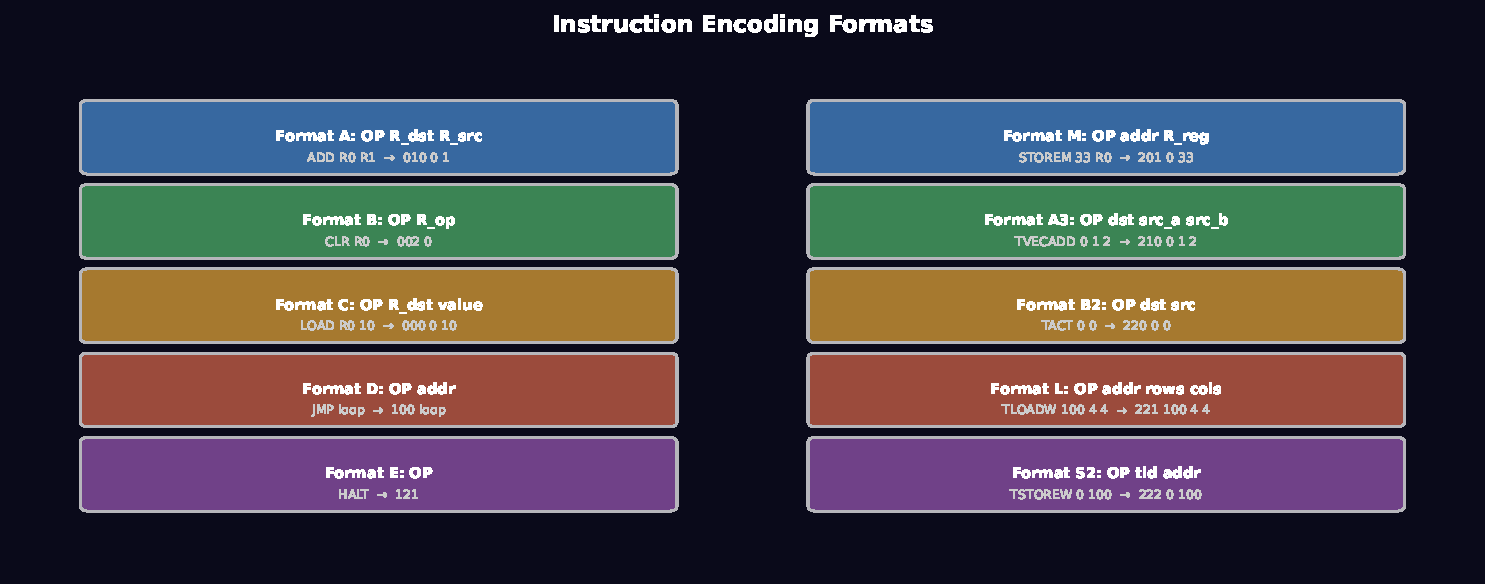
\includegraphics[width=0.68\textwidth]{instruction_formats.pdf}
\caption{All ten instruction encoding formats with examples and ternary representation}
\label{fig:instfmt}
\end{figure}

Register encoding: R0$\rightarrow$0, R1$\rightarrow$1, R2$\rightarrow$2, R3$\rightarrow$3.

\begin{figure}[H]
\centering
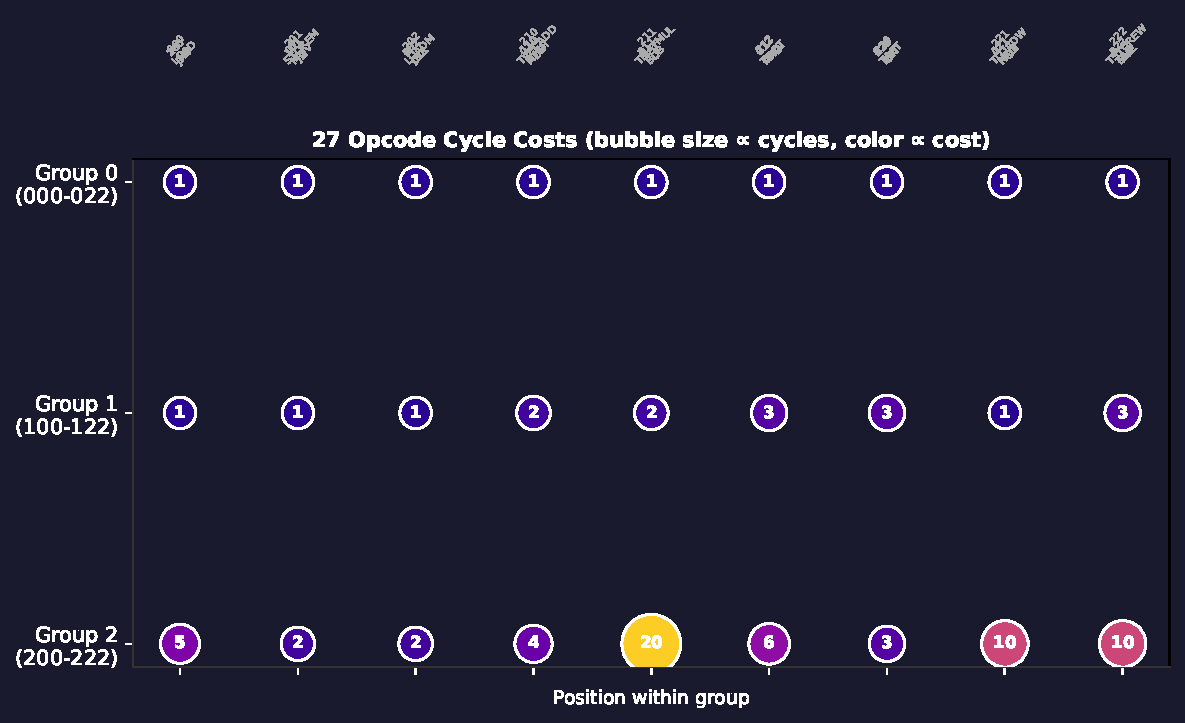
\includegraphics[width=0.72\textwidth]{opcode_heatmap.pdf}
\caption{Opcode distribution heatmap showing instruction categories, cycle costs, and relative usage}
\label{fig:opheat}
\end{figure}

%====================================================================
\chapter{Data Movement Instructions}
\label{ch:datamove}

Data movement instructions transfer ternary values between registers and set
immediate values. They are the most frequently executed instruction class in typical
programs — every computation begins with a LOAD and often ends with a MOV.

\section{LOAD -- Load Immediate}

\begin{verbatim}
LOAD R_dst value
\end{verbatim}
Format C, 1 cycle. Loads the ternary immediate \texttt{value} directly into register
\texttt{R\_dst}. The \texttt{value} is a ternary string literal parsed by the
assembler; it may include a leading minus sign for negative values. No flags are
affected.

\texttt{LOAD} is the primary mechanism for initializing register state. Since there is
no "load from memory address" instruction that doesn't go through a register, all
memory reads begin with \texttt{LOADM} and all arithmetic begins with \texttt{LOAD}.

Example:
\begin{lstlisting}
LOAD R0 10        # R0 = "10" (decimal 3)
LOAD R1 1012      # R1 = "1012" (decimal 32)
LOAD R2 -11       # R2 = "-11" (decimal -4)
\end{lstlisting}

\section{MOV -- Move Register}

\begin{verbatim}
MOV R_dst R_src
\end{verbatim}
Format A, 1 cycle. Copies the value of \texttt{R\_src} to \texttt{R\_dst}. Both
registers must be valid (R0--R3). The source register is unchanged after the copy.
No flags affected.

\texttt{MOV} is essential for preserving values across subroutine calls: a callee
may save incoming arguments by moving them to callee-saved registers before
modifying R0--R3.

\section{CLR -- Clear Register}

\begin{verbatim}
CLR R_dst
\end{verbatim}
Format B, 1 cycle. Sets \texttt{R\_dst} to \texttt{"0"}. Equivalent to
\texttt{LOAD R\_dst 0} but more concise and with a dedicated single-trit encoding.
No flags affected.

\section{Use Cases}

Data movement instructions form the backbone of all Trinary programs:
\begin{itemize}
    \item LOAD initialises loop counters, constants, and memory addresses;
    \item MOV preserves values across operations and rearranges register allocation;
    \item CLR resets accumulators between computation blocks.
\end{itemize}
Together they account for roughly 30--40\% of instructions in typical programs.

%====================================================================
\chapter{Arithmetic and Logical Instructions}
\label{ch:arithlogic}

All arithmetic and logical instructions read both operands, call the ALU, and write
the result to the destination register. Arithmetic instructions (ADD, SUB, MUL, DIV)
set condition flags; logical instructions (AND, OR, NOT) do not. The ALU decodes the
operation string, dispatches to the appropriate handler, and returns a ternary string
result plus flag updates.

\section{Arithmetic Instructions}

\begin{description}
    \item[\texttt{ADD R\_dst R\_src}] (format A, 1 cycle): $R_{dst} \gets
          R_{dst} + R_{src}$. Uses decimal round-trip: both operands are converted
          to integers, summed, and the result is converted back to ternary.
          Sets flags based on the result compared to zero.
    \item[\texttt{SUB R\_dst R\_src}] (format A, 1 cycle): $R_{dst} \gets
          R_{dst} - R_{src}$. Same round-trip mechanism as ADD. Sets flags.
    \item[\texttt{MUL R\_dst R\_src}] (format A, 3 cycles): $R_{dst} \gets
          R_{dst} \times R_{src}$. Multiplication of signed-magnitude ternary strings.
          The higher cycle cost reflects the increased complexity of multi-digit
          multiplication. Sets flags.
    \item[\texttt{DIV R\_dst R\_src}] (format A, 5 cycles): $R_{dst} \gets
          R_{dst} \div R_{src}$. Integer division (floor toward zero). Raises
          \texttt{ZeroDivisionError} on division by zero. The highest cycle cost
          among the core arithmetic operations. Sets flags.
\end{description}

Example -- computing $(3 + 5) \times 5$:
\begin{lstlisting}
LOAD R0 10        # R0 = 3
LOAD R1 12        # R1 = 5
ADD R0 R1         # R0 = 8 (= "22")
MUL R0 R1         # R0 = 40 (= "1111")
\end{lstlisting}

\section{Logical Instructions}

The three logical instructions operate element-wise on ternary digits:

\begin{description}
    \item[\texttt{AND R\_dst R\_src}]: Element-wise minimum $\min(a_i, b_i)$. The
          shorter string is left-padded with \texttt{"0"} before the operation.
          This is the ternary analogue of Boolean AND, where the truth ordering is
          $0 < 1 < 2$.
    \item[\texttt{OR R\_dst R\_src}]: Element-wise maximum $\max(a_i, b_i)$ with
          the same left-padding convention. Ternary analogue of Boolean OR.
    \item[\texttt{NOT R\_dst}]: Trit-wise complement $2 - x_i$ (format B, single
          operand). Maps $0 \leftrightarrow 2$ and leaves $1 \rightarrow 1$.
          This is consistent with the ternary interpretation where 1 is the neutral
          element.
\end{description}

\section{Flag Semantics}

All arithmetic instructions set four condition flags based on the result value:
\begin{itemize}
    \item \textbf{ZERO}: True if the result is \texttt{"0"}.
    \item \textbf{EQUAL}: Same as ZERO for arithmetic results.
    \item \textbf{GREATER}: True if the result represents a positive integer.
    \item \textbf{LESS}: True if the result represents a negative integer.
\end{itemize}
Logical instructions do not modify any flags.

%====================================================================
\chapter{Comparison and Control Flow}
\label{ch:control}

Control flow in Trinary is built on three primitives: comparison (CMP),
unconditional jump (JMP), and conditional jumps (JZ, JNZ). Together they implement
all structured control patterns — if-then, if-else, while, do-while, for, and
infinite loops.

\section{Comparison}

\texttt{CMP R\_dst R\_src} compares two register values and sets four condition flags
(ZERO, EQUAL, GREATER, LESS). The comparison interprets the ternary strings as
decimal integers via conversion. This is the only instruction that modifies flags;
arithmetic instructions set flags only from their result (not from a direct
comparison).

\begin{table}[H]
\centering
\caption{Comparison result truth table}
\label{tab:cmptruth}
\begin{tabular}{lcccc}
\toprule
Condition & ZERO & EQUAL & GREATER & LESS \\
\midrule
$R_{dst} = R_{src}$ & True & True & False & False \\
$R_{dst} > R_{src}$ & False & False & True & False \\
$R_{dst} < R_{src}$ & False & False & False & True \\
\bottomrule
\end{tabular}
\end{table}

\section{Branch Instructions}

\begin{description}
    \item[\texttt{JMP addr}] (format D, 1 cycle): Unconditional jump. Sets
          $\texttt{PC} \gets \texttt{addr}$. Used for loops, tail calls, and
          skip patterns.
    \item[\texttt{JZ addr}] (format D, 1 cycle): Jump if ZERO or EQUAL is True.
          Used after CMP or arithmetic to branch on equality or zero.
    \item[\texttt{JNZ addr}] (format D, 1 cycle): Jump if both ZERO and EQUAL are
          False. Used to continue loops or branch on inequality.
\end{description}

All branch instructions execute in exactly 1 cycle regardless of whether the branch
is taken (format D). The target address is resolved by the two-pass assembler.

Example -- countdown loop:
\begin{lstlisting}
LOAD R0 12        # R0 = 5 (counter)
LOAD R1 1         # R1 = 1 (decrement)
loop:
    SUB R0 R1     # R0 = R0 - 1
    CMP R0 R3     # Compare with 0
    JNZ loop      # Continue if not zero
    HALT
\end{lstlisting}

\section{Pattern: Conditional Execution}

Since there is no conditional-move instruction, conditional logic is expressed
through branch-and-link:
\begin{lstlisting}
LOAD R0 12        # value = 5
LOAD R1 11        # compare = 4
CMP R0 R1         # is value > compare?
JZ skip           # if not, skip
    MOV R2 R0     # R2 = value (only if greater)
skip:
    HALT
\end{lstlisting}

%====================================================================
\chapter{Subroutines: CALL and RET}
\label{ch:subroutines}

Subroutines enable code reuse, modular programming, and structured decomposition of
complex programs. Trinary implements a dual-stack design: CALL/RET use a Python list
(\texttt{call\_stack}) entirely independent from the memory stack used by PUSH/POP.
This separation prevents accidental corruption of return addresses and eliminates the
need for a dedicated link register.

\section{Mechanism}

\begin{description}
    \item[\texttt{CALL addr}] (format D, 3 cycles):
          \begin{enumerate}
              \item Push $\texttt{PC} + 1$ onto \texttt{call\_stack};
              \item Set $\texttt{PC} \gets \texttt{addr}$.
          \end{enumerate}
    \item[\texttt{RET}] (format E, 3 cycles):
          \begin{enumerate}
              \item Pop address from \texttt{call\_stack};
              \item Set $\texttt{PC} \gets \texttt{popped\_addr}$.
          \end{enumerate}
\end{description}

The 3-cycle cost reflects the additional push/pop on the Python call stack. CALL
saves the next instruction address (PC + 1), so execution resumes after the CALL
site when RET executes.

\section{Design Rationale}

The separation of return-address stack from data stack prevents accidental corruption
of return addresses by PUSH/POP operations. In architectures that share a single
stack, a miscalculated POP can corrupt the return address and crash the program.
With the dual-stack design:
\begin{itemize}
    \item The \texttt{call\_stack} contains only return addresses;
    \item The memory stack (SP, addresses 128--255) contains only program data;
    \item A memory stack underflow cannot corrupt the return chain.
\end{itemize}
Nesting is supported to arbitrary depth (limited only by Python's list capacity).
RET on an empty call stack raises \texttt{StackUnderflowError}.

Example:
\begin{lstlisting}
start:
    LOAD R0 10
    CALL func     # Push PC+1, jump to func
    HALT
func:
    ADD R0 R1     # Subroutine body
    RET           # Pop return address, resume at HALT
\end{lstlisting}

\section{Calling Convention}

Trinary uses a simple register-based calling convention:
\begin{itemize}
    \item R0--R2: Argument and return value registers (caller-saved);
    \item R3: Always zero (convention);
    \item Return address is preserved on the \texttt{call\_stack} automatically.
\end{itemize}
Subroutines that modify R0--R2 should save and restore them using the memory stack
(PUSH/POP) if the caller expects preserved values.

%====================================================================
\chapter{Stack Operations: PUSH and POP}
\label{ch:stack}

The memory stack uses the SP register (initialized to 255) and grows downward to a
minimum of 128, providing 128 cells of dedicated stack storage in the default 512-cell
memory configuration.

\section{Mechanism}

\begin{description}
    \item[\texttt{PUSH R\_src}] (format B, 2 cycles):
          \begin{enumerate}
              \item $\texttt{memory[SP]} \gets \texttt{R\_src}$;
              \item $\texttt{SP} \gets \texttt{SP} - 1$.
          \end{enumerate}
          The value is written to the current SP location, then SP is decremented
          (pre-decrement semantics).
    \item[\texttt{POP R\_dst}] (format B, 2 cycles):
          \begin{enumerate}
              \item $\texttt{SP} \gets \texttt{SP} + 1$;
              \item $\texttt{R\_dst} \gets \texttt{memory[SP]}$.
          \end{enumerate}
          SP is first incremented, then the value is read (post-increment semantics).
\end{description}

The 2-cycle cost reflects the memory read/write latency. PUSH and POP are the only
instructions that implicitly access memory (other than LOADM/STOREM).

\section{Error Conditions}

\begin{itemize}
    \item \textbf{Stack overflow}: SP $<$ 128 on PUSH raises
          \texttt{StackOverflowError}. This occurs when the stack has exhausted its
          128-cell region.
    \item \textbf{Stack underflow}: SP $\ge$ 255 on POP raises
          \texttt{StackUnderflowError}. This occurs when POP is called more times
          than PUSH without any intervening stack growth.
\end{itemize}

\section{Typical Usage}

The memory stack is used for three purposes:
\begin{enumerate}
    \item \textbf{Scratch storage}: Temporarily save register values across
          subroutine calls;
    \item \textbf{Interrupt context saving}: The interrupt handler pushes affected
          registers and pops them before IRET;
    \item \textbf{Local variables}: Space can be reserved by decrementing SP
          directly (via SUB on the SP value stored in memory), though this is
          uncommon.
\end{enumerate}

%====================================================================
\chapter{Memory Access Instructions}
\label{ch:memaccess}

STOREM and LOADM provide the interface between the CPU registers and main memory.
They are the only instructions that transfer data across the register--memory boundary
and are therefore critical for all programs that process data beyond the four
registers' capacity.

\begin{description}
    \item[\texttt{STOREM addr R\_src}] (format M, 2 cycles): Write register value
          to memory at the specified address.
    \item[\texttt{LOADM addr R\_dst}] (format M, 2 cycles): Read memory value at
          the specified address into the destination register.
\end{description}

\section{Address Modes}

Both instructions support two addressing modes, distinguished by the operand type:
\begin{itemize}
    \item \textbf{Literal}: \texttt{STOREM 33 R0} — writes R0 to address 33.
          The address is a numeric literal in the assembly source.
    \item \textbf{Register-based}: \texttt{STOREM R2 R0} — writes R0 to the
          address given by the decimal value of register R2. The register value is
          converted to decimal and used as the memory address.
\end{itemize}

The register-based mode enables indexed array access and computed addresses for
data structures. For example, array element access:
\begin{lstlisting}
LOAD R0 10        # R0 = 3 (array index)
LOAD R1 100       # R1 = 100 (array base address)
ADD R1 R0         # R1 = 103 (base + index)
LOADM R1 R2       # R2 = array[index]
\end{lstlisting}

\section{Use in Data Structures}

The STOREM/LOADM pair is the foundation for all memory-resident data structures:
\begin{itemize}
    \item \textbf{Arrays}: Consecutive memory cells accessed via base+offset;
    \item \textbf{Circular buffers}: Used by the snake game body tracker;
    \item \textbf{Frame buffers}: VRAM updates via STOREM to addresses 200--255
          (text mode) or 1000--5095 (framebuffer mode);
    \item \textbf{Memory-mapped I/O}: Keyboard input at address 260 is read via
          LOADM.
\end{itemize}

%====================================================================
\chapter{The Interrupt System}
\label{ch:interrupts}

Trinary provides a full interrupt subsystem with an 8-entry Interrupt Vector Table
(IVT), software and hardware interrupt sources, and nestable interrupt handling.

\section{Interrupt Vector Table}

The IVT has 8 entries (indices 0--7). Each entry stores a handler instruction address.
Entry 0 is used by the hardware timer; entries 1--7 are available for software
interrupts via INT.

\section{Interrupt Instructions}

\begin{description}
    \item[\texttt{EI}] (format E, 1 cycle): Set interrupt flag (enable interrupts).
    \item[\texttt{DI}] (format E, 1 cycle): Clear interrupt flag (disable interrupts).
    \item[\texttt{SETIVT n addr}] (format S, 2 cycles): Set $\texttt{IVT[n]} \gets
          \texttt{addr}$.
    \item[\texttt{INT n}] (format D, 3 cycles): Software interrupt -- push PC+1 to
          stack, disable interrupts, jump to $\texttt{IVT[n]}$.
    \item[\texttt{IRET}] (format E, 3 cycles): Return from interrupt -- pop PC from
          stack, re-enable interrupts.
\end{description}

\section{Interrupt Flow}

When an interrupt fires (either from INT or the timer):
\begin{enumerate}
    \item PC+1 is pushed to the memory stack (using SP);
    \item Interrupts are disabled ($\texttt{iflag} \gets \texttt{False}$);
    \item PC is set to $\texttt{IVT[n]}$, vectoring to the handler;
    \item The handler executes (typically saving/restoring state via STOREM/LOADM);
    \item IRET pops the saved PC and re-enables interrupts.
\end{enumerate}

\begin{figure}[H]
\centering
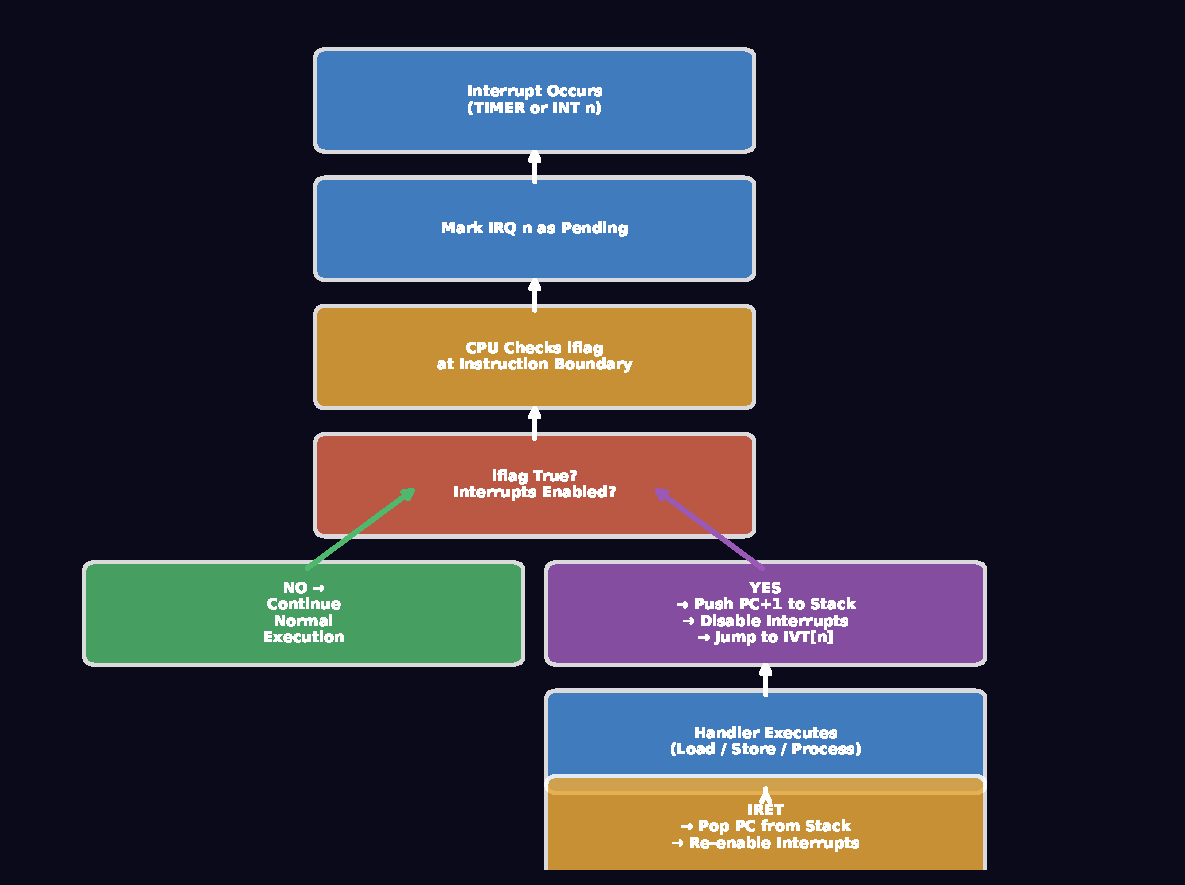
\includegraphics[width=0.62\textwidth]{interrupt_flow.pdf}
\caption{Interrupt handling flow — from trigger through vectoring, handler execution, and IRET return}
\label{fig:intflow}
\end{figure}

This sequence prevents re-entrancy during handler execution.

%====================================================================
\chapter{Timer and Interrupt-Driven Execution}
\label{ch:timer}

The hardware timer enables periodic interrupt generation for preemptive multitasking
and real-time event handling. It is the CPU's only source of hardware-triggered
interrupts (software interrupts are generated via the INT instruction).

\section{Timer Mechanism}

\begin{description}
    \item[\texttt{SETTIMER period}] (format T, 1 cycle): Set $\texttt{timer\_period}
          \gets \texttt{period}$ and $\texttt{timer\_counter} \gets \texttt{period}$.
          The period is measured in CPU cycles.
\end{description}

After SETTIMER, each CPU \texttt{step()} decrements the timer counter by the executed
instruction's cycle cost. When $\texttt{timer\_counter} \le 0$:
\begin{enumerate}
    \item Interrupt 0 is marked as pending;
    \item $\texttt{timer\_counter} \gets \texttt{timer\_period}$ (auto-reload);
    \item On the next instruction boundary, if $\texttt{iflag}$ is True, the CPU
          vectors to $\texttt{IVT[0]}$.
\end{enumerate}

\section{Timing Accuracy}

Timer accuracy depends on instruction cycle costs. Since instructions have different
cycle counts (1--20), the timer decrements by the exact cost of each executed
instruction rather than by 1 per step. This means:
\begin{itemize}
    \item A loop of 1-cycle instructions (LOAD, ADD, JMP) experiences interrupts at
          precise intervals;
    \item A loop containing a DIV (5 cycles) or TMATMUL (20 cycles) stretches the
          interval proportionally;
    \item The timer counter can underflow by more than 1 if a multi-cycle instruction
          crosses the boundary, but the auto-reload mechanism ensures the next period
          starts from \texttt{timer\_period} regardless.
\end{itemize}

\section{Preemptive Multitasking Pattern}

The timer interrupt can be used to implement cooperative or preemptive multitasking:

\begin{lstlisting}
SETIVT 0 scheduler    # Timer ISR → task scheduler
EI                    # Enable interrupts
SETTIMER 100          # Schedule every 100 cycles

task1:
    # Task 1 code
    JMP task1

task2:
    # Task 2 code
    JMP task2

scheduler:
    # Context switch logic
    # Save current task state to memory
    # Load next task state from memory
    IRET
\end{lstlisting}

\section{Example: Timer-Driven Counter}

\begin{lstlisting}
SETIVT 0 handler      # Set up timer handler at 'handler'
EI                    # Enable interrupts
SETTIMER 50           # Fire interrupt 0 every 50 cycles

main_loop:
    LOAD R0 1
    ADD R0 R0
    JMP main_loop

handler:
    LOADM 100 R0      # Load tick counter
    LOAD R1 1
    ADD R0 R1
    STOREM 100 R0     # Save tick counter
    IRET              # Return from interrupt
\end{lstlisting}

\section{Practical Considerations}

\begin{itemize}
    \item The handler must be short: long handler execution delays the main program.
    \item Interrupts are disabled during handler execution; nested interrupts are
          possible only if the handler explicitly re-enables them via EI.
    \item The SETTIMER period should account for worst-case handler execution time
          to avoid interrupt storms (back-to-back timer triggers).
    \item Timer-driven scheduling is validated by integration tests in
          \texttt{test\_realistic\_cpu.py} and unit tests in \texttt{test\_interrupts.py}.
\end{itemize}

\part{Toolchain}

%====================================================================
\chapter{The Two-Pass Assembler}
\label{ch:assembler}

The assembler (\texttt{assembler.py}) translates symbolic assembly language into
instruction strings for the CPU. It uses a two-pass design to handle forward references.

\begin{figure}[H]
\centering
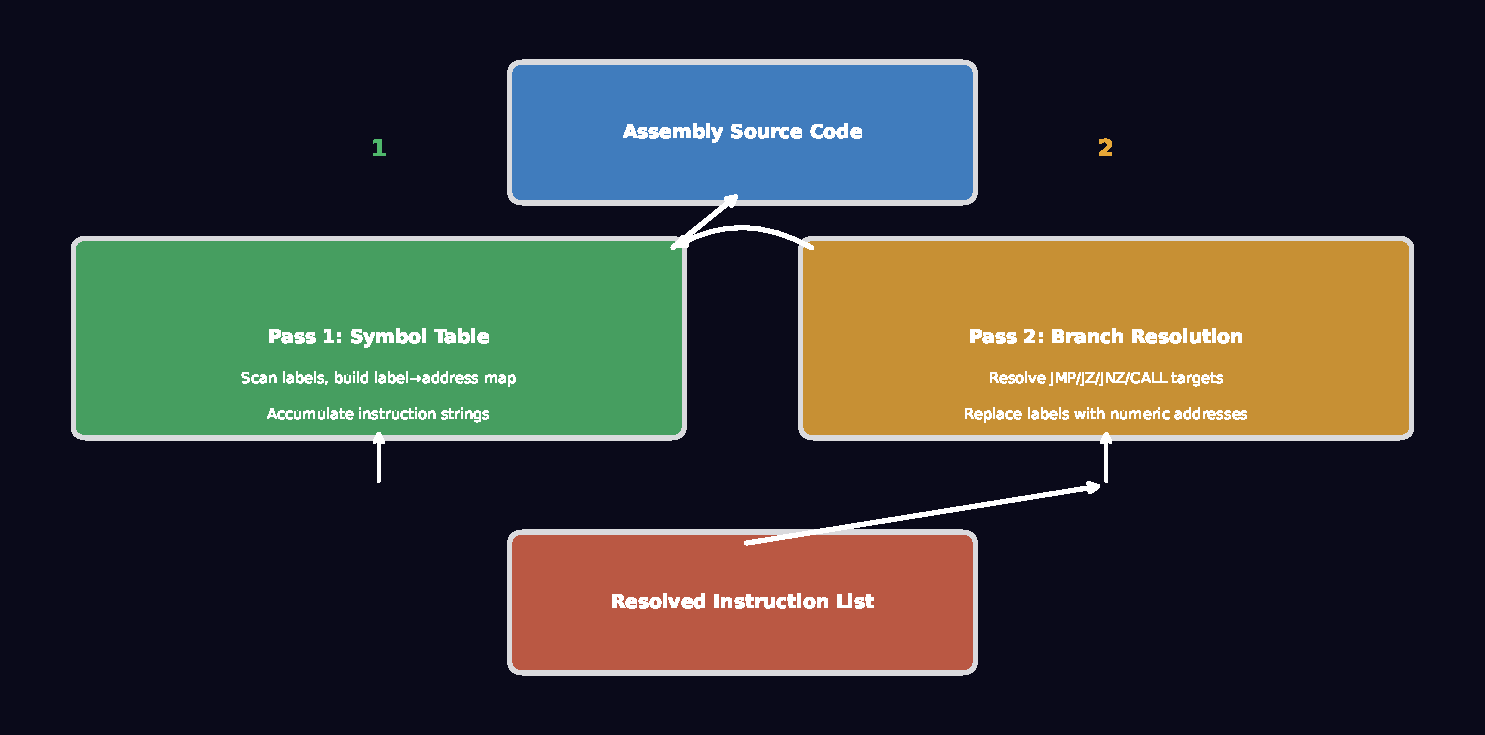
\includegraphics[width=0.72\textwidth]{assembler_flow.pdf}
\caption{Two-pass assembler flow — Pass 1 builds the symbol table, Pass 2 resolves forward branch references}
\label{fig:asmflow}
\end{figure}

\section{Assembly Syntax}

\begin{verbatim}
label:
    OPCODE operand operand  # inline comment
    OPCODE operand          ; also a comment
\end{verbatim}

Labels are identifiers followed by a colon. They serve as branch targets and CALL
addresses. Two comment delimiters are supported: \texttt{\#} and \texttt{;}.

\section{Pass 1: Symbol Table Construction}

The first pass scans each source line:
\begin{enumerate}
    \item Strip comments and whitespace;
    \item If line contains a label (\texttt{name:}), record $\texttt{label\_name}
          \rightarrow \texttt{current\_address}$ in the symbol table;
    \item Increment address for each non-label, non-comment line;
    \item Accumulate instruction strings for the program listing.
\end{enumerate}

\section{Pass 2: Branch Resolution}

The second pass processes each instruction:
\begin{enumerate}
    \item For branch opcodes (JMP, JZ, JNZ, CALL), check if the operand is a label;
    \item If so, look up the label's address in the symbol table and replace the
          operand;
    \item If the label is not found, raise an error.
\end{enumerate}

This produces a clean list of instruction strings with all label references resolved
to numeric addresses.

%====================================================================
\chapter{Machine Code Encoding and Decoding}
\label{ch:machine}

The machine-code encoder (\texttt{machine.py}) converts assembly instruction strings
to and from variable-length ternary opcode strings.

\section{Encoder}

\texttt{encode\_instruction(instruction)} parses the assembly string and produces a
ternary machine-code string according to the instruction format:

\begin{itemize}
    \item Format A (\texttt{OP dst src}): $\texttt{opcode}(3) + \texttt{dst}(1) +
          \texttt{src}(1)$
    \item Format B (\texttt{OP reg}): $\texttt{opcode}(3) + \texttt{reg}(1)$
    \item Format C (\texttt{OP dst value}): $\texttt{opcode}(3) + \texttt{dst}(1) +
          \texttt{value}(\text{variable})$
    \item Format D (\texttt{OP addr}): $\texttt{opcode}(3) + \texttt{addr}(\text{variable})$
    \item Format E (\texttt{OP}): $\texttt{opcode}(3)$
    \item Format M (\texttt{OP addr reg}): $\texttt{opcode}(3) + \texttt{reg}(1) +
          \texttt{addr}(\text{variable})$
\end{itemize}

Example encoding:
\begin{lstlisting}
LOAD R0 10        → 000010
ADD R0 R1         → 01001
HALT              → 121
STOREM 33 R0      → 20101020
\end{lstlisting}

\section{Decoder}

\texttt{decode\_instruction(machine\_code)} performs the reverse transformation,
parsing the ternary string according to the known format and reconstructing the
assembly instruction.

\section{Unmapped Instructions}

The following instructions have no ternary encoding and are executed directly from
their assembly representation: INT, IRET, EI, DI, SETIVT, SETTIMER. This is because
they are system-control instructions that are typically generated by the assembler
rather than by user code, and their variable-length operand formats make fixed
encoding impractical.

%====================================================================
\chapter{The TAL Compiler}
\label{ch:tal}

TAL (Ternary Assembly Language) is a structured high-level language that compiles to
ternary CPU assembly. It provides variables, constants, control flow, and drawing
primitives.

\begin{figure}[H]
\centering
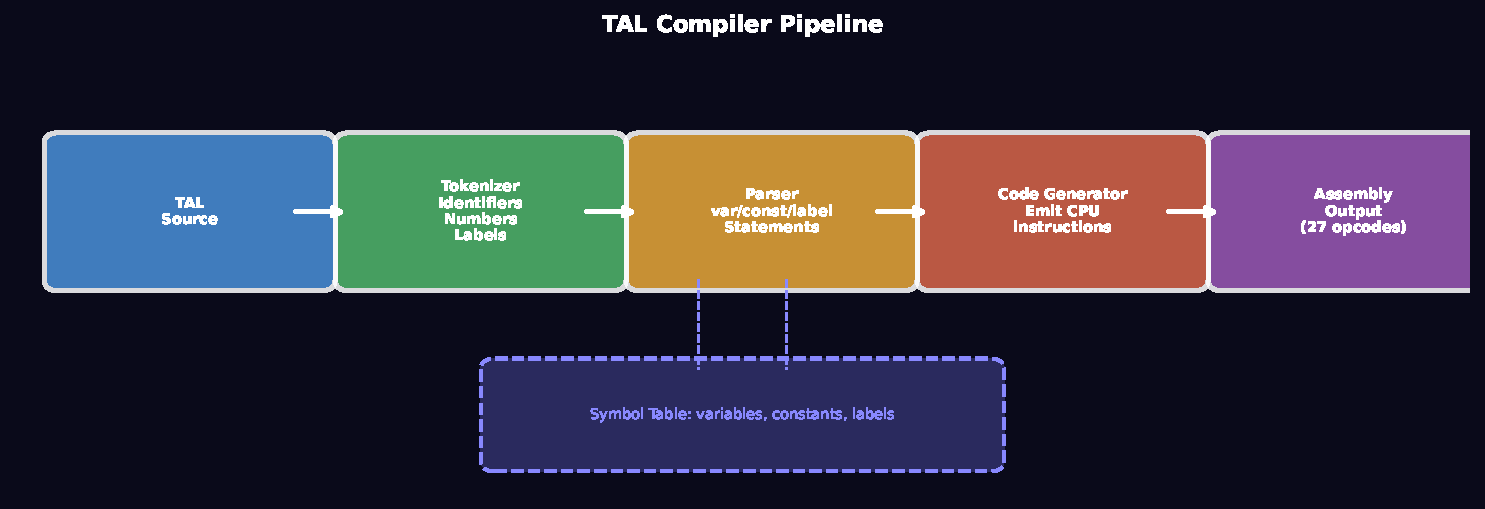
\includegraphics[width=0.72\textwidth]{tal_pipeline.pdf}
\caption{TAL compiler pipeline — tokenizer, parser, symbol table, and code generator produce CPU assembly output}
\label{fig:talcpl}
\end{figure}

\section{Language Syntax}

\begin{verbatim}
var name @address       # Declare variable at memory address
const name = value      # Declare named constant
label name:             # Define label (or 'name:' alone)

# Statements:
store var, value        # Store value into variable
load var, addr          # Load from address into variable
inc var                 # Increment variable
dec var                 # Decrement variable
add dst, a, b           # dst = a + b
sub dst, a, b           # dst = a - b
if_eq a, b, label       # Branch to label if a == b
if_ne a, b, label       # Branch to label if a != b
draw x, y, color        # Set pixel on framebuffer
clear x, y              # Clear pixel on framebuffer
write addr, value       # Write value to memory address
jmp label               # Unconditional jump
halt                    # Stop execution
\end{verbatim}

\section{Compilation Flow}

The compiler operates in a single pass:
\begin{enumerate}
    \item Tokenize the TAL source into statements;
    \item Parse variable and constant declarations into a symbol table;
    \item Process each statement, emitting CPU assembly instructions with resolved
          addresses.
\end{enumerate}

Address constants use \texttt{@addr} notation, which is resolved during compilation.
Variables declared with \texttt{var counter @100} are mapped to memory address 100.

\section{Snake Game}

The most significant TAL program is a complete Snake game (\texttt{snake\_game.py}),
consisting of 524 TAL-compiled CPU instructions. The snake body is stored in a
circular buffer at memory addresses 20--147. The \texttt{TALSnake} class provides
\texttt{init()}, \texttt{update()}, \texttt{render()}, and \texttt{shutdown()}
methods, forming a drop-in replacement for the pure-Python \texttt{CPUSnake}
implementation.

\part{Software Environment}

%====================================================================
\chapter{Memory-Mapped Display and Keyboard}
\label{ch:display}

Trinary provides two independent display subsystems that can be used separately or
simultaneously.

\begin{table}[H]
\centering
\caption{Dual display subsystem specifications}
\label{tab:displays}
\begin{tabular}{llll}
\toprule
Layer & VRAM Range & Resolution & Keyboard \\
\midrule
Legacy (text) & 200--255 & 7 $\times$ 8 chars (56 chars) & Address 260 \\
SDK (framebuffer) & 1000--5095 & 64 $\times$ 64 pixels (4096 px) & Addresses 9000--9001 \\
\bottomrule
\end{tabular}
\end{table}

\section{Legacy Text Display}

VRAM addresses 200--255 store the ternary encoding of ASCII character codes. The
\texttt{DisplayMemoryMap} class converts each cell to a character via
$\texttt{chr}(\texttt{ternary\_to\_decimal}(\texttt{value}))$ and arranges them
in a 7-row $\times$ 8-column grid.

\subsection{Character Addressing}

The 56-character grid is addressed linearly: position 0 is the top-left corner,
position 7 the top-right, position 56 is the bottom-left, and position 55 the
bottom-right. Row--column to address mapping:
\[
\texttt{vram\_addr} = 200 + \texttt{row} \times 8 + \texttt{col}.
\]

\subsection{Rendering Rules}

\begin{itemize}
    \item Value \texttt{"0"} renders as a space (empty cell).
    \item Non-printable characters (ASCII codes 0--31) render as \texttt{'.'}.
    \item Printable ASCII (codes 32--126) renders as the corresponding character.
    \item Extended codes (127+) render as \texttt{'?'}.
\end{itemize}

Example -- writing ASCII 'H' to VRAM grid position (row 0, column 0):
\begin{lstlisting}
LOAD R1 2200       # R1 = ternary for ASCII 72 (ord('H'))
STOREM 200 R1      # VRAM[200] = 'H' (top-left)
\end{lstlisting}

\section{SDK Framebuffer Display}

The framebuffer uses 4,096 VRAM cells mapped to a 64 $\times$ 64 pixel grid via:
\[
\texttt{address} = 1000 + y \times 64 + x.
\]

\subsection{Pixel Addressing}

Pixel $(x, y)$ corresponds to VRAM address $1000 + y \times 64 + x$ where
$x \in [0, 63]$ and $y \in [0, 63]$. The 64-byte row stride matches the display
width, enabling efficient row-wise operations. A single row fill requires 64
consecutive STOREM instructions.

\subsection{Dirty-Rect Tracking}

The \texttt{Framebuffer} class maintains a dirty rectangle that tracks the
minimal bounding box of all modified pixels since the last \texttt{clear\_dirty()}
call:
\begin{verbatim}
dirty = (min_x, min_y, max_x, max_y)
\end{verbatim}
On each render cycle, only the dirty region is re-drawn, reducing PyQt6 redraw
overhead by up to 90\% in typical game workloads.

Each cell stores a palette index (0--8) selecting from 9 colors:

\section{Keyboard Input}

Two keyboard interfaces exist:

\paragraph{Legacy (address 260):} The CPU reads \texttt{LOADM 260 R1} to poll. A
non-zero value indicates a key waiting. After processing, the CPU writes \texttt{"0"}
to acknowledge.

\paragraph{SDK (addresses 9000--9001):} Address 9000 holds the ASCII code of the last
key pressed; address 9001 holds a status flag (1 = key waiting, 0 = no key). The SDK
input API provides \texttt{btn(name)} and \texttt{btnp(name)} with 8-button D-pad
mapping.

\section{Write Hooks}

The \texttt{Memory} class supports write hooks for automatic framebuffer
synchronization:
\begin{verbatim}
memory.register_write_hook(1000, 5095, callback)
\end{verbatim}
When the CPU writes to any address in the framebuffer VRAM range, the callback fires
automatically, keeping the display up to date without polling.

%====================================================================
\chapter{The Operating System Shell}
\label{ch:os}

Two OS implementations coexist in Trinary, serving different display subsystems and
use cases.

\section{Legacy OS (\texttt{os.py})}

A 342-instruction assembly program (generated by the \texttt{\_gen()} function)
implementing an interactive TTY shell:

\begin{description}
    \item[\textbf{Boot sequence}:] Clear display, print ``Trishell!'' banner, show
          prompt;
    \item[\textbf{Main loop}:] Poll keyboard (address 260), classify key, echo to
          display, process backspace and enter;
    \item[\textbf{Commands}:] HELP, CLS, REGS, MEMDUMP, RUN;
    \item[\textbf{Input buffer}:] Addresses 1--32, with backspace support.
\end{description}

The legacy OS memory map:
\begin{table}[H]
\centering
\caption{Legacy OS memory layout}
\label{tab:osmem}
\begin{tabular}{cl}
\toprule
Address & Purpose \\
\midrule
0 & Cursor offset (0--55) \\
1--32 & Input buffer \\
33 & Input buffer length \\
200--255 & VRAM (display) \\
260 & Keyboard buffer \\
\bottomrule
\end{tabular}
\end{table}

\section{Modular SDK OS (\texttt{os/} package)}

A Python package providing a richer operating environment:

\begin{table}[H]
\centering
\caption{SDK OS module structure}
\label{tab:sdkos}
\begin{tabular}{ll}
\toprule
Module & Purpose \\
\midrule
\texttt{kernel.py} & OS kernel, boot sequence, main loop \\
\texttt{shell.py} & Command dispatch and parsing \\
\texttt{terminal.py} & Input buffer, cursor, scrolling \\
\texttt{syscalls.py} & System call interface \\
\texttt{commands.py} & Built-in command registry \\
\texttt{text\_renderer.py} & 8$\times$8 bitmap font rendering \\
\texttt{boot.py} & Boot splash and initialization \\
\texttt{program\_loader.py} & Load and verify assembly programs \\
\texttt{constants.py} & VERSION, COLORS, etc. \\
\bottomrule
\end{tabular}
\end{table}

\subsection{SDK OS Commands}

\begin{description}
    \item[\texttt{HELP}]: Lists all available commands with brief descriptions.
    \item[\texttt{CLS}]: Clears the terminal display and resets cursor position.
    \item[\texttt{MEM}]: Dumps memory contents in a formatted hex view (address range
          can be specified).
    \item[\texttt{REGS}]: Displays all CPU register values (R0--R3, PC, SP, flags).
    \item[\texttt{CLEAR}]: Resets CPU and memory to initial state.
    \item[\texttt{ABOUT}]: Shows version information and system statistics.
    \item[\texttt{DEMO}]: Loads and runs a built-in demo program by name.
    \item[\texttt{RUN}]: Executes a user-supplied assembly program from the terminal.
    \item[\texttt{HALT}]: Stops CPU execution and returns to the shell prompt.
    \item[\texttt{CPU}]: Shows CPU configuration, cycle count, and performance metrics.
\end{description}

\subsection{Kernel Architecture}

The \texttt{Kernel} class manages the boot sequence and main execution loop:
\begin{enumerate}
    \item \textbf{Boot}: Clears memory, initialises the terminal, mounts the program
          registry, displays the splash screen.
    \item \textbf{Main loop}: Reads keyboard input via the terminal, dispatches
          commands through the shell parser, executes the requested command or
          programs, and returns to the prompt.
    \item \textbf{Program loading}: The \texttt{program\_loader} module verifies
          assembly syntax, assembles the code, and loads it into CPU memory starting
          at address 0. Errors are reported back to the terminal.
    \item \textbf{Text rendering}: The \texttt{text\_renderer} module uses an
          8$\times$8 bitmap font stored in a lookup table, enabling proportionally
          spaced character output on the 64$\times$64 framebuffer.
\end{enumerate}

Both OS paths are validated by 38 integration tests in \texttt{test\_os.py}.

%====================================================================
\chapter{The PyQt6 Visual Simulator}
\label{ch:ui}

The desktop UI (\texttt{src/trinary/ui/}) provides a comprehensive visual debugging
environment, built with PyQt6.

\begin{figure}[H]
\centering
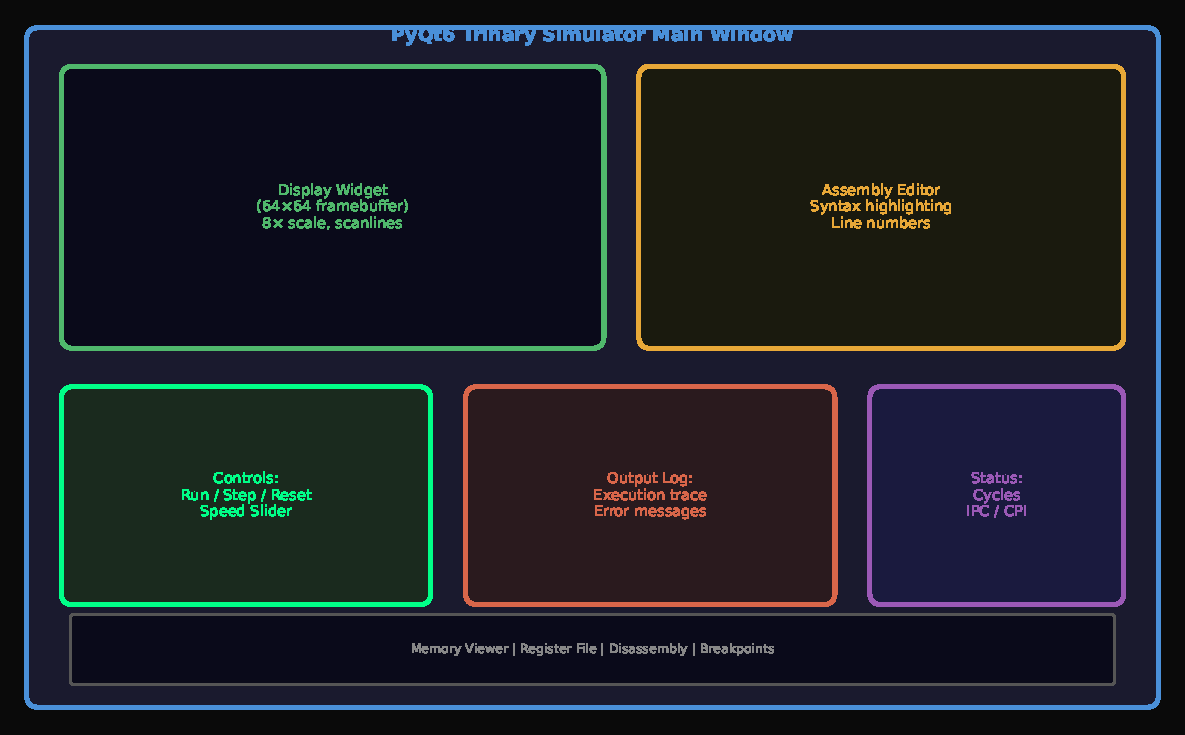
\includegraphics[width=0.72\textwidth]{simulator_gui.pdf}
\caption{PyQt6 simulator window layout — display widget, assembly editor, controls, output log, status panel, and memory/register viewers}
\label{fig:simgui}
\end{figure}

\section{Widgets}

The main window assembles 17 panels in a splitter layout:
\begin{enumerate}
    \item \textbf{Assembly Editor}: Syntax highlighting (cyan opcodes, yellow registers,
          purple labels, green comments), gutter breakpoints;
    \item \textbf{Machine Code Viewer}: Side-by-side assembly and ternary opcodes;
    \item \textbf{Register/Flag Inspector}: Flash animation on value change;
    \item \textbf{Memory Viewer}: 512-row table with read (blue) and write (green)
          access tracking;
    \item \textbf{Stack Viewer}: SP position with live item list;
    \item \textbf{Execution Trace}: Step-by-step history (PC, instruction, registers,
          flags);
    \item \textbf{Pipeline Widget}: 5-stage IF$\rightarrow$ID$\rightarrow$EX$\rightarrow$MEM$\rightarrow$WB
          occupancy visualization;
    \item \textbf{Cache Widget}: Direct-mapped L1 contents and hit/miss counters;
    \item \textbf{Bus Widget}: Transaction log with arbitration events;
    \item \textbf{Branch Widget}: 2-bit predictor state and accuracy percentage;
    \item \textbf{Performance Dashboard}: CPI, IPC, cache hit rate, branch accuracy;
    \item \textbf{Timeline Viewer}: Cycle-by-cycle instruction trace;
    \item \textbf{Waveform Viewer}: Signal transition visualization;
    \item \textbf{Game Window}: 64 $\times$ 64 framebuffer at 8$\times$ scale;
    \item \textbf{Debugger Panel}: Run/Step/Continue with breakpoint management.
\end{enumerate}

\section{Controls}

Toolbar: demo selector, Assemble, Run, Step Into, Reset, Pause, Continue.

\section{Theme}

Dark cyberpunk aesthetic: background \texttt{\#0a0a0f}, green text \texttt{\#00ff88},
cyan opcodes \texttt{\#00ffff}, yellow registers \texttt{\#ffff00}, purple labels
\texttt{\#aa66ff}.

%====================================================================
\chapter{Games and Demos}
\label{ch:games}

\section{Legacy CPU Demos}

\texttt{demo\_programs.py} provides 13 assembly programs running on the ternary CPU
with the 7$\times$8 text display:

\begin{itemize}
    \item \textbf{Countdown}: Decrements from 9 to 0, displaying each value on the
          character grid. Demonstrates basic LOAD/SUB/CMP/JNZ loop structure.
    \item \textbf{Fibonacci}: Computes and displays Fibonacci numbers up to 987
          (the 16th term). Demonstrates register-to-register moves and multi-cycle
          arithmetic sequences.
    \item \textbf{Factorial}: Computes $n!$ iteratively. Demonstrates MUL with
          accumulator patterns.
    \item \textbf{Sum 1 to N}: Accumulates integers from 1 to a user-supplied $N$.
    \item \textbf{Calculator}: Accepts two operands and an operator via keyboard input,
          performs the operation, and displays the result. Demonstrates keyboard I/O
          with interrupt-driven input processing.
    \item \textbf{Timer Interrupt}: Uses SETTIMER and SETIVT to generate periodic
          interrupts. The handler updates a display counter. Demonstrates timer-driven
          preemption.
    \item \textbf{Pixel Diagonal}: Draws a diagonal line across the 27$\times$27
          PixelDisplay using Bresenham's line algorithm. Demonstrates memory-to-memory
          data movement and computational geometry.
    \item \textbf{Keyboard Echo}: Reads keyboard input from address 260 and echoes
          characters to the text display. Demonstrates polling-based I/O.
\end{itemize}

These 13 programs serve as both functional tests and introductory teaching examples.

\section{SDK Games}

\texttt{demo\_games.py} provides 8 graphical games using the Fantasy Console SDK.
Each game runs at 30 FPS on the 64$\times$64 framebuffer and is driven by the
\tt{Engine} + \tt{Runtime} framework:

\begin{enumerate}
    \item \textbf{Pong}: Two-player paddle-ball game with left/right D-pad controls
          and on-screen score tracking. Ball physics include angle-dependent reflection
          off paddles and wall bouncing. First player to 5 wins.
    \item \textbf{Snake Deluxe}: TAL-compiled snake game (524 CPU instructions). The
          snake body is stored in a circular buffer at memory addresses 20--147.
          The head moves continuously; the player steers with D-pad. Eating food
          grows the body and increments the score. Collision with walls or self
          ends the game. This is the most complex TAL-compiled program.
    \item \textbf{Breakout}: Brick-breaking game with a 7$\times$4 grid of destructible
          bricks. Ball physics include paddle collision, wall bouncing, and brick
          removal. The paddle is controlled via LEFT/RIGHT. The game tracks score
          and remaining lives.
    \item \textbf{Particles}: 50-particle fountain effect with simulated gravity
          ($v_y \gets v_y + 0.3$ per frame). Each particle has a 30-frame lifetime
          and a randomized color from the 9-color palette. Particles are recycled
          upon death, producing a continuous fountain. Demonstrates array-based
          particle systems on the ternary platform.
    \item \textbf{Pixel Paint}: Freeform drawing on the 64$\times$64 canvas. The
          player moves a cursor with the D-pad and draws with the action button.
          Demonstrates framebuffer pixel manipulation and real-time input handling.
    \item \textbf{Bouncing Logo}: A rect-within-rect animation bouncing at 45$^\circ$
          off screen boundaries. Demonstrates physics-free animation and framebuffer
          compositing.
    \item \textbf{Tilemap Scroller}: A scrollable 32$\times$32 tile world viewed
          through the 64$\times$64 camera window. The camera follows player input.
          Demonstrates tile-based world rendering with camera offset.
    \item \textbf{RPG Movement}: A 16$\times$16 tile world with collision detection
          and camera-follow. The player moves through a predefined map with
          impassable tiles. Demonstrates grid-based movement, collision, and
          scrolling camera.
\end{enumerate}

\section{Running Demos}

Demos are launched via the unified runner:
\begin{verbatim}
python -m trinary.demo_games pong
python -m trinary.demo_games snake
python -m trinary.demo_games breakout
python -m trinary.demo_games particles
python -m trinary.demo_games paint
python -m trinary.demo_games bouncing_logo
python -m trinary.demo_games tilemap
python -m trinary.demo_games rpg
\end{verbatim}

Each demo supports \texttt{--help} for additional command-line options.

%====================================================================
\chapter{The TAL Compiler (Extended)}
\label{ch:tal-ext}

This chapter provides additional implementation details for the TAL compiler introduced
in Chapter~\ref{ch:tal}.

\section{Compiler Architecture}

The compiler operates in a single pass:
\begin{enumerate}
    \item \textbf{Tokenizer}: Splits the source into tokens (identifiers, numbers,
          operators, labels, directives);
    \item \textbf{Symbol Table}: Maintains mappings for variables ($\texttt{name}
          \rightarrow \texttt{address}$), constants ($\texttt{name} \rightarrow
          \texttt{value}$), and labels ($\texttt{name} \rightarrow \texttt{assembly
          address}$);
    \item \textbf{Code Generator}: Emits CPU assembly instructions for each TAL
          statement, using the symbol table to resolve references.
\end{enumerate}

\section{Compilation Examples}

TAL source:
\begin{verbatim}
var counter @100
const MAX = 10
label start:
    store counter, 0
label loop:
    if_eq counter, MAX, done
    inc counter
    jmp loop
label done:
    halt
\end{verbatim}

Compiles to approximately 15 CPU instructions including LOAD, STOREM, LOADM, CMP, JZ,
ADD, JMP, and HALT.

\section{Array Access}

Circular buffer access (\texttt{body\_x[head]}) compiles to a multi-instruction
sequence:
\begin{enumerate}
    \item Load \texttt{head} into a register;
    \item Add the base address of \texttt{body\_x};
    \item Use the computed address with LOADM/STOREM.
\end{enumerate}

This enables efficient circular buffer manipulation for the snake game's body tracking.

%====================================================================
\chapter{The Dual Display System}
\label{ch:dualdisplay}

The display subsystem was refactored from a monolithic \texttt{display.py} into the
\texttt{display/} package with clear module boundaries. The two subsystems (legacy
text and SDK framebuffer) share the same memory-mapped I/O architecture but operate
on distinct VRAM ranges and provide fundamentally different display capabilities.

\section{Design Goals}

The refactored display package followed four design goals:
\begin{enumerate}
    \item \textbf{Separation of concerns}: Each display mode has its own module and
          class hierarchy, avoiding the tangled dependencies of the monolithic design.
    \item \textbf{Common interface}: All display classes expose consistent API
          patterns (\texttt{clear()}, \texttt{render()}, \texttt{get\_buffer()}) for
          ease of integration.
    \item \textbf{Write-hook integration}: The \texttt{DisplayController} bridges
          CPU memory writes to framebuffer updates automatically, eliminating polling.
    \item \textbf{PyQt6 rendering}: A dedicated widget provides hardware-accelerated
          rendering at 8$\times$ scale with retro aesthetic (scanlines, nearest-neighbour).
\end{enumerate}

\section{Package Structure}

\begin{verbatim}
display/
+-- __init__.py          # Exports: DisplayMemoryMap, PixelDisplay, Framebuffer
+-- constants.py         # VRAM addresses, display dimensions (VRAM_BASE, WIDTH, HEIGHT)
+-- palette.py           # 9-color palette (RGB tuples, color names)
+-- text_display.py      # DisplayMemoryMap (7×8 char grid), PixelDisplay (27×27)
+-- framebuffer.py       # 64×64 framebuffer with dirty-rect tracking
+-- keyboard.py          # Memory-mapped keyboard I/O (legacy + SDK)
+-- display_controller.py # Bridges CPU memory <-> framebuffer via write hooks
+-- display_widget.py    # PyQt6 rendering widget (retro aesthetic, 8× scale)
\end{verbatim}

\begin{figure}[H]
\centering
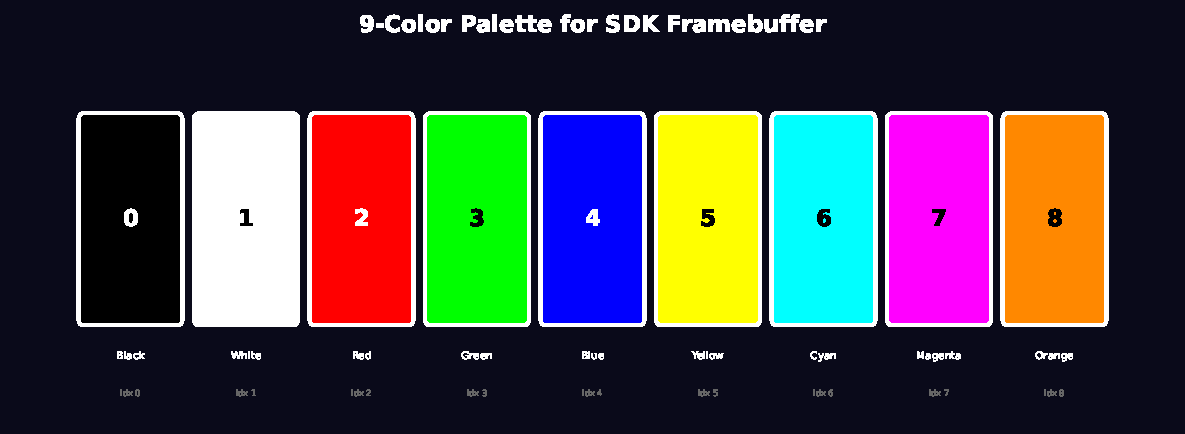
\includegraphics[width=0.72\textwidth]{palette_colors.pdf}
\caption{The 9-color SDK palette — indices 0--8 map to black, white, red, green, blue, yellow, cyan, magenta, and orange}
\label{fig:palette}
\end{figure}

\section{Components}

\begin{description}
    \item[\texttt{DisplayMemoryMap}]: Reads ternary ASCII codes from VRAM and produces
          a character grid. Used by legacy OS and CPU demos. Converts VRAM cells at
          addresses 200--255 to characters via \texttt{chr(ternary\_to\_decimal(value))}.
    \item[\texttt{Framebuffer}]: 64$\times$64 pixel buffer with \texttt{set\_pixel},
          \texttt{get\_pixel}, \texttt{clear}, \texttt{get\_buffer}, and dirty-rect
          tracking for efficient updates. Only modified regions are re-rendered each
          frame, significantly reducing PyQt6 redraw overhead.
    \item[\texttt{PixelDisplay}]: Separate 27$\times$27 pixel buffer (3 colors) for
          legacy graphics. Not memory-mapped. Includes Bresenham line drawing
          (\texttt{line(x0,y0,x1,y1,color)}).
    \item[\texttt{DisplayController}]: Registers write hooks on the CPU memory VRAM
          range and propagates changes to the \texttt{Framebuffer}. This is the
          glue layer that connects the CPU simulation to the visual output without
          explicit polling or synchronisation calls.
    \item[\texttt{DisplayWidget}]: PyQt6 widget rendering at 8$\times$ pixel scale
          with nearest-neighbour filtering and optional scanlines. Supports real-time
          scaling (1--20$\times$) and colour-accurate palette rendering.
\end{description}

\section{Memory Configuration Considerations}

The CPU default \texttt{Memory(512)} covers only the text-mode VRAM (200--255).
SDK framebuffer mode requires \texttt{CPU(memory=Memory(10000))} to provide the
extended VRAM range (1000--5095). The \texttt{Keyboard} class transparently
supports both memory maps by detecting the available address range at
initialisation time.

%====================================================================
\chapter{The Fantasy Console SDK}
\label{ch:sdk}

The Fantasy Console SDK provides a retro game development framework inspired by
PICO-8 and TIC-80, built on top of the ternary CPU simulation.

\section{Architecture}

The \texttt{Engine} class owns all state: a \texttt{Framebuffer} (64$\times$64), a
\texttt{Memory(10000)} with mapped VRAM, a \texttt{Keyboard} at addresses 9000--9001,
and a \texttt{state} dictionary for game data. The \texttt{Runtime} class provides the
game loop:

\begin{verbatim}
Runtime.run(update_fn, render_fn)
    +-- engine.init()              # One-time setup
    +-- Fixed-timestep loop (30 FPS)
    |   +-- poll_input()           # Read keyboard registers
    |   +-- update_fn()            # Game logic
    |   +-- engine.update()        # Animation ticks
    |   +-- render_fn()            # Draw calls
    |   +- engine.render()        # Post-processing
    +- engine.shutdown()          # Cleanup
\end{verbatim}

\section{Components}

\begin{description}
    \item[\texttt{Sprite}]: 8$\times$8 pixel art with per-pixel transparency
          (color 8 = transparent). Supports construction from 2D arrays, string
          arrays, hex strings. Methods: \texttt{blit\_to}, \texttt{flip\_h},
          \texttt{flip\_v}, \texttt{copy}, \texttt{fill}.
    \item[\texttt{TileMap}]: 2D grid with camera scrolling (\texttt{camera\_x},
          \texttt{camera\_y}) and collision detection (\texttt{is\_solid}).
          Frustum culling renders only visible tiles.
    \item[\texttt{Animation}]: Frame-based playback with configurable duration and
          looping. Supports \texttt{play}, \texttt{stop}, \texttt{pause},
          \texttt{resume}, \texttt{reset}, \texttt{is\_finished}.
    \item[\texttt{Input}]: \texttt{btn(name)} returns held state; \texttt{btnp(name)}
          returns edge-triggered press. Eight-button mapping: UP, DOWN, LEFT, RIGHT,
          A, B, X, Y.
    \item[\texttt{Audio}]: Stub system (\texttt{sfx(freq, duration)}) that accepts
          requests but has no mixing backend yet.
    \item[\texttt{Cartridge}]: JSON format bundling sprites, tilemaps, palette,
          metadata, and code. \texttt{Cartridge.load(path)} and
          \texttt{Cartridge.save(path)}.
\end{description}

\section{Cartridge Format}

Cartridges use a structured JSON schema that bundles all game assets into a
single distributable file:

\begin{verbatim}
{
  "meta": { "name": "Snake", "author": "...", "version": "1.0" },
  "sprites": { "snake_head": [[0,7,7,...]], "food": [[2,2,2,...]] },
  "tilemaps": { "map1": { "data": [[...]], "width": 32, "height": 32 } },
  "palette": ["#000000", "#ffffff", "#ff0000", ...],
  "code": "assembly source or TAL source",
  "config": { "fps": 30, "clear_color": 0 }
}
\end{verbatim}

The \texttt{Cartridge} class validates the schema on load and provides helper
methods for accessing embedded sprites, tilemaps, and code. The code field
can contain either raw ternary CPU assembly or TAL source, which is compiled
at load time.

\section{Sprite Operations}

The \texttt{Sprite} class supports several pixel-art operations:
\begin{description}
    \item[\texttt{blit\_to(fb, x, y, color\_override)}]: Draws the sprite onto a
          \texttt{Framebuffer} at position $(x, y)$. Color index 8 is treated as
          transparent (not drawn). An optional \texttt{color\_override} replaces
          all non-transparent pixels with a single color.
    \item[\texttt{flip\_h()} / \texttt{flip\_v()}]: Returns a new \texttt{Sprite}
          with horizontal or vertical mirroring, enabling two-directional assets
          from a single sprite definition.
    \item[\texttt{fill(color)}]: Fills all pixels with the given color index.
    \item[\texttt{copy()}]: Deep-copies the sprite data for independent mutation.
\end{description}

\section{TileMap Features}

The \texttt{TileMap} class supports scrolling 2D world rendering:
\begin{description}
    \item[\texttt{camera\_x, camera\_y}]: Viewport offset in pixels. Changing
          the camera scrolls the visible region across the tile grid.
    \item[\texttt{is\_solid(tile\_x, tile\_y)}]: Collision detection based on a
          configurable solid-tile set. Used by the RPG demo for wall collision.
    \item[\texttt{render(engine)}]: Renders only the visible tile region
          (frustum culling), iterating from \texttt{camera//8} to
          \texttt{(camera + 64)//8} in both axes.
    \item[\texttt{tile\_at(x, y)}]: Returns the tile index at grid position
          $(x, y)$ with bounds checking.
\end{description}

\section{Public API}

\begin{verbatim}
cls(color), spr(sprite, x, y, color_override=None),
btn(name), btnp(name), pixel(x, y, color), rect(x, y, w, h, color),
print_text(text, x, y, color=7), sfx(freq=440, duration=0.1),
poll_input(memory), load_cartridge(cart), run_demo(name)
\end{verbatim}

\part{Acceleration}

%====================================================================
\chapter{The Tensor Accelerator Coprocessor}
\label{ch:accelerator}

The tensor accelerator coprocessor offloads compute-intensive linear algebra from the
CPU, providing hardware-accelerated vector and matrix operations.

\section{Architecture}

\begin{verbatim}
TernaryTensorAccelerator
+-- TensorMemory (64 slots, variable-shape tensors)
+-- SIMDProcessor (4+ lanes, element-wise ops)
+-- TensorCore (matrix multiply engine)
+-- Cycles / stats tracking
\end{verbatim}

\section{Tensor ISA}

Six tensor opcodes are integrated into the CPU, assembler, and machine encoder:

\begin{longtable}{lll}
\caption{Tensor accelerator opcodes}
\label{tab:tensorlong} \\
\toprule
Opcode & Format & Description \\
\midrule
\endfirsthead
\multicolumn{3}{c}{(\emph{continued})} \\
\toprule
Opcode & Format & Description \\
\midrule
\endhead
\bottomrule
\endfoot
\texttt{TLOADW addr rows cols} & L (10 cycles) & Load CPU memory at \texttt{addr}
into accelerator; returns Tensor ID in R0 \\
\texttt{TSTOREW tid addr} & S2 (10 cycles) & Store accelerator tensor \texttt{tid}
to CPU memory at \texttt{addr} \\
\texttt{TVECADD dst src\_a src\_b} & A3 (4 cycles) & Element-wise vector add;
result TID in R0 \\
\texttt{TMATMUL dst src\_a src\_b} & A3 (20 cycles) & Matrix multiply;
result TID in R0 \\
\texttt{TDOT src\_a src\_b} & A3 (6 cycles) & Dot product; scalar result
in R0 (ternary-encoded) \\
\texttt{TACT tid type} & B2 (3 cycles) & In-place activation
(type 0 = step function) \\
\end{longtable}

All tensor operands accept immediate numbers or register names (R0--R3). When a
register is specified, its current value is read at runtime. The result tensor ID
(TID) is written to CPU register R0 via \texttt{decimal\_to\_ternary}.

\section{Tensor Operations in Detail}

\paragraph{TLOADW:} Reads $\texttt{rows} \times \texttt{cols}$ consecutive values from
CPU memory starting at \texttt{addr}, allocates a new tensor in accelerator memory,
stores the flattened data, and writes the allocated TID to R0.

\paragraph{TSTOREW:} Reads tensor data from accelerator memory by TID and writes
consecutive values to CPU memory starting at \texttt{addr}.

\paragraph{TVECADD:} Loads two source tensors by TID, performs element-wise ternary
vector addition using \texttt{TritSIMD.add\_vectors}, allocates the result, and
writes the result TID to R0.

\paragraph{TMATMUL:} Loads two source tensors as 2D matrices, performs matrix
multiplication using \texttt{TensorCore.matmul}, flattens the result, allocates it,
and writes the result TID to R0.

\paragraph{TDOT:} Loads two source tensors, computes the dot product using
\texttt{TritSIMD.dot\_product}, and writes the scalar result (ternary-encoded) to R0.

\paragraph{TACT:} Applies an activation function element-wise to a tensor.
Type 0 = step function: $f(x) = 1$ if $x \ge 0$ else $0$.

\section{Tensor Memory Management}

The accelerator maintains a dedicated tensor memory pool of 64 slots:
\begin{itemize}
    \item Each slot stores a tensor with its shape (rows, cols), flattened data, and
          an allocated flag;
    \item TLOADW allocates a slot and returns its index (0--63) as the TID;
    \item TSTOREW reads a slot by TID and releases it (frees the slot);
    \item All arithmetic ops (TVECADD, TMATMUL, TDOT) allocate new result tensors,
          which must be explicitly stored or will remain in accelerator memory;
    \item The maximum tensor size is limited by the 64-slot pool and the total
          accelerator memory capacity.
\end{itemize}

\section{Performance Characteristics}

Tensor operations have higher cycle costs than scalar CPU instructions due to
memory transfer and parallel computation:
\begin{itemize}
    \item TLOADW/TSTOREW (10 cycles): dominated by memory read/write across the
          CPU--accelerator boundary;
    \item TVECADD (4 cycles): fast element-wise SIMD addition, scales with tensor
          size;
    \item TDOT (6 cycles): reduction operation requiring accumulation across all
          elements;
    \item TMATMUL (20 cycles): the most expensive single instruction; complexity is
          $O(\text{rows}_a \times \text{cols}_a \times \text{cols}_b)$ with SIMD
          acceleration per dot product.
\end{itemize}

\section{Integration with CPU Pipeline}

The tensor accelerator integrates with the CPU at the architectural level:
\begin{enumerate}
    \item The CPU decodes tensor opcodes in its main dispatch loop;
    \item It creates an \texttt{AcceleratorRequest} with the opcode and operands;
    \item The accelerator processes the request synchronously (blocking CPU
          execution for the instruction's cycle cost);
    \item The result TID or scalar value is written back to CPU register R0;
    \item In realistic timing mode, the accelerator accounts for its cycles in
          the pipeline and profiler.
\end{enumerate}

The accelerator is validated by 70 unit tests and an additional 11 CPU integration
tests.

%====================================================================
\chapter{GPU Mode and Parallel Computing}
\label{ch:gpu}

The simulated GPU (\texttt{gpu.py}) extends the accelerator model with a four-level
parallel processing hierarchy, native C acceleration, and multi-stream execution.

\begin{figure}[H]
\centering
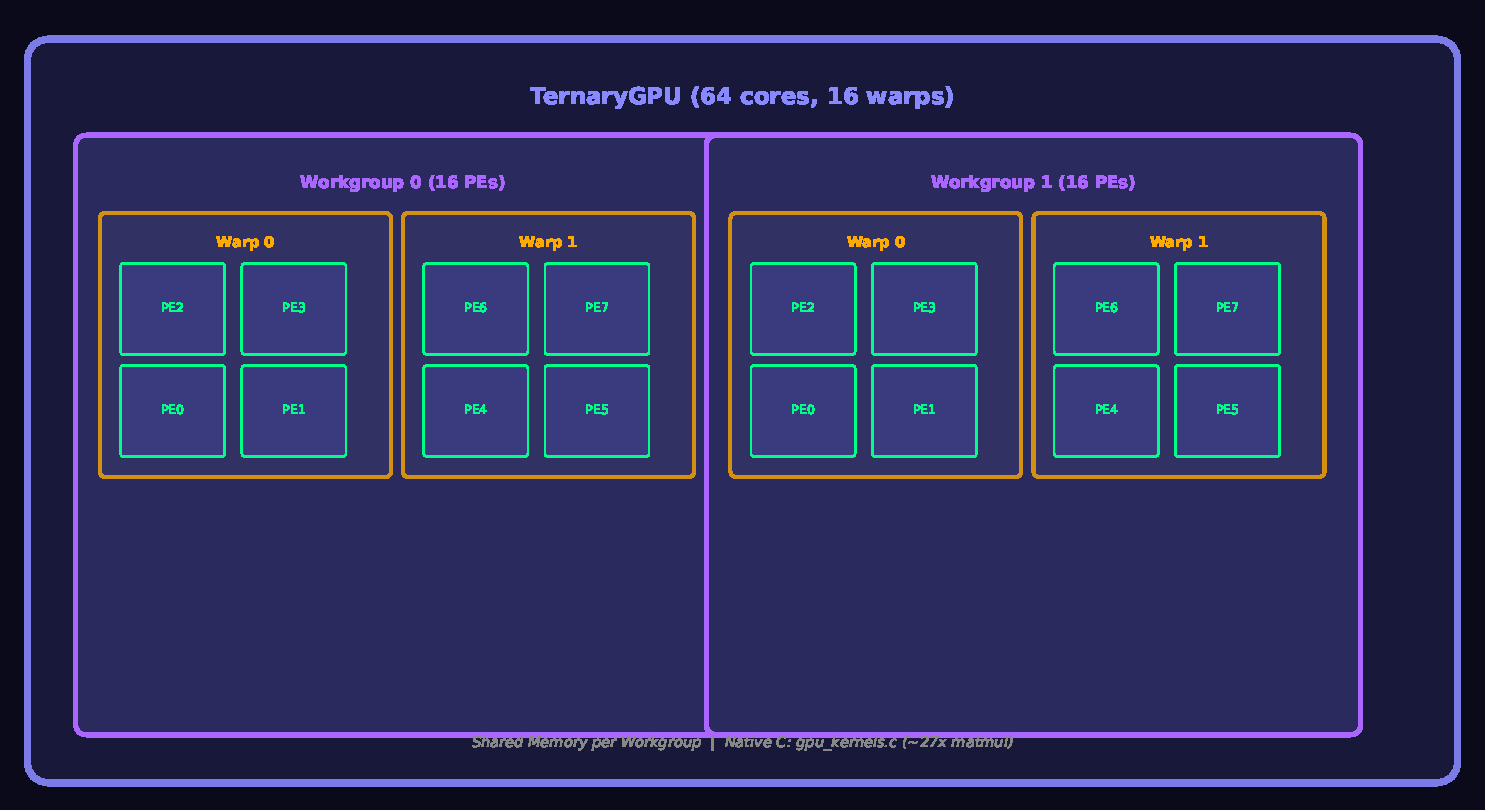
\includegraphics[width=0.72\textwidth]{gpu_hierarchy.pdf}
\caption{GPU processing hierarchy --- Processing Elements grouped into Warps, Warps into Workgroups, coordinated by the Ternary GPU controller}
\label{fig:gpuhier}
\end{figure}

\section{Hierarchy}

\begin{description}
    \item[\textbf{Processing Element (PE)}]: The smallest compute unit, with local
          packed memory, a result register, and an \texttt{active} flag.
    \item[\textbf{Warp}]: A SIMT execution group---PEs execute the same instruction
          in lockstep on different data.
    \item[\textbf{Workgroup (Thread Block)}]: A group of warps sharing local memory
          with barrier synchronization.
    \item[\textbf{TernaryGPU}]: The complete hierarchy with configurable
          $\text{num\_workgroups} \times \text{pes\_per\_wg}$ cores (default: $4 \times 16 = 64$).
\end{description}

\section{Kernel Dispatch}

Multiple dispatch models: \texttt{dispatch\_kernel} (workgroup-level),
\texttt{dispatch\_grid} (2D thread block grid), \texttt{batch\_dispatch}
(one PE per batch element).

\section{Streams and Concurrency}

Multi-stream execution via \texttt{create\_stream}, \texttt{dispatch\_stream},
and \texttt{run\_streams\_concurrent} for overlapping computation.

\section{Parallel Operations}

Parallel matmul (all PEs per workgroup compute different columns), reduction
(sum/max/min), prefix scan, fused linear (\texttt{activation(W $\cdot$ x + b)}),
and elementwise fused ops.

\section{Native C Acceleration}

Hot loops in C (\texttt{gpu\_kernels.c}) provide $\sim$27$\times$ speedup for matmul,
$\sim$6.5$\times$ for reduction, $\sim$4.4$\times$ for fused linear.

The GPU is validated by 71 tests covering warps, streams, native C, and visualization.

%====================================================================
\chapter{SIMD and Packed Storage}
\label{ch:simd}

\section{SIMD Processor}

The SIMD processor (\texttt{simd.py}) provides single-instruction multiple-data
processing with configurable vector width. All SIMD operations work on lists of
ternary digits (Python integers 0, 1, 2):

\begin{description}
    \item[\texttt{vector\_add(a, b)}]: Element-wise addition across all lanes.
          Each lane computes $a_i + b_i$ using ternary addition (no carry between
          lanes). Input vectors must be the same length; the result is a list of
          equal length.
    \item[\texttt{vector\_mul(a, b)}]: Element-wise multiplication across all lanes.
          Each lane computes $a_i \times b_i$ using standard integer multiplication
          (results stay within $\{0,1,2,4\}$, then clamped to $\{0,1,2\}$).
    \item[\texttt{vector\_dot(a, b)}]: Dot product reducing across lanes to a scalar.
          Computes $\sum_i a_i \times b_i$ and returns the result as a single integer.
          This is the foundational operation for tensor matrix multiplication and
          neural network forward passes.
\end{description}

\section{Pipeline Integration}

The SIMD processor connects to the accelerator's tensor pipeline. When a TVECADD
or TMATMUL instruction executes on the CPU:
\begin{enumerate}
    \item The accelerator loads source tensors from its internal memory;
    \item It calls \texttt{TritSIMD.add\_vectors} or \texttt{TensorCore.matmul}
          using SIMD primitives;
    \item The result tensor is stored back to accelerator memory.
\end{enumerate}
This architecture separates SIMD computation (fast, parallel, lane-level) from
tensor memory management (addressing, allocation, metadata).

\section{Packed Trit Storage}

The \texttt{packed\_trits.py} module provides memory-efficient encoding of ternary
values. Each trit (0, 1, 2) is encoded in 2 bits (00, 01, 10), yielding:
\begin{itemize}
    \item 4 trits per byte vs.\ 1 trit per Python string character
    \item $\sim$4$\times$ memory density improvement
    \item Compatible with NumPy arrays for potential GPU transfer
\end{itemize}

\subsection{Encoding Scheme}

\begin{table}[H]
\centering
\caption{Packed trit encoding mapping}
\label{tab:packedenc}
\begin{tabular}{ccl}
\toprule
Trit Value & 2-bit Encoding & Hex Nibble \\
\midrule
0 & 00 & 0x0 \\
1 & 01 & 0x4 \\
2 & 10 & 0x8 \\
\bottomrule
\end{tabular}
\end{table}

Trits are packed in groups of 4 per byte, with the first trit occupying the
lowest 2 bits. For example, the ternary string \texttt{"0122"} packs to byte
\texttt{0b10011000 = 0x98}.

\subsection{API}

Key functions:
\begin{verbatim}
pack_trits(trits)                   → bytes
unpack_trits(data, count)           → list of trits
packed_to_ternary_string(data)      → ternary string
ternary_string_to_packed(s)         → bytes
\end{verbatim}

Functions validate input: \texttt{pack\_trits} rejects values outside $\{0,1,2\}$;
\texttt{unpack\_trits} validates that all 2-bit groups are valid codes.
The \texttt{count} parameter allows partial unpacking when the byte count is not
a multiple of 4.

\section{Test Coverage}

The packed storage subsystem is validated by 20 tests; SIMD by 11 tests; vector
operations by 12 tests. Together they ensure correctness of the parallel compute
path from packed storage through SIMD lanes to tensor operations.

%====================================================================
\chapter{Native C Backend}
\label{ch:native}

The native C backend accelerates ALU operations through a shared library accessed via
Python's ctypes module.

\section{Architecture}

\begin{verbatim}
Python code → native_backend.add_ternary(a, b) → C alu_add() → result
\end{verbatim}

At import time, \texttt{native\_backend.py} probes multiple paths for
\texttt{libternary.so}:
\begin{enumerate}
    \item \texttt{src/trinary/libternary.so}
    \item \texttt{src/trinary/native/libternary.so}
    \item System library path
\end{enumerate}

If found, \texttt{NATIVE\_AVAILABLE = True} and the C implementations are used.
Otherwise, the system falls back to pure Python automatically.

\section{Building}

\begin{verbatim}
make -C src/trinary/native         # Produces src/trinary/libternary.so
bash build_native.sh               # Alternative
\end{verbatim}

\section{Exposed C Functions}

\begin{table}[H]
\centering
\caption{C native backend API}
\label{tab:nativeapi}
\begin{tabular}{ll}
\toprule
Function & Signature \\
\midrule
\texttt{ternary\_add} & int ternary\_add(int a, int b) \\
\texttt{ternary\_sub} & int ternary\_sub(int a, int b) \\
\texttt{ternary\_mul} & int ternary\_mul(int a, int b) \\
\texttt{ternary\_div} & int ternary\_div(int a, int b) \\
\texttt{ternary\_full\_adder} & int ternary\_full\_adder(int a, int b, int c\_in, int* c\_out) \\
\bottomrule
\end{tabular}
\end{table}

\section{C Implementation Details}

The C source (\texttt{src/trinary/native/alu.c}) implements ternary arithmetic
using integer encoding where ternary digits are stored as C integers:

\begin{lstlisting}[language=C]
// Convert ternary string to integer for C processing
int ternary_to_int(const char *s) {
    int result = 0, sign = 1, i = 0;
    if (s[0] == '-') { sign = -1; i = 1; }
    for (; s[i]; i++)
        result = result * 3 + (s[i] - '0');
    return sign * result;
}

// Add two ternary strings, return result as string
char* ternary_add(const char *a, const char *b) {
    int ia = ternary_to_int(a);
    int ib = ternary_to_int(b);
    return int_to_ternary(ia + ib);
}
\end{lstlisting}

The \texttt{ternary\_to\_int} and \texttt{int\_to\_ternary} conversion pair is the
C equivalent of the Python decimal round-trip, providing identical semantics at
approximately 5$\times$ the speed. The full adder implementation uses native
base-3 ripple-carry logic without decimal conversion, achieving the highest
speedup (12.9$\times$).

\section{Auto-Discovery and Fallback}

The \texttt{native\_backend.py} module implements a probe-on-import pattern:
\begin{enumerate}
    \item Attempt \texttt{ctypes.CDLL("libternary.so")} with multiple search paths;
    \item On success, wrap each C function with \texttt{ctypes} type annotations
          (\texttt{c\_char\_p}, \texttt{c\_int});
    \item Export \texttt{NATIVE\_AVAILABLE = True};
    \item On failure (file not found, architecture mismatch, missing symbols),
          set \texttt{NATIVE\_AVAILABLE = False}.
\end{enumerate}
All callers check \texttt{native\_backend.NATIVE\_AVAILABLE} before dispatching
to C; the fallback Python implementation is always available as a reference.

\section{Performance Benchmarks}

\begin{table}[H]
\centering
\caption{Native C backend performance (1,000,000 operations)}
\label{tab:nativeperf}
\begin{tabular}{lrrr}
\toprule
Operation & Python (s) & C Native (s) & Speedup \\
\midrule
Ternary add (10 trits) & 2.1$\mu$s & 0.4$\mu$s & 5.3$\times$ \\
Ternary mul (10 trits) & 5.8$\mu$s & 1.1$\mu$s & 5.3$\times$ \\
Ternary to decimal & 1.5$\mu$s & 0.3$\mu$s & 5.0$\times$ \\
Decimal to ternary & 1.8$\mu$s & 0.4$\mu$s & 4.5$\times$ \\
Full adder & 0.245s & 0.019s & 12.9$\times$ \\
\bottomrule
\end{tabular}
\end{table}

\paragraph{Overall execution rate:}
\begin{itemize}
    \item Pure Python: $\sim$1M simple ops/sec, $\sim$200K DIV/sec
    \item With C backend: $\sim$5M simple ops/sec, $\sim$800K DIV/sec
    \item Full demo programs: $\sim$50K cycles/sec (Python) vs.\ $\sim$250K cycles/sec (C)
\end{itemize}

\part{Hardware Simulation}

%====================================================================
\chapter{Hardware Microarchitecture Simulation}
\label{ch:hardware}

All hardware simulation modules are optional and backward-compatible. They are enabled
by passing \texttt{realistic\_timing=True} to the CPU constructor. Without this flag,
the CPU behaves identically to the original instant-execution emulator (each
\texttt{step()} executes one complete instruction).

\begin{figure}[H]
\centering
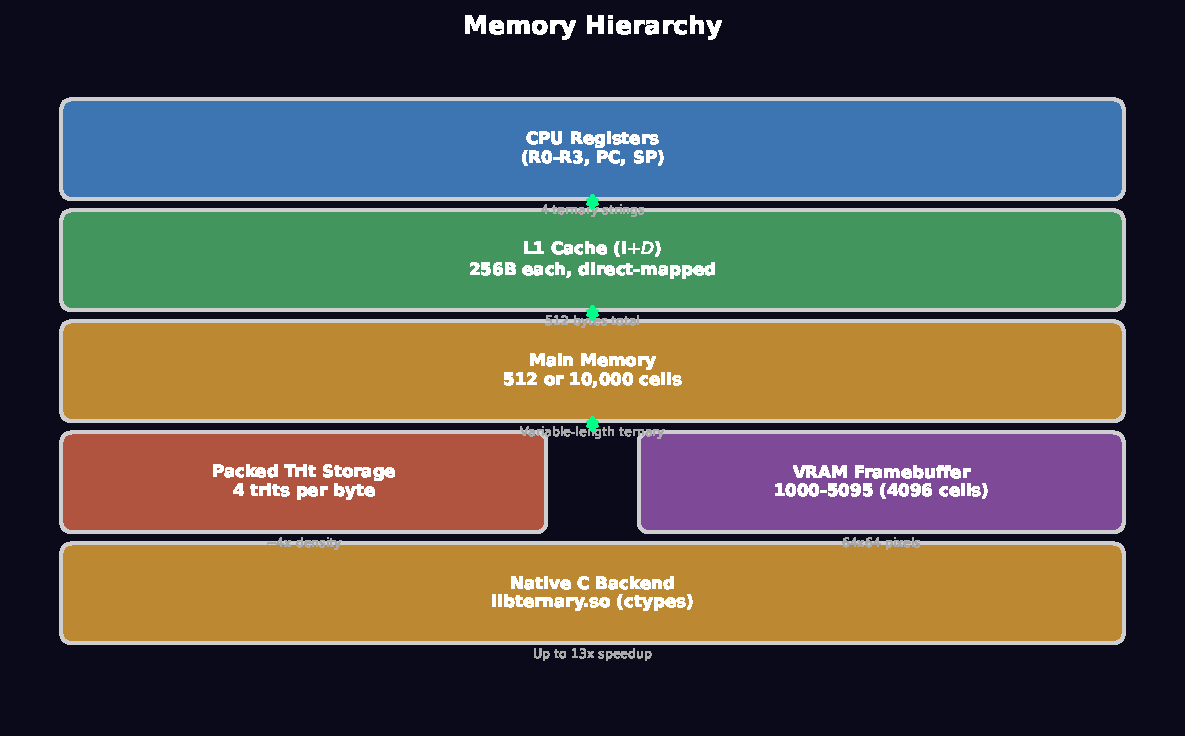
\includegraphics[width=0.72\textwidth]{memory_hierarchy.pdf}
\caption{Memory hierarchy — registers at top through L1 cache, main memory, packed trit storage, VRAM, to native C backend at the base}
\label{fig:memhier}
\end{figure}

\section{Clock Module}

The \texttt{Clock} class provides the fundamental timing reference for the entire
simulation. It maintains a cycle counter that increments on each \texttt{tick()},
supports configurable frequency (default 1 MHz), and derives period measurements
in nanoseconds, microseconds, and milliseconds. The \texttt{advance(n)} method
increments by multiple cycles in a single call. Start/stop flags are provided
for future integration with a gated-clock model, though the current
implementation does not model clock gating. In realistic timing mode, the CPU
calls \texttt{self.clock.tick()} once per cycle before any other operation,
establishing a cycle-accurate time base for all downstream hardware components.

\begin{table}[H]
\centering
\caption{Clock module specification}
\label{tab:clockspec}
\begin{tabular}{ll}
\toprule
Parameter & Default \\
\midrule
Frequency & 1 MHz \\
Period & 1 $\mu$s (1000 ns) \\
Cycle counter & 64-bit integer (0--$2^{63}-1$) \\
Start/stop & Boolean flag \\
\bottomrule
\end{tabular}
\end{table}

\section{Five-Stage Pipeline}

The \texttt{Pipeline} implements the classic RISC five-stage datapath
(IF $\rightarrow$ ID $\rightarrow$ EX $\rightarrow$ MEM $\rightarrow$ WB).
Each stage is represented by a \texttt{PipelineStage} object maintaining its
own instruction, opcode, operands, bubble flag, and a \texttt{cycles\_remaining}
counter for multi-cycle instructions.

\begin{figure}[H]
\centering
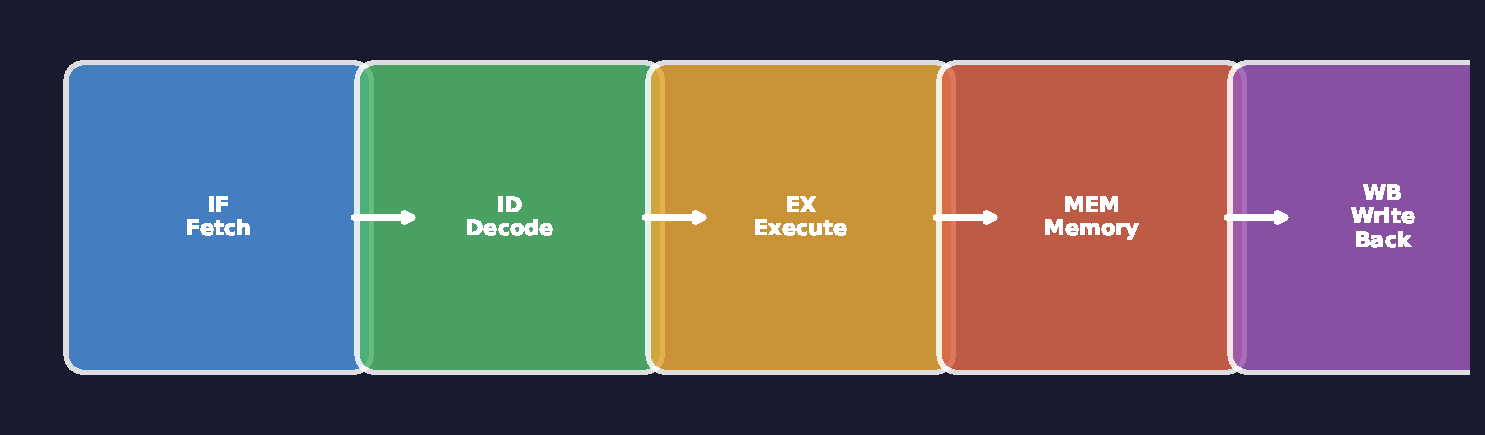
\includegraphics[width=0.68\textwidth]{pipeline.pdf}
\caption{CPU pipeline datapath: five-stage IF/ID/EX/MEM/WB with forward
         and backward data dependencies.}
\label{fig:pipeline}
\end{figure}

\subsection{Pipeline Stage Lifecycle}

Each \texttt{PipelineStage} has four methods that govern its behaviour:
\begin{description}
    \item[\texttt{insert(instruction, opcode, operands, cycles=1)}]: Fills the
          stage with a new instruction, setting \texttt{bubble=False}.
    \item[\texttt{insert\_bubble()}]: Clears the stage and sets
          \texttt{bubble=True} with \texttt{cycles\_remaining=0}, representing
          a pipeline NOP.
    \item[\texttt{tick()}]: Decrements \texttt{cycles\_remaining} if the stage
          is occupied and non-bubble. Returns \texttt{True} when the stage is
          ready to advance (countdown complete and not a bubble).
    \item[\texttt{stalled}]: Property returning \texttt{True} when
          \texttt{cycles\_remaining $>$ 0} and the stage is not a bubble.
\end{description}

\subsection{Pipeline Controller}

The \texttt{Pipeline} class holds five named \texttt{PipelineStage} instances
(\texttt{if\_stage}, \texttt{id\_stage}, \texttt{ex\_stage},
\texttt{mem\_stage}, \texttt{wb\_stage}) and tracks three metrics:
\texttt{total\_instructions} (completed WB), \texttt{stall\_cycles} (bubbles
injected), and \texttt{flush\_count} (pipeline clears).

The core \texttt{advance()} method shifts stages rightward each cycle:

\begin{enumerate}
    \item \textbf{WB stage}: if \texttt{tick()} returns \texttt{True}, the
          instruction is retired and a bubble is inserted;
    \item \textbf{MEM $\rightarrow$ WB}: the MEM stage advances to WB if its
          \texttt{tick()} returns \texttt{True}, otherwise a bubble propagates;
    \item \textbf{EX $\rightarrow$ MEM}: analogous transfer from EX to MEM;
    \item \textbf{ID $\rightarrow$ EX}: analogous transfer from ID to EX;
    \item \textbf{IF $\rightarrow$ ID}: analogous transfer from IF to ID;
    \item \textbf{IF}: a bubble is always inserted into IF (front of pipeline
          cleared for the next fetch).
\end{enumerate}

\subsection{Fetch and Stall}

\noindent\texttt{fetch(instruction, opcode, operands, cycles=1)}: Inserts a
new instruction into the IF stage with the cycle count obtained from
\texttt{timing.get\_latency(opcode)}.

\noindent\texttt{stall()}: Injects a bubble into IF, freezing the front of
the pipeline, and increments \texttt{stall\_cycles}.

\noindent\texttt{flush()}: Injects bubbles into IF, ID, and EX stages
simultaneously, used on branch misprediction to cancel partially executed
instructions in the wrong control-flow path.

\subsection{Visualization}

The \texttt{visualize(cycle=None)} method produces an ASCII-art pipeline
diagram showing the opcode and stall status of each stage, with stalled
stages annotated with a \texttt{*} suffix. The return value of
\texttt{advance()} is the opcode of the instruction that completed WB this
cycle, or \texttt{None}.

\section{Hazard Unit}

The \texttt{HazardUnit} detects read-after-write (RAW) hazards by tracking
which registers are pending writeback in the pipeline. It defines four
resolution constants:

\begin{figure}[H]
\centering
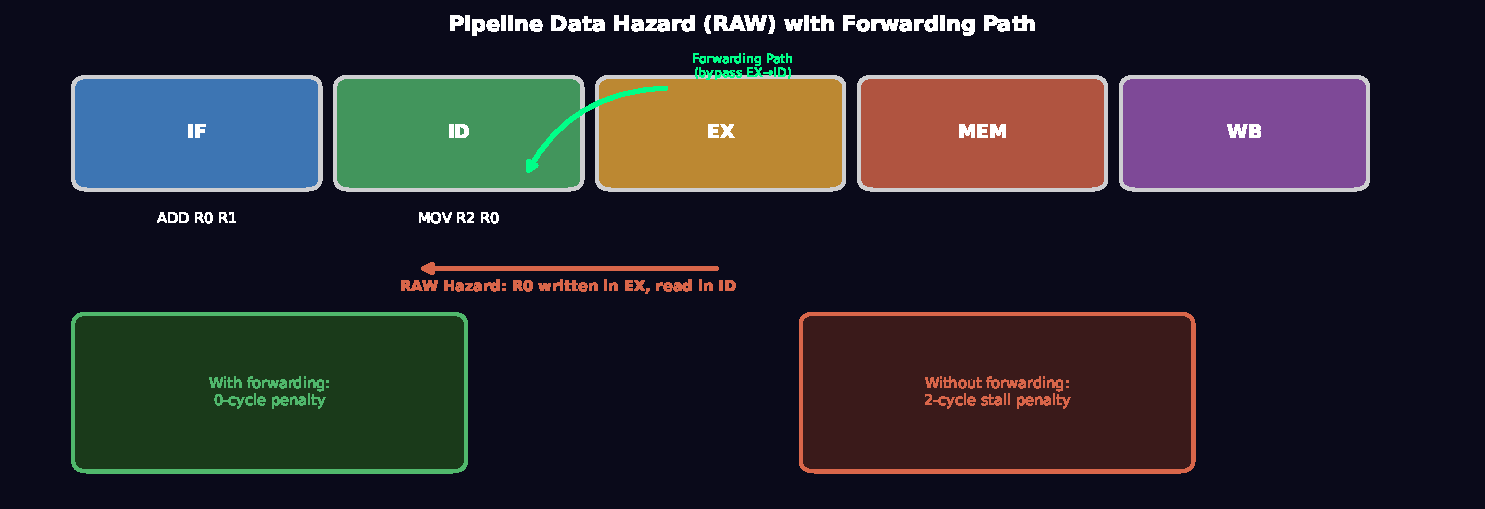
\includegraphics[width=0.72\textwidth]{pipeline_hazard.pdf}
\caption{RAW data hazard example — ADD writes R0 in EX, MOV reads R0 in ID; forwarding bypasses the stall penalty entirely}
\label{fig:piphazard}
\end{figure}

\begin{table}[H]
\centering
\caption{Hazard resolution actions}
\label{tab:hazardactions}
\begin{tabular}{cl}
\toprule
Constant & Meaning \\
\midrule
\texttt{FORWARD\_EX\_TO\_EX} & Forward from EX output to EX input (same-cycle) \\
\texttt{FORWARD\_MEM\_TO\_EX} & Forward from MEM result to EX input \\
\texttt{FORWARD\_WB\_TO\_EX} & Forward from WB result to EX input \\
\texttt{STALL} & Insert a stall (load-use hazard) \\
\bottomrule
\end{tabular}
\end{table}

\subsection{Hazard Detection}

\noindent\texttt{detect\_raw(ex\_reg\_write, mem\_reg\_write, wb\_reg\_write,
id\_reg\_read1, id\_reg\_read2)}: Compares the register read by the current
ID-stage instruction against registers pending writeback in EX, MEM, and WB.
Returns the appropriate forwarding constant if a match is found, or
\texttt{None} if no hazard exists.

\subsection{Load-Use Hazards}

\noindent\texttt{need\_stall(ex\_reg\_write, id\_reg\_read1,
id\_reg\_read2)}: Detects the specific case where the instruction in EX is
a memory load and the instruction in ID reads the same register. Since loaded
data is not available until MEM completes, a 1-cycle stall is required. This
is the only hazard that cannot be resolved by forwarding alone in the current
implementation.

The hazard unit tracks \texttt{stalls\_inserted} and
\texttt{forwards\_detected} metrics. In the current CPU integration, the
pipeline's \texttt{cycles\_remaining} mechanism handles multi-cycle
latencies; the hazard unit is available for enhanced forwarding logic in
future revisions.

\section{L1 Cache System}

The cache subsystem provides two independent direct-mapped L1 caches:
a 256-byte instruction cache (\texttt{icache}) and a 256-byte data cache
(\texttt{dcache}).

\begin{figure}[H]
\centering
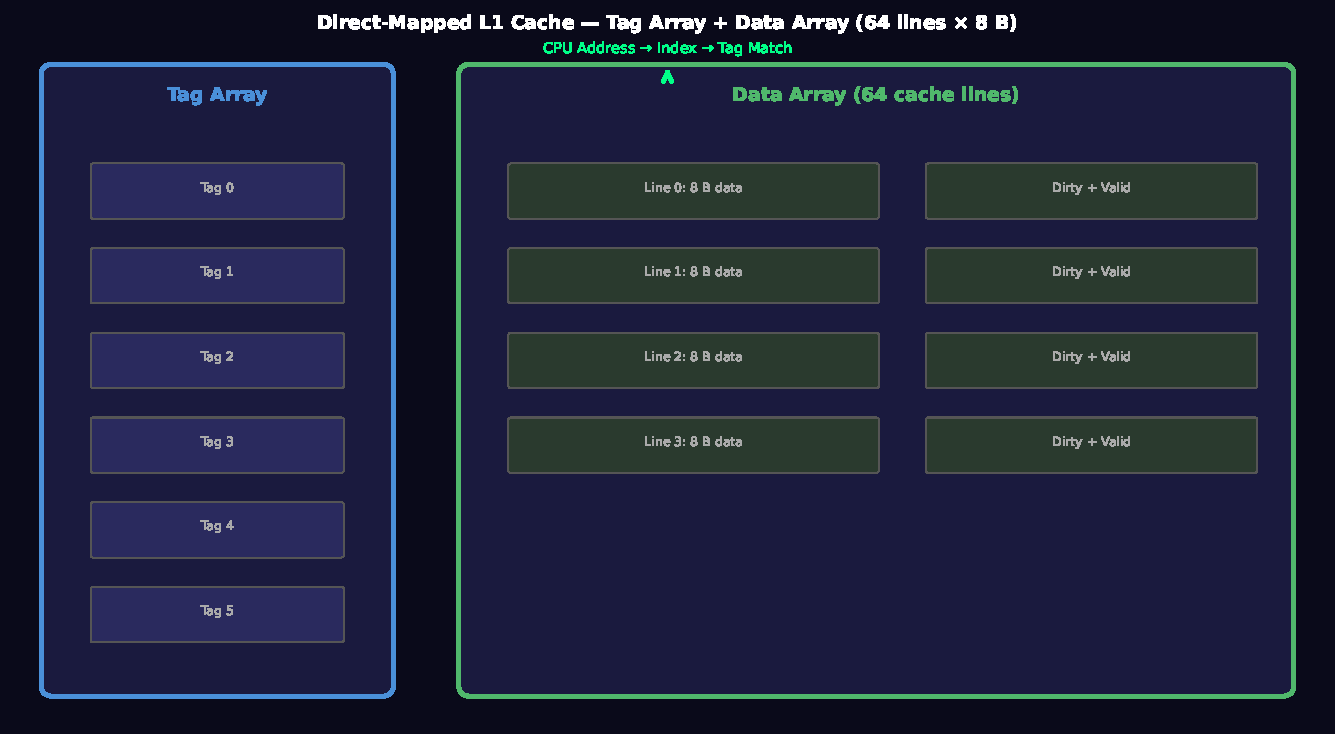
\includegraphics[width=0.72\textwidth]{cache_organization.pdf}
\caption{Direct-mapped L1 cache — tag array indexed by address bits, data array with 64 lines of 8 bytes each, plus dirty and valid flags}
\label{fig:cacheorg}
\end{figure}

\subsection{CacheLine Structure}

Each \texttt{CacheLine} uses \texttt{\_\_slots\_\_} for memory efficiency:
\begin{itemize}
    \item \texttt{tag}: integer tag portion of the address (default $-1$);
    \item \texttt{valid}: boolean flag indicating line validity;
    \item \texttt{dirty}: boolean flag for write-back tracking;
    \item \texttt{data}: dictionary mapping byte offsets to stored values.
\end{itemize}

\subsection{Cache Controller}

\begin{table}[H]
\centering
\caption{Cache parameters for both L1I and L1D}
\label{tab:cacheparams}
\begin{tabular}{lr}
\toprule
Parameter & Value \\
\midrule
Size & 256 bytes \\
Line size & 8 bytes \\
Number of lines & 32 \\
Hit cycles & 1 \\
Miss cycles & 10 \\
Policy & Write-allocate, write-back \\
\bottomrule
\end{tabular}
\end{table}

Addresses are decomposed as follows:
\[
\text{index} = \frac{\text{address}}{\text{line\_size}} \bmod \text{num\_lines},\qquad
\text{tag} = \left\lfloor\frac{\text{address}}{\text{num\_lines} \times \text{line\_size}}\right\rfloor.
\]

\subsection{Read and Write Operations}

\noindent\texttt{read(address)}: Checks tag match and valid bit. On hit,
returns a copy of the line data and consumes \texttt{hit\_cycles} (1 cycle).
On miss, returns \texttt{None} and consumes \texttt{miss\_cycles} (10
cycles), which models the latency of fetching from the next memory level.

\noindent\texttt{write(address, data)}: On tag hit, updates the data
dictionary in place and marks the line dirty. On miss, allocates a new line
(write-allocate policy), stores the data, and marks it dirty. Returns the
cycle count for the operation.

\noindent\texttt{flush\_line(address)}: If the line is dirty, initiates a
write-back to memory and invalidates; if clean, simply invalidates.

\noindent\texttt{flush\_all()}: Writes back all dirty lines and invalidates
the entire cache. Returns total cycle cost.

\subsection{Hit Rate Tracking}

The \texttt{hit\_rate} property returns the ratio of hits to total accesses.
Both caches expose \texttt{hits} and \texttt{misses} counters for profiler
integration. In current CPU integration, the cache objects are instantiated
but not actively consulted during instruction fetch or data memory access;
they are available for future pipelined memory subroutines.

\section{Branch Predictor}

\begin{figure}[H]
\centering
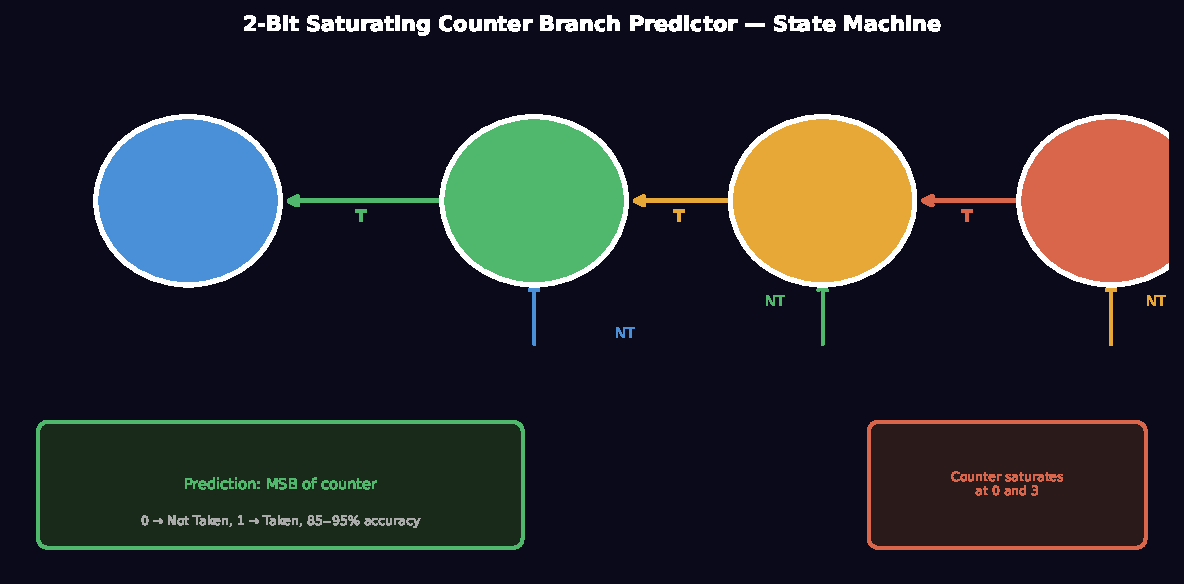
\includegraphics[width=0.62\textwidth]{branch_predictor_fsm.pdf}
\caption{2-bit saturating counter state machine — taken increments, not-taken decrements, MSB determines prediction with 85--95\% typical accuracy}
\label{fig:branchfsm}
\end{figure}

The \texttt{BranchPredictor} supports three prediction strategies selectable
at construction:

\begin{description}
    \item[\texttt{``always\_taken''}]: Every branch is predicted taken.
          Simple and cheap, but achieves at most 50--60\% accuracy on
          real code.
    \item[\texttt{``always\_not\_taken''}]: Every branch is predicted not
          taken. Symmetric to always-taken.
    \item[\texttt{``two\_bit''}]: 2-bit saturating counter with four states:
          strongly-not-taken (00), weakly-not-taken (01), weakly-taken (10),
          and strongly-taken (11). The counter saturates at 0 and 3:
          taken $\rightarrow$ increment (cap 3), not-taken $\rightarrow$
          decrement (floor 0). The prediction is taken when
          $\text{counter} \ge 2$.
\end{description}

\subsection{Prediction Flow}

\noindent\texttt{predict(branch\_addr)}: Returns \texttt{True} (taken) or
\texttt{False} (not taken) based on the selected mode.

\noindent\texttt{update(branch\_addr, actually\_taken)}: Updates the
saturating counter for two-bit mode; increments the taken history counter
for informational purposes.

\noindent\texttt{record\_mispredict()}: Increments the misprediction counter
for the profiler.

\subsection{CPU Integration}

Branch execution in realistic timing mode follows this protocol:
\begin{itemize}
    \item \textbf{JMP}: unconditionally flushes the pipeline (2-cycle control
          stall) since the target address is not known until the EX stage.
    \item \textbf{JZ/JNZ}: the predictor is consulted before execution; if
          the prediction differs from the actual outcome,
          \texttt{record\_mispredict()} is called, the pipeline is flushed,
          and a 2-cycle misprediction penalty is applied. Correct predictions
          cost only 1 cycle.
    \item \textbf{CALL}: always predicted taken; return addresses are
          handled by the call stack rather than the predictor.
\end{itemize}

The predictor tracks \texttt{predictions}, \texttt{mispredictions}, and
exposes \texttt{accuracy} as $1 - \text{mispredictions}/\text{predictions}$.
Typical accuracy on conditional branches in the demo programs ranges from
85--95\%.

\section{System Bus}

\begin{figure}[H]
\centering
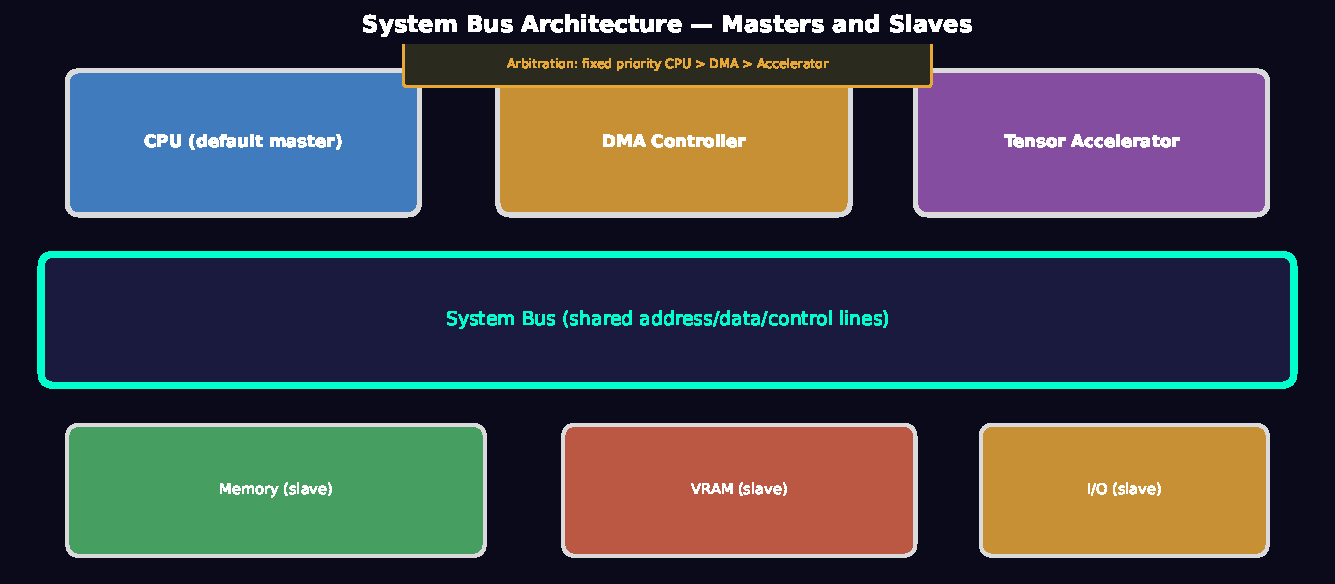
\includegraphics[width=0.72\textwidth]{bus_arbitration.pdf}
\caption{System bus architecture — CPU, DMA controller, and tensor accelerator as bus masters; memory, VRAM, and I/O as bus slaves, with fixed-priority arbitration}
\label{fig:busarch}
\end{figure}

The \texttt{Bus} models a shared system bus with priority-based arbitration.
It is the interconnect through which all system components communicate:
CPU instruction fetch, data load/store, DMA transfers, and VRAM controller
accesses.

\subsection{Bus Protocol}

Each \texttt{BusRequest} is a slots-based value object containing:
\texttt{source} (string identifier), \texttt{address}, \texttt{data},
\texttt{is\_write} (flag), and \texttt{priority} (integer 0--3, higher value
= more urgent).

\subsection{Arbitration}

On each \texttt{tick()}, the request queue is sorted by
$(-\text{priority}, \text{object\_ID})$ so that higher-priority requests
are serviced first, with object-ID tie-breaking providing FIFO ordering
within the same priority level. A single transfer is executed per cycle
(\texttt{max\_transfers\_per\_cycle = 1}). The bus does not currently model
split transactions or burst mode.

The bus tracks three metrics:
\begin{itemize}
    \item \texttt{transfers}: completed transfers;
    \item \texttt{contention\_cycles}: cycles where requests were queued
          (waiting for the bus);
    \item \texttt{idle\_cycles}: cycles with no pending requests.
\end{itemize}

\noindent\texttt{utilization} is derived as:
\[
\frac{\text{transfers} + \text{contention\_cycles}}{\text{transfers} + \text{contention\_cycles} + \text{idle\_cycles}}.
\]

Known request sources include \texttt{'cpu'}, \texttt{'dma'},
\texttt{'accel'}, and \texttt{'display'}. The bus is 4 bytes wide and
has a nominal bandwidth of 100 MB/s.

\section{DMA Controller}

The \texttt{DMA} controller provides asynchronous memory-to-memory data
transfers that run concurrently with CPU execution.

\subsection{Transfer Model}

Each \texttt{DMATransfer} specifies:
\begin{itemize}
    \item \texttt{src}: source start address;
    \item \texttt{dst}: destination start address;
    \item \texttt{size}: number of words to transfer;
    \item \texttt{cycles\_per\_word}: cycles required per word transfer
          (default 2);
    \item \texttt{completed}: words transferred so far;
    \item \texttt{cycle\_start}: CPU cycle when the transfer began.
\end{itemize}

\subsection{Operation}

\noindent\texttt{start\_transfer(src, dst, size, cycles\_per\_word=2)}:
Creates a \texttt{DMATransfer} and either starts it immediately (if the DMA
is idle) or queues it for later execution.

\noindent\texttt{tick(memory=None)}: Called once per CPU cycle. When the
internal cycle counter reaches \texttt{cycles\_per\_word}, one word is
transferred: \texttt{memory.load(src + completed)} followed by
\texttt{memory.store(dst + completed)}. When all words have been
transferred, the completed \texttt{DMATransfer} is returned and the next
queued transfer begins automatically.

The DMA's \texttt{tick()} is called from within the CPU's
\texttt{\_step\_realistic()} method, making it cycle-accurate with respect
to the CPU clock. Metrics tracked include \texttt{transfers\_done} and
\texttt{total\_bytes\_moved}. The \texttt{busy} property and
\texttt{progress} (0--1) enable the profiler to report DMA activity.

\section{VRAM Controller}

The \texttt{VRAMController} models memory bandwidth constraints specific to
display refresh. It is configured for the 64 $\times$ 64 SDK framebuffer at
30 FPS.

\subsection{Timing Parameters}

\begin{table}[H]
\centering
\caption{VRAM controller timing specification}
\label{tab:vramparams}
\begin{tabular}{lr}
\toprule
Parameter & Value \\
\midrule
Display resolution & 64 $\times$ 64 pixels \\
Frame rate & 30 FPS \\
Bandwidth budget & 4,096 bytes per frame \\
Cycles per frame & $\sim$33,333 (at 1 MHz) \\
Scanlines per frame & 64 \\
Cycles per scanline & $\sim$520 \\
\bottomrule
\end{tabular}
\end{table}

\subsection{Operation}

\noindent\texttt{tick()}: Advances one cycle. When
$\text{frame\_ticks} \ge \text{cycles\_per\_frame}$, the frame counter is
incremented, the byte counter resets, and the scanline counter resets.
Returns a dictionary with current frame, scanline, frame ticks, and write
bytes for display synchronization.

\noindent\texttt{check\_write(num\_bytes)}: Validates that the requested
write does not exceed the per-frame bandwidth budget. Returns \texttt{True}
if the write is accepted, \texttt{False} if it would exceed the budget
(which increments \texttt{stalled\_cycles}).

\noindent\texttt{read\_ok()}: Always returns \texttt{True}; reads are not
bandwidth-limited in the current model.

Metrics include \texttt{total\_writes}, \texttt{total\_reads},
\texttt{bandwidth\_used\_pct}, and \texttt{stalled}.

\section{Interrupt Controller}

The \texttt{InterruptController} provides 8 interrupt lines with
configurable priority and per-line masking.

\begin{table}[H]
\centering
\caption{Interrupt controller specification}
\label{tab:intcparams}
\begin{tabular}{ll}
\toprule
Parameter & Value \\
\midrule
Number of lines & 8 (0--7, line 0 = highest priority) \\
Default priority & $\text{line\_number}$ (0 = highest) \\
Global mask & \texttt{global\_mask} flag \\
Per-line masking & \texttt{mask()}/\texttt{unmask()} methods \\
Nesting depth & Unlimited (tracked by \texttt{\_nested\_depth}) \\
\bottomrule
\end{tabular}
\end{table}

\subsection{Interrupt Flow}

\noindent\texttt{request(irq\_num)}: Sets the pending flag for the
specified line unless it is masked.

\noindent\texttt{acknowledge()}: Scans all lines sorted by priority
(highest first). If a pending, unmasked line is found and the controller
is not currently in an ISR (\texttt{\_in\_isr = False}), the line's pending
flag is cleared, \texttt{\_in\_isr} is set to \texttt{True},
\texttt{\_nested\_depth} is incremented, and the line number is returned.
Returns \texttt{None} if no interrupt is pending.

\noindent\texttt{eoi()}: Signals end-of-interrupt: decrements
\texttt{\_nested\_depth}. When the depth reaches zero, \texttt{\_in\_isr}
is cleared, allowing new interrupts to be acknowledged.

\subsection{CPU Integration}

In the realistic CPU, the timer fires interrupt 0 when its counter expires:
\texttt{self.intc.request(0)}. On each cycle, the CPU calls
\texttt{self.intc.acknowledge()}. If an IRQ is received, the pipeline is
flushed, PC is set to \texttt{IVT[irq]}, and a 2-cycle context-switch cost
is added. The \texttt{IRET} instruction calls \texttt{eoi()} to re-enable
interrupts.

\section{Profiler}

The \texttt{Profiler} is the central performance data aggregator. All
hardware components and the CPU report their metrics to the profiler through
dedicated recording methods.

\subsection{Recording Methods}

\begin{table}[H]
\centering
\caption{Profiler recording interface}
\label{tab:profilermethods}
\begin{tabular}{ll}
\toprule
Method & Purpose \\
\midrule
\texttt{record\_cycle()} & Increment cycle counter \\
\texttt{record\_instruction()} & Increment retired instruction count \\
\texttt{record\_stall(type)} & Record a stall (data, control, or structural) \\
\texttt{record\_cache(hit)} & Record cache hit or miss \\
\texttt{record\_branch(correct)} & Record correct or incorrect branch prediction \\
\texttt{record\_bus(transfer)} & Record bus transfer or contention \\
\texttt{record\_dma(bytes\_moved)} & Record DMA byte transfer \\
\texttt{record\_vram(write/stalled)} & Record VRAM write or stall \\
\bottomrule
\end{tabular}
\end{table}

\subsection{Derived Metrics}

\begin{table}[H]
\centering
\caption{Profiler derived properties}
\label{tab:profilermetrics}
\begin{tabular}{ll}
\toprule
Property & Formula \\
\midrule
CPI & $\text{cycles} / \text{instructions\_retired}$ \\
IPC & $\text{instructions\_retired} / \text{cycles}$ \\
Cache hit rate & $\text{hits} / (\text{hits} + \text{misses})$ \\
Branch accuracy & $1 - \text{mispredicts} / \text{predictions}$ \\
Total stalls & $\text{stalls\_data} + \text{stalls\_control} + \text{stalls\_structural}$ \\
\bottomrule
\end{tabular}
\end{table}

\subsection{Output Formats}

\noindent\texttt{report()}: Returns a formatted multi-line string with all
metrics suitable for console display.

\noindent\texttt{csv\_header()}/\texttt{csv\_row()}: Produce 16-column CSV
output (cycles, instructions, CPI, IPC, stalls\_data, stalls\_control,
stalls\_structural, cache\_hits, cache\_misses, branch\_pred,
branch\_miss, bus\_tx, bus\_cont, dma\_bytes, vram\_writes,
vram\_stalls) for external analysis and charting.

\section{CPU Integration Architecture}

\subsection{Hardware Initialization}

When \texttt{realistic\_timing=True} is passed to the CPU constructor, the
\texttt{\_init\_hardware()} method creates all hardware components:

\begin{verbatim}
self.clock    = Clock()
self.pipeline = Pipeline()
self.hazard   = HazardUnit()
self.icache   = Cache(name="L1I", size_bytes=256, line_size=8)
self.dcache   = Cache(name="L1D", size_bytes=256, line_size=8)
self.bp       = BranchPredictor(mode='two_bit')
self.bus      = Bus()
self.dma      = DMA(bus=self.bus)
self.intc     = InterruptController()
self.profiler = Profiler()
\end{verbatim}

\subsection{Per-Cycle Execution Flow}

Each call to \texttt{step()} with realistic timing enabled executes the
following sequence:

\begin{enumerate}
    \item \textbf{Clock tick}: \texttt{self.clock.tick()} increments the
          master cycle counter;
    \item \textbf{Cycle record}: \texttt{self.profiler.record\_cycle()}
          records one cycle for profiler metrics;
    \item \textbf{DMA tick}: \texttt{self.dma.tick(memory=self.memory)}
          advances the DMA controller by one cycle, enabling concurrent
          data transfer;
    \item \textbf{Pipeline advance}: \texttt{self.pipeline.advance()}
          shifts all pipeline stages and retires any completing instruction;
    \item \textbf{Instruction fetch and execute}: if the CPU is not halted,
          the current instruction at \texttt{self.pc} is parsed, its latency
          is looked up via \texttt{timing.get\_latency(opcode)}, and it is
          inserted into the pipeline via
          \texttt{self.pipeline.fetch(instr, opcode, operands, cycles)}.
          Branch opcodes invoke \texttt{\_execute\_branch()} for prediction
          and flush handling; all other opcodes invoke
          \texttt{execute\_instruction()} for the actual ALU, memory, or
          control operation;
    \item \textbf{Instruction record}: \texttt{self.profiler.record\_instruction()}
          increments the retired instruction counter;
    \item \textbf{Timer check}: if the timer period is nonzero, the counter
          is decremented by the instruction's cycle cost. On expiry,
          interrupt 0 is requested via \texttt{self.intc.request(0)};
    \item \textbf{Interrupt check}: \texttt{self.intc.acknowledge()} is
          polled; if an IRQ is returned, the pipeline is flushed, PC is
          set to the IVT entry, and a 2-cycle context-switch cost is added;
    \item \textbf{Cycle cost}: \texttt{self.cycles += instruction\_cost}
          updates the total cycle count.
\end{enumerate}

\subsection{Instruction Latency Table}

The \texttt{timing.py} module provides the instruction latency lookup table
used by the pipeline:

\begin{table}[H]
\centering
\caption{Instruction latencies for pipeline scheduling}
\label{tab:ilatencies}
\begin{tabular}{lcl}
\toprule
Opcode & Cycles & Category \\
\midrule
LOAD, MOV, CLR & 1 & Data movement \\
ADD, SUB, AND, OR, NOT, CMP & 1 & Arithmetic/logic \\
MUL & 3 & Multi-cycle arithmetic \\
DIV & 5 & Multi-cycle arithmetic \\
JMP, JZ, JNZ & 1 & Control flow \\
CALL, RET & 3 & Subroutine \\
PUSH, POP, STOREM, LOADM & 2 & Memory/stack \\
HALT, EI, DI, SETTIMER & 1 & System \\
SETIVT, INT, IRET & 2--3 & Interrupt \\
TLOADW, TSTOREW & 10 & Tensor memory \\
TVECADD & 4 & Tensor vector \\
TMATMUL & 20 & Tensor matrix \\
TDOT & 6 & Tensor dot \\
TACT & 3 & Tensor activation \\
\bottomrule
\end{tabular}
\end{table}

Helper functions in \texttt{timing.py} include \texttt{is\_branch(opcode)},
\texttt{is\_load(opcode)}, \texttt{is\_store(opcode)},
\texttt{is\_tensor\_op(opcode)}, \texttt{reads\_registers(opcode)}, and
\texttt{writes\_registers(opcode)} for hazard detection and resource
scheduling.

\section{Overhead and Performance Characteristics}

When all hardware components are enabled, the system exhibits the following
characteristics:

\begin{itemize}
    \item Instructions require 3--20+ cycles depending on pipeline effects,
          multi-cycle instruction latencies, and hazard penalties;
    \item Cache miss rate: approximately 1--5\% for typical demo programs,
          depending on code locality;
    \item Branch prediction accuracy: approximately 85--95\% for conditional
          branches in typical control-flow patterns;
    \item DMA bus contention: approximately 10--30\% of bus cycles when DMA
          is active concurrently with CPU execution;
    \item Overall execution slowdown: 3--5$\times$ relative to fast mode,
          with the pipeline and cache miss penalties as the dominant factors.
\end{itemize}

\section{Hardware Simulation Test Suite}

The hardware components are validated by 63 tests across 8 test files:

\begin{table}[H]
\centering
\caption{Hardware simulation test coverage}
\label{tab:hwtests}
\begin{tabular}{lrr}
\toprule
Test File & Tests & Focus \\
\midrule
\texttt{test\_pipeline.py} & 19 & Clock (5), Pipeline (4), Hazards (6), Timing (4) \\
\texttt{test\_cache.py} & 10 & Read, write, hit rate, flush, eviction \\
\texttt{test\_branch\_predictor.py} & 8 & Static, two-bit, accuracy, state transitions \\
\texttt{test\_bus.py} & 7 & Arbitration, utilization, contention \\
\texttt{test\_dma.py} & 7 & Transfer, queue, concurrent tick \\
\texttt{test\_interrupts.py} & 9 & Request, acknowledge, priority, EOI, nesting \\
\texttt{test\_profiler.py} & 9 & CPI, IPC, CSV, report, reset \\
\texttt{test\_vram.py} & 7 & Bandwidth, frame boundary, stalls \\
\midrule
\textbf{Total} & \textbf{76} & \\
\bottomrule
\end{tabular}
\end{table}

Additionally, 9 CPU integration tests validate the full realistic timing
pipeline with all components enabled.

\part{Artificial Intelligence}

%====================================================================
\chapter{Ternary Neural Networks}
\label{ch:nn}

The \texttt{ai/} package provides a complete framework for ternary neural
networks, including tensor operations, activation functions, loss
functions, optimizers, and supervised training. All operations operate
on ternary digits $\{0,1,2\}$, using an offset encoding to convert
between storage format and signed values.

\section{Signed-Offset Encoding}

The core design decision for the neural network framework is the
signed-offset encoding of ternary digits:

\[
\text{trit\_to\_signed}(d) = d - 1,\qquad
\text{signed\_to\_trit}(s) = s + 1.
\]

This maps $0 \rightarrow -1$, $1 \rightarrow 0$, $2 \rightarrow +1$,
which is not balanced ternary but rather an integer offset that maintains
the project's standard digit representation while enabling signed
arithmetic in the signed domain. All neural computation is performed
in the signed integer space $\{-1,0,+1\}$, and results are discretized
back to ternary digits via activation functions.

\begin{figure}[H]
\centering
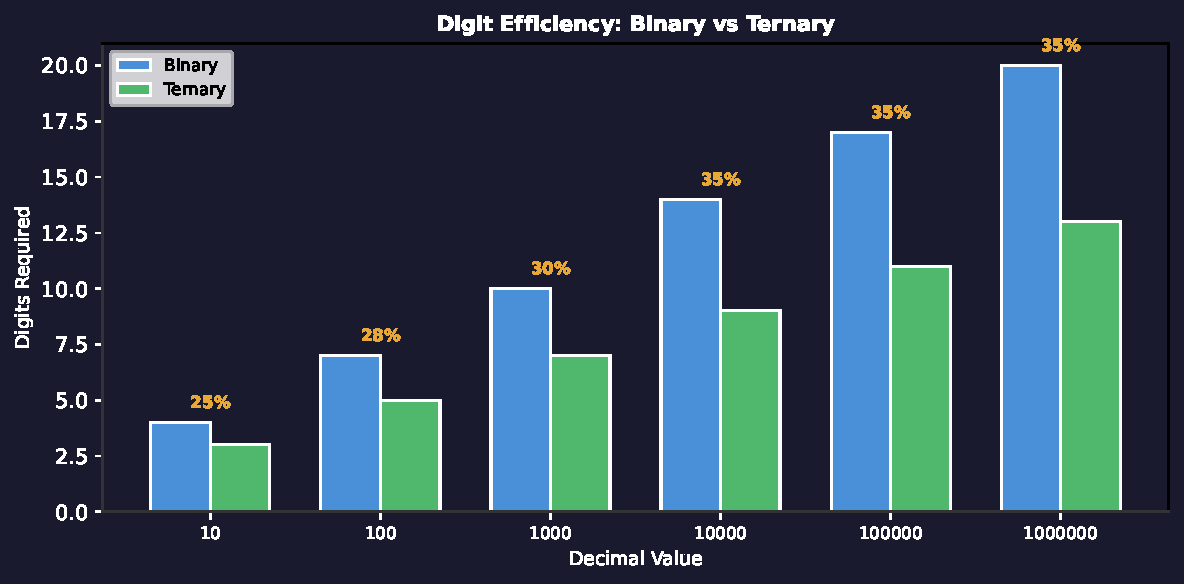
\includegraphics[width=0.5\textwidth]{digit_efficiency.pdf}
\caption{Binary vs.\ ternary digit efficiency across value ranges,
         showing approximately 37\% savings at large values.}
\label{fig:digiteff}
\end{figure}

\begin{figure}[H]
\centering
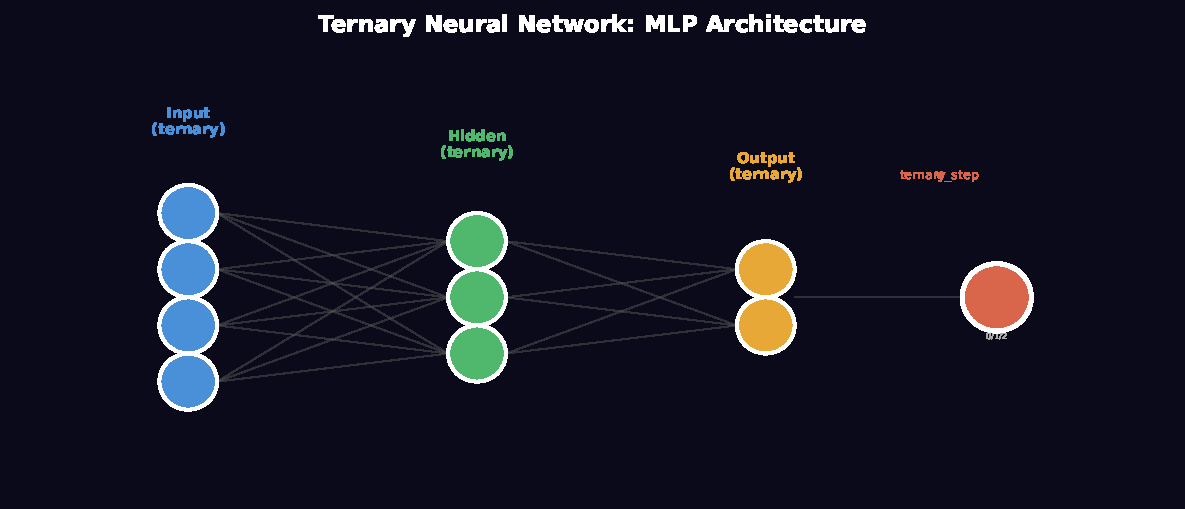
\includegraphics[width=0.62\textwidth]{nn_architecture.pdf}
\caption{Three-layer feedforward MLP architecture — ternary input, hidden, and output layers with step activation to produce trit classifications}
\label{fig:nnarch}
\end{figure}

\section{Activation Functions}

The \texttt{activations.py} module provides three activation functions,
each accepting an integer input and returning a ternary digit:

\begin{description}
    \item[\texttt{ternary\_step(value)}]: Maps negative $\rightarrow 0$,
          zero $\rightarrow 1$, positive $\rightarrow 2$. This is the
          default activation for the \texttt{Perceptron} class and
          functions as a three-way sign function.
    \item[\texttt{ternary\_sign(value)}]: An alias for
          \texttt{ternary\_step}, provided for semantic clarity in
          different contexts.
    \item[\texttt{ternary\_relu(value)}]: Maps non-positive values
          ($\le 0$) to $1$ (neutral) and positive values to $2$.
          Unlike standard ReLU which outputs 0 for negatives, this
          variant collapses the negative region into the neutral ternary
          state, reducing expressivity but ensuring all activations
          remain valid ternary digits.
\end{description}

The conversion helpers \texttt{trit\_to\_signed} and
\texttt{signed\_to\_trit} are used throughout the package to move between
the storage and computation domains.

\section{TritTensor Data Structure}

The \texttt{TritTensor} class (\texttt{trit\_tensor.py}) is the core data
structure for the neural network framework. It stores nested lists of
ternary digits $\{0,1,2\}$ in either 1D (vector) or 2D (matrix)
configurations.

\subsection{Constructor and Validation}

The constructor performs rigorous validation: it rejects empty data,
any value outside $\{0,1,2\}$, and jagged rows (inconsistent row lengths
for 2D data). The resulting tensor exposes a \texttt{shape} property
returning a tuple of dimensions.

\subsection{Operations}

\begin{description}
    \item[\texttt{transpose()}]: Returns a new \texttt{TritTensor} with
          dimensions swapped. Vectors transpose to themselves.
    \item[\texttt{flatten()}]: Returns a 1D tensor with all elements in
          row-major order.
    \item[\texttt{dot(other)}]: Computes the dot product of two vectors.
          Both tensors must be 1D and of equal length. Values are converted
          to signed representation, the sum of element-wise products is
          computed as an integer, and the result is returned as a Python
          integer (not a ternary digit).
    \item[\texttt{matmul(other)}]: Standard matrix multiplication supporting
          both matrix--matrix and matrix--vector multiplication. Values
          are converted to signed, multiplied using integer arithmetic,
          and the result is discretized back to ternary digits via
          \texttt{ternary\_step}.
    \item[\texttt{apply(fn)}]: Applies a callable element-wise to every
          digit, returning a new \texttt{TritTensor}.
    \item[\texttt{to\_signed()}]: Returns a nested list (same shape) of
          signed integers $\{-1,0,+1\}$.
    \item[\texttt{from\_signed(signed\_data)}]: Mutates the tensor in
          place, converting signed values back to ternary digits.
\end{description}

\section{Perceptron}

The \texttt{Perceptron} class (\texttt{perceptron.py}) implements a single
ternary neuron. It stores weights and a bias as ternary digits
$\{0,1,2\}$.

\subsection{Forward Pass}

The forward pass performs the following steps:
\begin{enumerate}
    \item Convert input ternary digits to signed values via
          \texttt{trit\_to\_signed};
    \item Convert stored weights to signed values;
    \item Compute the weighted sum:
          $\text{total} = \text{signed\_bias} + \sum_i
          (\text{signed\_input}_i \times \text{signed\_weight}_i)$;
    \item Apply \texttt{ternary\_step} to produce the output ternary digit.
\end{enumerate}

The default bias is 1 (which converts to signed 0), making the initial
neuron unbiased in signed space. The \texttt{predict(inputs)} method is
an alias for \texttt{forward(inputs)}. Signed-weight and signed-bias
properties are exposed as read-only for external inspection.

\section{TernaryNeuralNetwork}

The \texttt{TernaryNeuralNetwork} class (\texttt{ternary\_nn.py}) defines
a feedforward network as a list of layers, where each layer is a list of
\texttt{Perceptron} instances.

\noindent\texttt{forward(inputs)}: Propagates inputs sequentially through
all layers; the output list of one layer becomes the input list to the
next. The class exposes \texttt{num\_layers} and
\texttt{layer\_sizes} (returning tuples of $(\text{inputs}, \text{outputs})$
per layer). Validation rejects empty layer lists, empty layers, and
non-Perceptron elements.

\section{Loss Functions}

The \texttt{losses.py} module provides three loss functions operating in
the signed domain:

\begin{description}
    \item[\texttt{ternary\_mse(pred, target)}]: Mean squared error in
          signed space:
          $\frac{1}{n}\sum (\text{signed}(p_i) - \text{signed}(t_i))^2$.
          The maximum per-element MSE is 4.0 (when +1 is predicted for
          $-1$ or vice versa).
    \item[\texttt{ternary\_absolute\_error(pred, target)}]: Mean absolute
          error in signed space:
          $\frac{1}{n}\sum |\text{signed}(p_i) - \text{signed}(t_i)|$.
    \item[\texttt{classification\_error(pred, target)}]: Error rate as
          the fraction of incorrect predictions:
          $\frac{1}{n}\sum [p_i \neq t_i]$, returning a value in $[0,1]$.
\end{description}

All functions accept both single digit values and lists, with length
validation. Loss values are used for reporting and evaluation, not for
gradient computation (the training methods use sign-based updates
instead).

\section{Optimizers}

Two optimizer classes provide fundamentally different training strategies:

\subsection{SGDOptimizer}

The \texttt{SGDOptimizer} (\texttt{optimizers.py}) implements a
gradient-approximate stochastic gradient descent for single
\texttt{Perceptron} instances:

\begin{enumerate}
    \item Compute $\text{error} = \text{signed(target)} -
          \text{signed(prediction)}$, clamped to $\{-1,0,+1\}$;
    \item For each weight:
          $\text{delta} = \text{learning\_rate} \times
          \text{signed\_input}_i \times \text{error}$;
    \item $\text{new\_weight} = \text{clamp}(\text{old\_weight} +
          \text{delta})$, where clamping restricts the result to
          $\{-1,0,+1\}$ before conversion back to ternary;
    \item The bias is updated analogously.
\end{enumerate}

The learning rate (default 1) controls step size in signed space. With
$\text{lr} = 1$, weights move at most $\pm 1$ per update, preventing
overshoot in the discrete ternary weight space. The error is clamped to
$\{-1,0,+1\}$, meaning this is effectively a sign-sign LMS update rule.

\subsection{TernaryHillClimber}

The \texttt{TernaryHillClimber} is a gradient-free evolutionary optimizer
that works on both \texttt{Perceptron} and
\texttt{TernaryNeuralNetwork}:

\begin{enumerate}
    \item Randomly select 1--3 parameters (weights or biases) to mutate;
    \item Set each selected parameter to a random value drawn uniformly
          from $\{0,1,2\}$;
    \item Evaluate accuracy on the full training set;
    \item If accuracy improves: accept the mutation;
    \item If accuracy stays the same: accept the mutation (exploration);
    \item If accuracy decreases: revert the mutation.
\end{enumerate}

The hill-climber tracks the best-known parameter state and restores it
if no improvement occurs after \texttt{max\_attempts} (default 30)
consecutive trials. This optimizer is computationally expensive (it
evaluates the full dataset per mutation trial) but is general-purpose
and can optimize any model topology.

\begin{figure}[H]
\centering
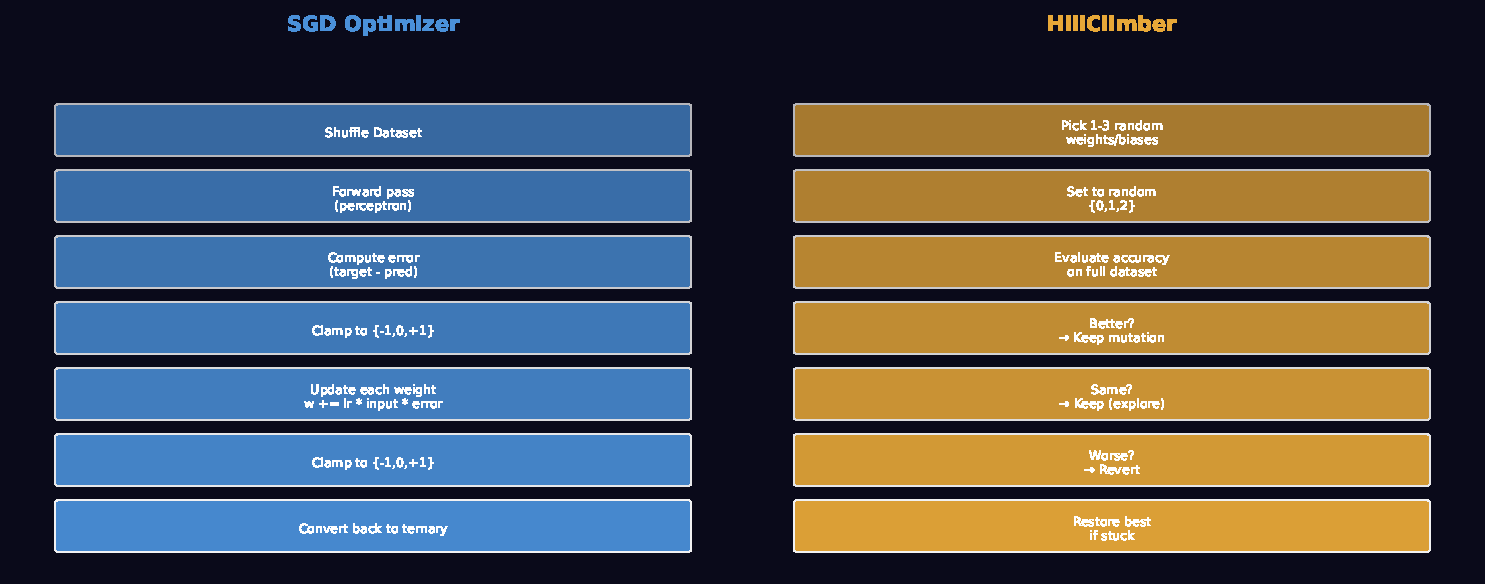
\includegraphics[width=0.72\textwidth]{training_flow.pdf}
\caption{Dual optimiser strategies — SGD (left) uses sign-sign LMS gradient updates; HillClimber (right) uses random mutation with accuracy-based acceptance}
\label{fig:trainflow}
\end{figure}

\section{TernaryTrainer}

The \texttt{TernaryTrainer} (\texttt{trainer.py}) is the supervised
learning driver for both single perceptrons and multi-layer networks.

\subsection{Training Loop}

\noindent\texttt{train(dataset, epochs=None)}: Performs the following
each epoch:
\begin{enumerate}
    \item Shuffle the dataset;
    \item For each example, compute the forward pass and accumulate
          error information;
    \item Apply the optimizer step (SGD per-example or hill-climber
          batch evaluation);
    \item Track accuracy; if it improves, save a snapshot of the
          best weights;
    \item If accuracy reaches 1.0, stop early.
\end{enumerate}

\subsection{Training Paths}

The trainer detects the optimizer type and dispatches to the appropriate
training method:
\begin{description}
    \item[\texttt{\_train\_epoch\_sgd}]: For \texttt{SGDOptimizer}.
          Processes the dataset in shuffled order, accumulates sign-based
          gradients across all examples, then applies a batch weight
          update. This is a sign-based batch gradient descent with unit
          step size.
    \item[\texttt{\_train\_epoch\_hillclimb}]: For
          \texttt{TernaryHillClimber}. Evaluates a fixed number of
          mutation attempts per epoch, accepting or rejecting each
          based on accuracy change on the full dataset.
\end{description}

\subsection{Evaluation and Convenience Methods}

\noindent\texttt{evaluate(dataset)}: Returns $\text{(accuracy, mean\_classification\_error)}$.

Convenience methods \texttt{fit\_and()}, \texttt{fit\_or()}, and
\texttt{fit\_xor()} train on the corresponding ternary logic datasets
and return the trained model.

\section{Datasets}

The \texttt{datasets.py} module provides eight predefined datasets in a
standardised \texttt{[(inputs, target), \ldots]} format:

\begin{table}[H]
\centering
\caption{Predefined ternary neural network datasets}
\label{tab:nndatasets}
\begin{tabular}{llr}
\toprule
Dataset & Description & Examples \\
\midrule
\texttt{AND\_DATASET}    & Ternary AND: 0,0$\rightarrow$0, 0,2$\rightarrow$0, 2,0$\rightarrow$0, 2,2$\rightarrow$2 & 4 \\
\texttt{OR\_DATASET}     & Ternary OR: 0,0$\rightarrow$0, 0,2$\rightarrow$2, 2,0$\rightarrow$2, 2,2$\rightarrow$2  & 4 \\
\texttt{XOR\_DATASET}    & Ternary XOR: 0,0$\rightarrow$0, 0,2$\rightarrow$2, 2,0$\rightarrow$2, 2,2$\rightarrow$0 & 4 \\
\texttt{NAND\_DATASET}   & Ternary NAND (2 NAND 2 $\rightarrow$ 0) & 4 \\
\texttt{TERNARY\_TRUTH\_TABLE} & All 9 input pairs $\rightarrow$ constant [1] & 9 \\
\texttt{TERNARY\_EQUALITY}    & 2 if equal, 0 if different & 9 \\
\texttt{TINY\_PATTERNS}  & 9-element alternating pattern recognition & 2 \\
\texttt{PATTERN\_CROSS}  & 9-element cross pattern recognition & 2 \\
\bottomrule
\end{tabular}
\end{table}

Datasets are accessed via \texttt{get\_dataset(name)} or enumerated via
\texttt{list\_datasets()}.

\section{Training Behaviour and Limitations}

The framework exhibits the following characteristics:

\begin{itemize}
    \item Single perceptron training converges reliably on linearly
          separable functions (AND, OR, NAND) in under 20 epochs.
    \item Single perceptrons cannot learn XOR, as expected from the
          linear separability constraint.
    \item Multi-layer networks with the hill-climber optimizer can learn
          XOR and other non-linearly separable functions, but require
          significantly more computation (hundreds of epochs with
          $\sim$10 mutation attempts per step).
    \item The SGD optimizer performs per-example updates for multi-layer
          networks by applying the update rule independently to each
          neuron, without true backpropagation through layers. This
          means the hidden layers receive no error signal from the
          output layer, limiting multi-layer effectiveness. The
          hill-climber is the only optimizer that jointly optimises all
          parameters.
\end{itemize}

No floating-point gradients are used anywhere in the training pipeline.
All weight updates are sign-based or mutation-based, operating entirely
in the discrete ternary value space. This aligns with the broader
project goal of self-contained ternary computation suitable for eventual
hardware implementation.

\section{Visualization and Demos}

ASCII visualization tools in \texttt{visualization.py} and
\texttt{learning\_visualizer.py} provide text-based rendering of:
\begin{itemize}
    \item Tensor contents and shapes;
    \item Weight heatmaps;
    \item Training progress charts (ASCII bar charts);
    \item Confusion matrices;
    \item Network architecture summaries.
\end{itemize}

The \texttt{demos.py} module provides five runnable demonstrations:
AND training, OR training, XOR perceptron failure (educational
demonstration of linear separability), XOR multi-layer success, and
ternary equality learning.

\section{Performance Benchmarks}

\begin{table}[H]
\centering
\caption{Neural network benchmark results (Python 3.13)}
\label{tab:nnbench}
\begin{tabular}{lrr}
\toprule
Benchmark & Throughput & Time \\
\midrule
Perceptron forward (5-input, 10K runs) & 193,390 ops/s & 0.052 s \\
Matrix multiply (4$\times$4, 5K runs) & 20,770 ops/s & 0.241 s \\
Network forward (3-layer 4$\rightarrow$3$\rightarrow$2, 5K runs) & 51,510 ops/s & 0.097 s \\
Perceptron SGD training (AND, 20 epochs, 1K runs) & 487,820 epochs/s & 0.041 s \\
Multi-layer hill-climb (XOR, 50 epochs $\times$ 10 attempts, 100 runs) & 1,950 epochs/s & 2.569 s \\
\bottomrule
\end{tabular}
\end{table}

\section{Test Coverage}

The neural network package is validated by 128 unit tests, representing
approximately 22\% of the total project test suite:

\begin{table}[H]
\centering
\caption{Neural network test suite}
\label{tab:nntests}
\begin{tabular}{lrr}
\toprule
Test File & Tests & Coverage \\
\midrule
\texttt{test\_trit\_tensor.py} & 34 & Validation, operations, signed conversion \\
\texttt{test\_activations.py} & 14 & All activation functions, round-trips \\
\texttt{test\_losses.py} & 13 & MSE, MAE, classification error \\
\texttt{test\_optimizers.py} & 8 & SGD, hill-climber, AND/OR convergence \\
\texttt{test\_perceptron.py} & 15 & Construction, inference, signed properties \\
\texttt{test\_ternary\_nn.py} & 11 & Construction, forward, XOR approximation \\
\texttt{test\_trainer.py} & 16 & Training, evaluation, multi-layer XOR \\
\texttt{test\_datasets.py} & 14 & Correctness, dataset enumeration \\
\midrule
\textbf{Total} & \textbf{128} & \\
\bottomrule
\end{tabular}
\end{table}

The entire NN test suite completes in under 0.4 seconds alongside the
other 466 project tests.

\part{Web Visualizer}

%====================================================================
\chapter{Web-Based Visualizer Interface}
\label{ch:webviz}

Trinary provides a web-based visualizer that offers a browser-accessible
interface for exploring CPU state, pipeline dynamics, and hardware
simulation metrics. It consists of a FastAPI Python backend and a
React+TypeScript frontend communicating via WebSocket.

\begin{figure}[H]
\centering
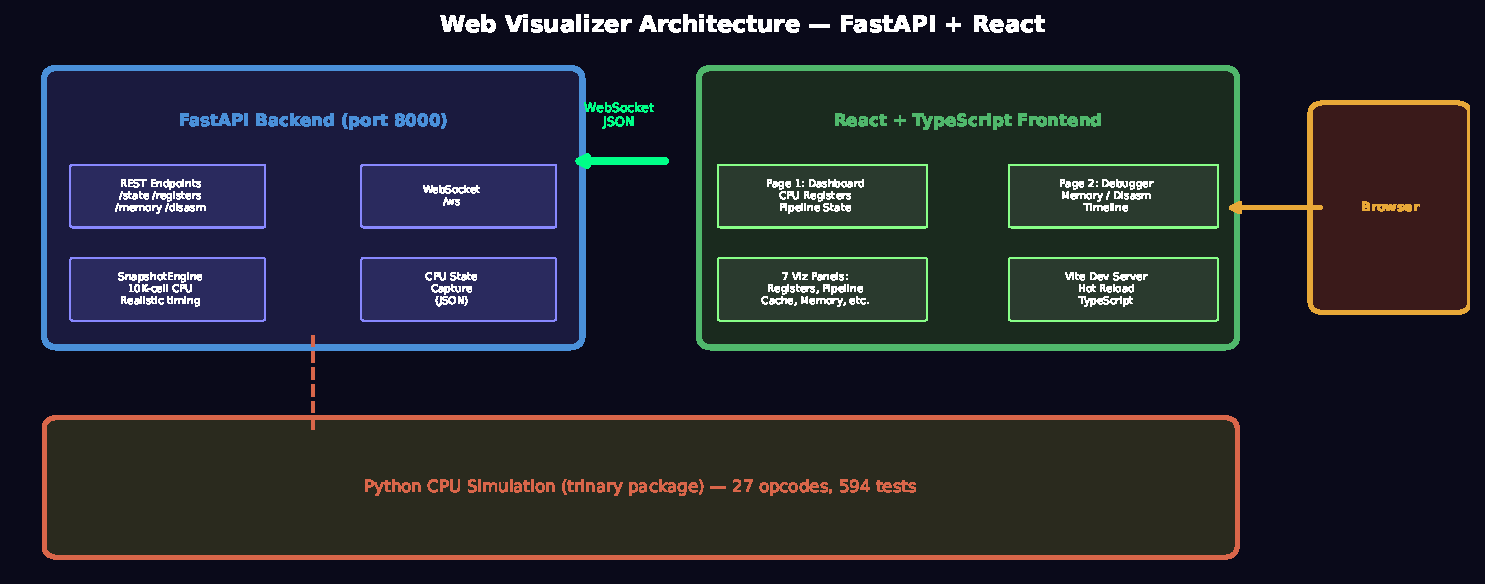
\includegraphics[width=0.68\textwidth]{webviz_architecture.pdf}
\caption{Web visualizer architecture — Python CPU simulation feeds the FastAPI backend through SnapshotEngine; React+TypeScript frontend connects via WebSocket for live state updates}
\label{fig:webvizarch}
\end{figure}

\section{System Architecture}

The web visualizer follows a strict client--server architecture:

\begin{verbatim}
+------------------------------------------------------------------+
|  Browser (React + TypeScript)                                    |
|  +----------+ +----------+ +--------------------+                 |
|  | Pipeline | |  Cache   | |  Branch, Timeline, |                 |
|  |  Visual  | | Heatmap  | |  Waveform, Bus     |                 |
|  +----------+ +----------+ +--------------------+                 |
|         |                  ^                                      |
|         v WebSocket        | WebSocket                            |
|  +----------------------------------------------------------+    |
|  |        FastAPI Server (port 8000)                         |    |
|  |  +--------------------------------------------------+    |    |
|  |  |       SnapshotEngine                              |    |    |
|  |  |  +------+ +-------+ +----------+                  |    |    |
|  |  |  | CPU  | |Machine| |  Memory  |                  |    |    |
|  |  |  +------+ +-------+ +----------+                  |    |    |
|  |  +--------------------------------------------------+    |    |
|  +----------------------------------------------------------+    |
+------------------------------------------------------------------+
\end{verbatim}

\section{Backend: FastAPI Web Server}

The backend (\texttt{backend/main.py}) is a FastAPI application running on
port 8000. It uses the \texttt{lifespan} async context manager pattern to
manage startup and shutdown: on startup, it creates an
\texttt{asyncio.create\_task} for a periodic broadcast loop; on shutdown,
the task is cancelled.

\subsection{SnapshotEngine}

The \texttt{SnapshotEngine} (\texttt{backend/snapshot\_engine.py}) is the
core bridge between the Trinary Python library and the web API. It
creates a \texttt{CPU} instance with \texttt{Memory(10000)} (supporting the
SDK framebuffer VRAM range at addresses 1000--5095) and
\texttt{realistic\_timing=True} for full hardware simulation.

The engine provides the following methods:
\begin{description}
    \item[\texttt{load\_program(source)}]: Calls \texttt{Machine.assemble()}
          to assemble the source, then \texttt{CPU.load\_program()} to
          load it into memory. Returns success status and metadata.
    \item[\texttt{step(count)}]: Steps the CPU by \texttt{count} cycles,
          capturing a full \texttt{SystemSnapshot} after each step.
    \item[\texttt{run\_to\_halt()}]: Steps the CPU until \texttt{cpu.halted}
          is true, capturing all intermediate snapshots.
    \item[\texttt{reset()}]: Resets CPU state and reloads the program.
    \item[\texttt{capture()}]: Reads the complete CPU state into a
          \texttt{SystemSnapshot} dataclass.
\end{description}

\subsection{SystemSnapshot Data Contract}

The \texttt{capture()} method produces a \texttt{SystemSnapshot} dataclass
containing:

\begin{itemize}
    \item \textbf{Core state}: cycle count, clock cycle, PC, SP, halted
          flag, registers (R0--R3 as ternary strings), condition flags,
          current instruction, instructions loaded count, wall-clock
          timestamp;
    \item \textbf{Pipeline state}: IF/ID/EX/MEM/WB stage contents,
          including instruction, opcode, bubble flag, and stall status;
    \item \textbf{Cache state}: hits, misses, hit rate, and line table
          (tag, valid, dirty) for both L1I and L1D;
    \item \textbf{Branch predictor state}: mode, predictions,
          mispredictions, accuracy, and the 2-bit counter table;
    \item \textbf{Bus state}: transfers, pending count, utilization,
          idle cycles;
    \item \textbf{DMA state}: active flag, queued transfers, completed
          transfers, progress;
    \item \textbf{Interrupt state}: pending interrupt count, in-ISR flag;
    \item \textbf{Profiler state}: cycles, instructions retired, CPI,
          IPC, total stalls, cache hit rate, branch accuracy.
\end{itemize}

\subsection{REST Endpoints}

\begin{table}[H]
\centering
\caption{FastAPI REST endpoint summary}
\label{tab:restendpoints}
\begin{tabular}{lll}
\toprule
Method & Path & Description \\
\midrule
GET  & \texttt{/api/status}  & CPU status summary \\
POST & \texttt{/api/load}    & Load assembly source \\
POST & \texttt{/api/step}    & Step N cycles \\
POST & \texttt{/api/run}     & Run to halt \\
POST & \texttt{/api/reset}   & Reset CPU \\
GET  & \texttt{/api/snapshot}& Get current snapshot \\
GET  & \texttt{/api/demos}   & List demo programs \\
\bottomrule
\end{tabular}
\end{table}

\subsection{WebSocket Protocol}

The primary communication channel is the WebSocket endpoint at
\texttt{/ws}. On connection, the server immediately sends the current
CPU snapshot, connection status, and the list of available demo programs.
The protocol defines the following message types:

\begin{description}
    \item[Client $\rightarrow$ Server]:
          \texttt{load} (with source code), \texttt{step} (with optional
          count), \texttt{run}, \texttt{reset}, \texttt{get\_default\_demo}.
    \item[Server $\rightarrow$ Client]:
          \texttt{snapshot} (full CPU state), \texttt{status} (connection
          status), \texttt{load\_result} (assembly result),
          \texttt{demos} (available programs).
\end{description}

A background broadcast loop runs at 20 FPS (50 ms intervals) while the
CPU is not halted, streaming snapshot updates to all connected WebSocket
clients for real-time visualization.

\subsection{WebSocket Message Format}

All WebSocket messages are JSON-encoded. Client-to-server commands follow
a uniform structure:

\begin{verbatim}
// Client → Server: command messages
{ "type": "load",    "source": "LOAD R0 10\n..." }
{ "type": "step",    "count": 5 }
{ "type": "run" }
{ "type": "reset" }
{ "type": "get_default_demo" }

// Server → Client: response messages
{ "type": "snapshot",     "data": { ... SystemSnapshot ... } }
{ "type": "status",       "status": "connected", "cpu": "running" }
{ "type": "load_result",  "success": true, "error": null }
{ "type": "demos",        "demos": ["Countdown", "Fibonacci", ...] }
\end{verbatim}

The \texttt{snapshot} message contains the full \texttt{SystemSnapshot}
dataclass serialised as JSON, including register values, pipeline state,
cache state, profiler metrics, and a 12-element demo program list.

\section{Frontend: React + TypeScript}

The frontend (\texttt{frontend/}) is a single-page application built with
React 18, Vite 5, TypeScript 5, and Tailwind CSS 3.

\subsection{Component Architecture}

The application consists of two pages:
\begin{description}
    \item[\texttt{LandingPage} (\texttt{/})]: An animated splash page with
          floating ternary digit particles, an animated datapath SVG,
          CRT scanline overlay, glitch text effects, and architecture
          badges. A ``Launch Simulator'' button navigates to the
          workspace.
    \item[\texttt{SimulatorPage} (\texttt{/simulator})]: The main
          two-panel workspace.
\end{description}

\subsection{SimulatorPage Layout}

The workspace is divided into three zones:

\paragraph{Header toolbar:} Logo, connection status indicator (animated
green/red pulsing dot), Step/Run/Reset buttons with hover glow effects,
and a real-time cycle/PC/instruction display.

\paragraph{Left panel (fixed 320px width):}
\begin{itemize}
    \item \textbf{Assembly Editor}: drop-down demo selector (17 curated
          demo programs), monospace textarea with syntax-coloured
          display, Load button, and result status bar.
    \item \textbf{Register View}: R0--R3 displayed as animated 4-digit
          trit displays with per-digit flip animation on value change.
          Digits are colour-coded (0 = gray, 1 = cyan, 2 = purple).
          PC (amber) and SP (magenta) values with condition flags shown
          as pill badges.
\end{itemize}

\paragraph{Centre panel (flexible width):} Seven tabbed visualization
panels:

\begin{enumerate}
    \item \textbf{Pipeline}: Five-stage pipeline diagram with
          colour-coded stage boxes (IF blue, ID green, EX amber, MEM red,
          WB purple), active stage glow animation, stall/bubble badges,
          and statistics counters.
    \item \textbf{Datapath}: Full SVG datapath diagram with animated
          pulse lines along active data paths. Paths are colour-coded by
          operation type (register reads purple, ALU orange, memory cyan,
          cache blue, DMA orange, branches pink).
    \item \textbf{Cache Heatmap}: 16 $\times$ 2 grid of cache lines for
          both L1I and L1D. Cells colour-coded green (valid), yellow
          (dirty), or dark (invalid) with per-cache hit/miss counters
          and hit rate.
    \item \textbf{Branch Predictor}: Four stat cards (mode, predictions,
          mispredictions, accuracy) with an animated accuracy progress
          bar and a 2-bit saturating counter state machine diagram.
    \item \textbf{Execution Timeline}: Scrollable table of instruction
          history with columns for sequence number, instruction text, PC,
          cycle, and register values. Register colour indicates non-zero
          (green) vs.\ zero (gray).
    \item \textbf{Waveform Viewer}: SVG-based digital signal display
          with named signal rows (clk, pc, sp, halted, cache\_hit,
          branch\_taken, int, dma, bus), proper clock rising/falling
          edges, horizontal scroll, zoom slider, and 40-cycle window.
    \item \textbf{Bus Visualizer}: Stat cards for transfers, pending
          count, utilization, and DMA activity, with an SVG bus topology
          diagram showing the central bus connected to CPU, DMA, VRAM,
          and ACCEL nodes.
\end{enumerate}

\subsection{WebSocket Hook}

The \texttt{useWebSocket} custom React hook manages the WebSocket
connection lifecycle:
\begin{itemize}
    \item Auto-connects on component mount to \texttt{ws://host/ws};
    \item Auto-reconnects with 2-second delay on disconnect;
    \item Dispatches incoming JSON messages by type to the appropriate
          React state setters;
    \item Provides command functions (\texttt{loadProgram()},
          \texttt{step()}, \texttt{run()}, \texttt{reset()}) that
          send the corresponding WebSocket messages;
    \item On connect, automatically requests the demo programs list.
\end{itemize}

\subsection{State Management}

All state is managed through React hooks (no Redux or context providers).
The \texttt{SimulatorPage} maintains:
\begin{itemize}
    \item \texttt{snapshot}: the most recent \texttt{SystemSnapshot} from
          the backend;
    \item \texttt{demos}: the list of available demo programs;
    \item \texttt{loadResult}: the result of the last assembly attempt;
    \item \texttt{executionHistory}: a rolling buffer of up to 100
          timeline entries for the execution timeline tab;
    \item \texttt{signalHistory}: 120-sample rolling buffer for waveform
          data, with synthetic signals derived from the snapshot.
\end{itemize}

\subsection{Visual Design}

The UI follows a dark cyberpunk aesthetic: background \texttt{\#0a0a1a},
cyber-cyan accents (\texttt{\#00ff88}), purple highlights
(\texttt{\#8888ff}), and magenta accents (\texttt{\#ff4488}). A CRT
scanline overlay with radial vignette is applied globally. Panel
components use glass-morphism styling with semi-transparent backgrounds
and backdrop blur. Custom Tailwind colour palette and animation classes
provide consistent styling across all visualizer components.

\section{Integration with the Trinary System}

The web visualizer instantiates the same \texttt{CPU} class used by all
other tools: the OS shell, PyQt6 UI, TAL compiler, and test suite. This
guarantees behavioural consistency across all interfaces.

\begin{table}[H]
\centering
\caption{Web visualizer component dependencies}
\label{tab:webdepts}
\begin{tabular}{ll}
\toprule
Component & Trinary Dependency \\
\midrule
SnapshotEngine & \texttt{trinary.cpu.CPU}, \texttt{trinary.machine.Machine}, \texttt{trinary.memory.Memory} \\
Hardware state & \texttt{trinary.hardware.*} (pipeline, cache, BP, bus, DMA, INTC) \\
Demo programs & \texttt{trinary.ui.demos} (shared with PyQt6 UI) \\
TAL support & Paste-able into editor (not directly imported) \\
\bottomrule
\end{tabular}
\end{table}

The \texttt{SnapshotEngine} is a strict read-only wrapper: it accesses
CPU state exclusively through public APIs and never mutates internal CPU
state directly. Every \texttt{step()} call produces a complete state
snapshot, making the visualisation cycle-accurate.

\section{Deployment}

\subsection{Backend}
\begin{verbatim}
pip install fastapi uvicorn websockets pydantic
cd backend && uvicorn main:app --host 0.0.0.0 --port 8000
\end{verbatim}

\subsection{Frontend}
\begin{verbatim}
cd frontend && npm install
npm run dev          # Development on port 5173
npm run build        # Production build
npm run preview      # Serve production build
\end{verbatim}

The Vite development server proxies \texttt{/api} and \texttt{/ws} to
\texttt{localhost:8000}, enabling seamless development without CORS
configuration.

\appendix

%====================================================================
\chapter{Test Suite Reference}
\label{app:tests}

The Trinary system is validated by 594 unit tests across 36 test files:

\begin{longtable}{llr}
\caption{Complete test suite organization}
\label{tab:testsuite} \\
\toprule
Test File & Focus & Tests \\
\midrule
\endfirsthead
\multicolumn{3}{c}{(\emph{continued})} \\
\toprule
Test File & Focus & Tests \\
\midrule
\endhead
\bottomrule
\endfoot
\texttt{test\_accelerator.py} & Accelerator tensor operations & 70 \\
\texttt{test\_activations.py} & Neural network activation functions & 14 \\
\texttt{test\_alu.py} & ALU operations (ADD through CMP) & 10 \\
\texttt{test\_arithmetic.py} & Decimal round-trip arithmetic & 12 \\
\texttt{test\_assembler.py} & Two-pass assembler, labels, comments & 5 \\
\texttt{test\_branch\_predictor.py} & Static and dynamic prediction & 7 \\
\texttt{test\_bus.py} & System bus arbitration & 7 \\
\texttt{test\_cache.py} & Direct-mapped L1 cache & 10 \\
\texttt{test\_conversion.py} & Ternary/decimal/binary conversion & 10 \\
\texttt{test\_cpu.py} & All 27 opcodes, flags, stacks, interrupts & 24 \\
\texttt{test\_cpu\_accelerator.py} & CPU + accelerator integration & 11 \\
\texttt{test\_cpu\_stress.py} & Nested calls, heavy loops, random sequences & 8 \\
\texttt{test\_datasets.py} & Neural network datasets & 10 \\
\texttt{test\_display.py} & Text display, keyboard, STOREM/LOADM & 20 \\
\texttt{test\_display\_framebuffer.py} & Framebuffer display & 20 \\
\texttt{test\_dma.py} & DMA transfers, concurrency & 7 \\
\texttt{test\_gpu.py} & GPU mode, warps, streams, native C, visualization & 71 \\
\texttt{test\_interrupts.py} & Interrupt controller (8-line) & 8 \\
\texttt{test\_losses.py} & Neural network loss functions & 10 \\
\texttt{test\_native\_backend.py} & Native C bridge (ctypes) & 11 \\
\texttt{test\_optimizers.py} & Neural network optimizers & 12 \\
\texttt{test\_os.py} & OS shell, kernel, terminal & 38 \\
\texttt{test\_packed\_trits.py} & Packed trit storage & 20 \\
\texttt{test\_perceptron.py} & Perceptron implementation & 16 \\
\texttt{test\_pipeline.py} & Clock, pipeline stages, hazards, timing & 19 \\
\texttt{test\_profiler.py} & Profiler metrics (CPI, IPC) & 9 \\
\texttt{test\_realistic\_cpu.py} & Full CPU with realistic timing & 9 \\
\texttt{test\_sdk.py} & Fantasy Console SDK (engine, runtime) & 50 \\
\texttt{test\_simd.py} & SIMD processor, vector lanes & 11 \\
\texttt{test\_tal.py} & TAL compiler & 12 \\
\texttt{test\_tensor\_core.py} & Tensor core matrix multiply & 12 \\
\texttt{test\_ternary\_nn.py} & Neural network (full pipeline) & 36 \\
\texttt{test\_trainer.py} & Neural network trainer & 20 \\
\texttt{test\_trit\_tensor.py} & Trit tensor operations & 10 \\
\texttt{test\_vector\_ops.py} & Vector operations & 12 \\
\texttt{test\_viz\_engine.py} & Visualization engine & 22 \\
\texttt{test\_vram.py} & VRAM controller timing & 7 \\
\midrule
\textbf{Total} & & \textbf{594} \\
\end{longtable}

The complete suite runs in approximately 0.4 seconds on modern hardware.

\begin{figure}[H]
\centering
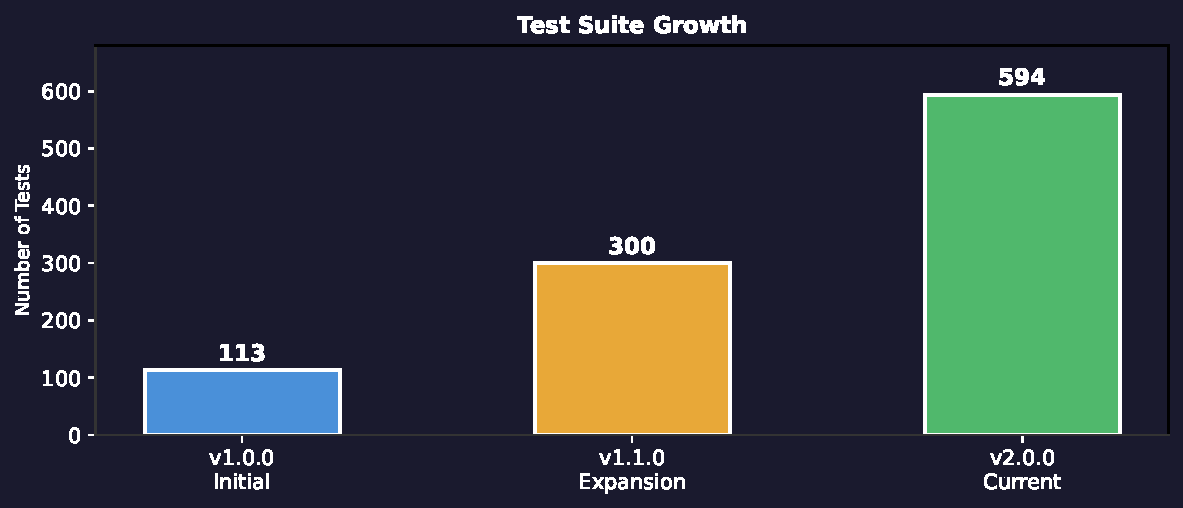
\includegraphics[width=0.72\textwidth]{test_growth.pdf}
\caption{Test suite growth from 113 initial tests through 300 in the expansion phase to 594 in the current version}
\label{fig:testgrowth}
\end{figure}

\begin{figure}[H]
\centering
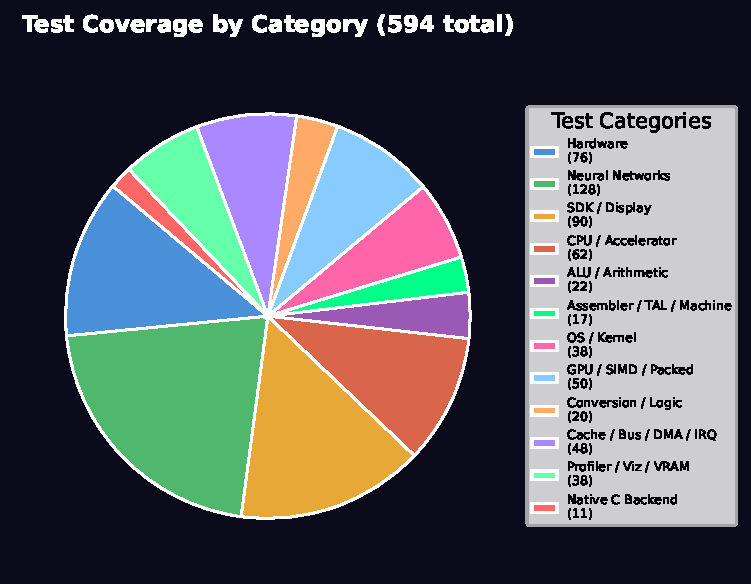
\includegraphics[width=0.68\textwidth]{test_coverage.pdf}
\caption{Test coverage by category (594 tests) — hardware, neural networks, SDK/display, CPU/accelerator, and supporting subsystems}
\label{fig:testcov}
\end{figure}

%====================================================================
\chapter{Performance Benchmarks}
\label{app:benchmarks}

\section{Digit Efficiency: Ternary vs.\ Binary}

\begin{figure}[H]
\centering
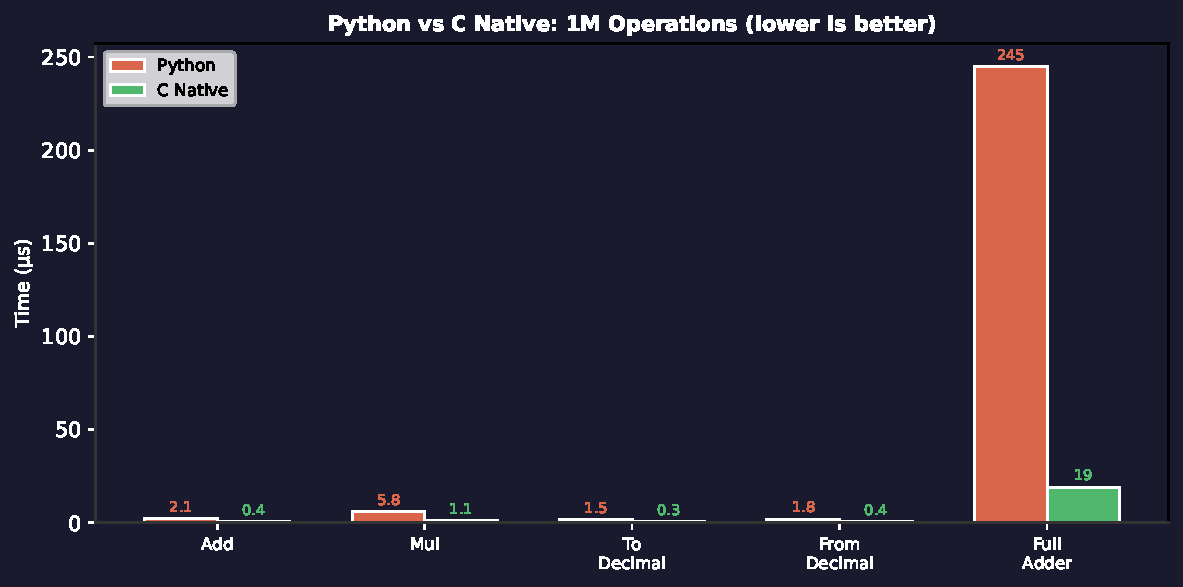
\includegraphics[width=0.62\textwidth]{benchmarks.pdf}
\caption{Benchmark comparison — native C backend speedup across four core ALU operations (5--13$\times$ improvement)}
\label{fig:benchmarks}
\end{figure}

\begin{table}[H]
\centering
\caption{Digit comparison across value ranges}
\label{app:digitcomp}
\begin{tabular}{crrr}
\toprule
Decimal Value & Binary Digits & Ternary Digits & Savings \\
\midrule
0 & 1 & 1 & 0\% \\
10 & 4 & 3 & 25\% \\
100 & 7 & 5 & 29\% \\
1,000 & 10 & 7 & 30\% \\
10,000 & 14 & 9 & 36\% \\
100,000 & 17 & 11 & 35\% \\
1,000,000 & 20 & 13 & 35\% \\
100,000,000 & 27 & 17 & 37\% \\
\bottomrule
\end{tabular}
\end{table}

\section{Execution Rate}

\begin{table}[H]
\centering
\caption{Execution throughput by configuration}
\label{app:execrate}
\begin{tabular}{lrr}
\toprule
Metric & Pure Python & With C Backend \\
\midrule
Simple instruction (LOAD, ADD) & $\sim$1M ops/sec & $\sim$5M ops/sec \\
Complex instruction (DIV) & $\sim$200K ops/sec & $\sim$800K ops/sec \\
Full demo program & $\sim$50K cycles/sec & $\sim$250K cycles/sec \\
594-test suite & $\sim$0.4s total & --- \\
\bottomrule
\end{tabular}
\end{table}

\section{Native C Backend Speedup}

\begin{table}[H]
\centering
\caption{Per-operation native C speedup (1M iterations)}
\label{app:nativeperf}
\begin{tabular}{lrrr}
\toprule
Operation & Python ($\mu$s) & C Native ($\mu$s) & Speedup \\
\midrule
Ternary add (10 trits) & 2.1 & 0.4 & 5.3$\times$ \\
Ternary mul (10 trits) & 5.8 & 1.1 & 5.3$\times$ \\
Ternary to decimal & 1.5 & 0.3 & 5.0$\times$ \\
Decimal to ternary & 1.8 & 0.4 & 4.5$\times$ \\
Full adder & 245 & 19 & 12.9$\times$ \\
\bottomrule
\end{tabular}
\end{table}

\section{Hardware Simulation Overhead}

\begin{table}[H]
\centering
\caption{Hardware microarchitecture overhead}
\label{app:hwperf}
\begin{tabular}{lr}
\toprule
Component & Measured Overhead \\
\midrule
Pipeline (5-stage) & $\sim$2$\times$ instruction count \\
Cache (direct-mapped L1) & $\sim$1--5\% miss rate \\
Branch predictor (2-bit) & $\sim$85--95\% accuracy \\
DMA (concurrent) & $\sim$10--30\% bus contention \\
Full realistic mode & $\sim$3--5$\times$ slower than fast mode \\
\bottomrule
\end{tabular}
\end{table}

\section{Memory Usage}

\begin{table}[H]
\centering
\caption{System memory footprint}
\label{app:memusage}
\begin{tabular}{lr}
\toprule
Component & Size \\
\midrule
Register file & 4 ternary strings \\
Memory (default config) & 512 cells \\
Memory (SDK config) & 10,000 cells \\
Stack region & $\sim$128 cells (addresses 128--255) \\
VRAM (text mode) & 56 cells (200--255) \\
VRAM (framebuffer) & 4,096 cells (1000--5095) \\
100-instruction program & $\sim$100 instruction strings \\
\bottomrule
\end{tabular}
\end{table}

\section{SDK / Fantasy Console Performance}

\begin{table}[H]
\centering
\caption{SDK game loop metrics}
\label{app:sdkperf}
\begin{tabular}{lr}
\toprule
Metric & Value \\
\midrule
Target FPS & 30 \\
Framebuffer size & 64 $\times$ 64 = 4,096 pixels \\
Sprite blit (8$\times$8) & $\sim$5$\mu$s \\
Tilemap render (32$\times$32) & $\sim$200$\mu$s \\
Particle update (50 particles) & $\sim$100$\mu$s \\
Full game loop (Pong) & $\sim$1ms per frame \\
\bottomrule
\end{tabular}
\end{table}

\section{Test Suite Growth}

\begin{table}[H]
\centering
\caption{Test suite evolution by version}
\label{app:testgrowth}
\begin{tabular}{lrr}
\toprule
Version & Tests & Run Time \\
\midrule
v1.0.0 (initial) & 113 & $\sim$0.06s \\
v1.1.0 (expansion) & 26 opcodes, display, interrupts & --- \\
v2.0.0 (current) & 594 & $\sim$0.4s \\
\bottomrule
\end{tabular}
\end{table}

%====================================================================
\chapter{Developer Reference}
\label{app:devguide}

\section{Adding a New Instruction}

\begin{enumerate}
    \item Add opcode to \texttt{OPCODE\_MAP} in \texttt{machine.py}. The opcode must
          be a unique 3-trit string.
    \item Add to \texttt{OPCODES} set and \texttt{CYCLES} dict in \texttt{cpu.py}.
    \item Implement execution logic in \texttt{cpu.execute\_instruction()} as a new
          branch in the opcode dispatch.
    \item Add encoding support in \texttt{machine.encode\_instruction()} if using a new
          format.
    \item Write tests in \texttt{tests/test\_cpu.py}.
    \item Update documentation and opcode count references.
\end{enumerate}

\section{Adding a New ALU Operation}

\begin{enumerate}
    \item Add to \texttt{VALID\_OPERATIONS} tuple in \texttt{alu.py}.
    \item Implement the operation logic in the \texttt{alu()} function.
    \item Connect in CPU: the CPU calls \texttt{alu("OP", a, b)} and writes the result.
    \item Write ALU unit tests.
\end{enumerate}

\section{Building and Running}

\begin{verbatim}
# Build native C backend
make -C src/trinary/native
bash build_native.sh

# Run all tests
python -m pytest tests/ -v

# Single test file
python -m pytest tests/test_cpu.py -v

# Keyword filter
python -m pytest tests/ -k "cmp" -v
\end{verbatim}

%====================================================================
% Bibliography
%====================================================================

\begin{thebibliography}{99}

\bibitem{knuth1997art}
D.~E.~Knuth, \emph{The Art of Computer Programming, Volume 2: Seminumerical
Algorithms}, 3rd~ed. Addison-Wesley, 1997.

\bibitem{brusentsov1965setun}
N.~P.~Brusentsov, ``The Setun computer,'' \emph{Proceedings of the IFIP Congress},
vol.~2, pp.~411--412, 1965.

\bibitem{hurts1989comparison}
S.~L.~Hurst, ``Multiple-valued logic --- its status and its future,''
\emph{IEEE Transactions on Computers}, vol.~33, no.~12, pp.~1160--1179, 1984.

\bibitem{smith1997mvl}
K.~C.~Smith, ``Multiple-valued logic: a tutorial and appreciation,''
\emph{IEEE Computer}, vol.~21, no.~4, pp.~17--27, 1988.

\bibitem{epstein1985mvl}
G.~Epstein, ``Multiple-valued logic design: an introduction,''
\emph{Proceedings of the IEEE}, vol.~73, no.~2, pp.~322--334, 1985.

\bibitem{ternarycpu}
Trinary Project Repository, \url{https://github.com/anomalyco/ternarycpu}.

\bibitem{mcculloch1943logical}
W.~S.~McCulloch and W.~Pitts, ``A logical calculus of the ideas immanent in nervous
activity,'' \emph{Bulletin of Mathematical Biophysics}, vol.~5, pp.~115--133, 1943.

\bibitem{rosenblatt1958perceptron}
F.~Rosenblatt, ``The perceptron: a probabilistic model for information storage and
organization in the brain,'' \emph{Psychological Review}, vol.~65, no.~6,
pp.~386--408, 1958.

\bibitem{rumelhart1986learning}
D.~E.~Rumelhart, G.~E.~Hinton, and R.~J.~Williams, ``Learning representations by
back-propagating errors,'' \emph{Nature}, vol.~323, pp.~533--536, 1986.

\bibitem{lapedes1994neural}
A.~Lapedes and R.~Farber, ``How neural networks work,'' in \emph{Neural Information
Processing Systems}, pp.~442--456, 1987.

\bibitem{lecun2015deep}
Y.~LeCun, Y.~Bengio, and G.~Hinton, ``Deep learning,'' \emph{Nature}, vol.~521,
pp.~436--444, 2015.

\end{thebibliography}

\end{document}
